\documentclass[a4paper,12pt,twoside]{memoir}

% Castellano
\usepackage[spanish,es-tabla]{babel}
\selectlanguage{spanish}
\usepackage[utf8]{inputenc}
\usepackage[T1]{fontenc}
\usepackage{lmodern} % Scalable font
\usepackage{microtype}
\usepackage{placeins}
\usepackage{enumitem}
\usepackage{float}
\usepackage{longtable}
\usepackage[justification=centering]{caption}



\RequirePackage{booktabs}
\RequirePackage[table]{xcolor}
\RequirePackage{xtab}
\RequirePackage{multirow}

% Links
\PassOptionsToPackage{hyphens}{url}\usepackage[colorlinks]{hyperref}
\hypersetup{
	allcolors = {red}
}

% Ecuaciones
\usepackage{amsmath}

% Rutas de fichero / paquete
\newcommand{\ruta}[1]{{\sffamily #1}}

% Párrafos
\nonzeroparskip

% Huérfanas y viudas
\widowpenalty100000
\clubpenalty100000

\let\tmp\oddsidemargin
\let\oddsidemargin\evensidemargin
\let\evensidemargin\tmp
\reversemarginpar

% Imágenes

% Comando para insertar una imagen en un lugar concreto.
% Los parámetros son:
% 1 --> Ruta absoluta/relativa de la figura
% 2 --> Texto a pie de figura
% 3 --> Tamaño en tanto por uno relativo al ancho de página
\usepackage{graphicx}

\newcommand{\imagen}[3]{
	\begin{figure}[!h]
		\centering
		\includegraphics[width=#3\textwidth]{#1}
		\caption{#2}\label{fig:#1}
	\end{figure}
	\FloatBarrier
}







\graphicspath{ {./img/} }

% Capítulos
\chapterstyle{bianchi}
\newcommand{\capitulo}[2]{
	\setcounter{chapter}{#1}
	\setcounter{section}{0}
	\setcounter{figure}{0}
	\setcounter{table}{0}
	\chapter*{#2}
	\addcontentsline{toc}{chapter}{#2}
	\markboth{#2}{#2}
}

% Apéndices
\renewcommand{\appendixname}{Apéndice}
\renewcommand*\cftappendixname{\appendixname}

\newcommand{\apendice}[1]{
	%\renewcommand{\thechapter}{A}
	\chapter{#1}
}

\renewcommand*\cftappendixname{\appendixname\ }

% Formato de portada

\makeatletter
\usepackage{xcolor}
\newcommand{\tutor}[1]{\def\@tutor{#1}}
\newcommand{\tutorb}[1]{\def\@tutorb{#1}}

\newcommand{\course}[1]{\def\@course{#1}}
\definecolor{cpardoBox}{HTML}{E6E6FF}
\def\maketitle{
  \null
  \thispagestyle{empty}
  % Cabecera ----------------
\begin{center}
  \noindent
\includegraphics[width=\textwidth]{cabeceraSalud}\vspace{1.5cm}%
\end{center}
  
  % Título proyecto y escudo salud ----------------
  \begin{center}
    \begin{minipage}[c][1.5cm][c]{.20\textwidth}
        
\includegraphics[width=\textwidth]{escudoSalud.pdf}
    \end{minipage}
  \end{center}
  
  \begin{center}
    \colorbox{cpardoBox}{%
        \begin{minipage}{.8\textwidth}
          \vspace{.5cm}\Large
          \begin{center}
          \textbf{TFG del Grado en Ingeniería de la Salud}\vspace{.6cm}\\
          \textbf{\LARGE\@title{}}
          \end{center}
          \vspace{.2cm}
        \end{minipage}
    }%
  \end{center}
  
    % Datos de alumno, curso y tutores ------------------
  \begin{center}%
  {%
    \noindent\LARGE
    Presentado por \@author{}\\ 
    en Universidad de Burgos\\
    \vspace{0.5cm}
    \noindent\Large
    \@date{}\\
    \vspace{0.5cm}
    Tutor: \@tutor{}\\ % comenta el que no corresponda
    %Tutores: \@tutor{} -- \@tutorb{}\\
  }%
  \end{center}%
  \null
  \cleardoublepage
  }
\makeatother

\newcommand{\nombre}{Marina Martín Marijuán}
\newcommand{\nombreTutor}{Telmo Miguel Medina} 
%\newcommand{\nombreTutorb}{Tutor 2} 
\newcommand{\dni}{13172541G} 

% Datos de portada
\title{Aplicación web para la predicción de trastornos del sueño con apoyo del dispositivo O2Ring}
\author{\nombre}
\tutor{\nombreTutor}
%\tutorb{\nombreTutorb}
\date{\today}


\begin{document}

\maketitle


\newpage\null\thispagestyle{empty}\newpage

%%%%%%%%%%%%%%%%%%%%%%%%%%%%%%%%%%%%%%%%%%%%%%%%%%%%%%%%%%%%%%%%%%%%%%%%%%%%%%%%%%%%%%%%
\thispagestyle{empty}


\noindent
\includegraphics[width=\textwidth]{cabeceraSalud}\vspace{1cm}

\noindent D. \nombreTutor, profesor del departamento de departamento, área de área.

\noindent Expone:

\noindent Que el alumno D. \nombre, con DNI \dni, ha realizado el Trabajo final de Grado en Ingeniería de la Salud titulado título del trabajo. 

\noindent Y que dicho trabajo ha sido realizado por el alumno bajo la dirección del que suscribe, en virtud de lo cual se autoriza su presentación y defensa.

\begin{center} %\large
En Burgos, {\large \today}
\end{center}

\vfill\vfill\vfill

% Author and supervisor
\begin{minipage}{0.45\textwidth}
\begin{flushleft} %\large
Vº. Bº. del Tutor:\\[2cm]
D. \nombreTutor
\end{flushleft}
\end{minipage}
\hfill
\begin{minipage}{0.45\textwidth}
\begin{flushleft} %\large
%Vº. Bº. del Tutor:\\[2cm]
%D. \nombreTutorb
\end{flushleft}
\end{minipage}
\hfill

\vfill

% para casos con solo un tutor comentar lo anterior
% y descomentar lo siguiente
%Vº. Bº. del Tutor:\\[2cm]
%D. nombre tutor


\newpage\null\thispagestyle{empty}\newpage




\frontmatter

% Abstract en castellano
\renewcommand*\abstractname{Resumen}
\begin{abstract}
La calidad del sueño ha cobrado una gran relevancia en los últimos años debido a su impacto directo en la salud física y mental. Trastornos como el insomnio o la apnea del sueño afectan significativamente la calidad de vida y su detección precoz continúa siendo un desafío, especialmente fuera del entorno clínico.

Este Trabajo de Fin de Grado presenta el desarrollo de un sistema de predicción basado en técnicas de aprendizaje automático, capaz de estimar la probabilidad de pertenencia a una de tres clases: insomnio, apnea del sueño o ausencia de trastorno. Para ello, se ha empleado un conjunto de datos abierto con información clínica, demográfica y de estilo de vida, sobre el cual se ha aplicado un proceso completo de análisis exploratorio, preprocesamiento, balanceo con SMOTE y calibración probabilística.

El modelo seleccionado, un Random Forest calibrado, ha sido integrado en una aplicación web desarrollada con Streamlit, que permite al usuario introducir sus datos, obtener una predicción multiclase en tiempo real y consultar una explicación visual de los factores que han influido en el resultado mediante gráficos SHAP. Además, la herramienta genera un informe en PDF personalizado y permite el acceso desde dispositivos móviles mediante código QR.

El sistema se plantea como una herramienta accesible, interpretable y de bajo coste computacional, útil como cribado inicial en contextos clínicos, educativos o de salud pública.


\end{abstract}

\renewcommand*\abstractname{Descriptores}
\begin{abstract}
Trastornos del sueño, insomnio, apnea del sueño, aprendizaje automático, modelo predictivo, aplicación web \ldots
\end{abstract}

\clearpage

% Abstract en inglés
\renewcommand*\abstractname{Abstract}
\begin{abstract}
Sleep quality has gained increasing relevance in recent years due to its direct impact on physical and mental health. Disorders such as insomnia or sleep apnea significantly reduce quality of life, and their early detection remains a challenge, especially outside clinical environments.

This Final Degree Project presents the development of a prediction system based on machine learning techniques, capable of estimating the likelihood of belonging to one of three classes: insomnia, sleep apnea, or no disorder. An open dataset containing clinical, demographic, and lifestyle information was used, and a complete process of exploratory analysis, data preprocessing, class balancing using SMOTE, and probabilistic calibration was applied.

The final model, a calibrated Random Forest, was integrated into an interactive web application developed with Streamlit. This platform allows users to input personal data, obtain a real-time multiclass prediction, and access a visual explanation of the factors influencing the result using SHAP plots. Additionally, the tool generates a personalized PDF report and supports access from mobile devices via QR code.

The system is proposed as an accessible, interpretable, and low-cost screening tool, potentially useful in clinical, educational, or public health contexts.

\end{abstract}

\renewcommand*\abstractname{Keywords}
\begin{abstract}
Sleep disorders, insomnia, sleep apnea, machine learning, predictive model, web application.
\end{abstract}

\clearpage

% Indices
\tableofcontents

\clearpage

\listoffigures

\clearpage

\listoftables
\clearpage

\chapter{Lista de abreviaturas}

\begin{longtable}{ll}
\textbf{Abreviatura} & \textbf{Significado} \\
\hline
NREM  & No Rapid Eye Movement \\
REM   & Rapid Eye Movement \\
AASM  & American Academy of Sleep Medicine \\
AOS   & Apnea Obstructiva del Sueño \\
ACS   & Apnea Central del Sueño \\
CPAP  & Continuous Positive Airway Pressure \\
SPI   & Síndrome de Piernas Inquietas \\
IMC   & Índice de Masa Corporal \\
OMS   & Organización Mundial de la Salud \\
FC    & Frecuencia Cardíaca \\
SpO\textsubscript{2} & Saturación de Oxígeno en Sangre \\
PPG   & Fotopletismografía \\
PSG   & Polisomnografía \\
EEG   & Electroencefalograma \\
EOG   & Electrooculograma \\
EMG   & Electromiograma \\
PR    & Poligrafía Respiratoria \\
HRV   & Heart Rate Variability \\
ODI   & Oxygen Desaturation Index \\
PSQI  & Pittsburgh Sleep Quality Index \\
ISI   & Insomnia Severity Index \\
ESS   & Epworth Sleepiness Scale \\
MSLT  & Multiple Sleep Latency Test \\
SSS   & Stanford Sleepiness Scale \\
ML    & Machine Learning \\
MLP   & Multilayer Perceptron \\
\end{longtable}



\mainmatter
\capitulo{1}{Introducción}

El sueño cobra un papel fundamental en la salud humana, influyendo directamente en las funciones fisiológicas, cognitivas y emocionales. La existencia de trastornos del sueño, como el insomnio o la apnea obstructiva del sueño, se ha asociado con un mayor riesgo de desarrollar enfermedades cardiovasculares, metabólicas y mentales, así como con una disminución significativa en la calidad de vida de quienes los padecen.

Se estima que hasta un 30\% de la población mundial presenta algún tipo de alteración en el sueño. Aunque no siempre se consideran enfermedades graves, estos trastornos constituyen un problema de salud pública debido a su alta prevalencia, su impacto funcional y las comorbilidades que pueden desencadenar. Además, conllevan importantes costes económicos derivados de las bajas laborales, la disminución del rendimiento y el aumento del riesgo de accidentes de tráfico o laborales.


Actualmente, el diagnóstico de estos trastornos requiere herramientas clínicas especializadas y costosas, siendo la polisomnografía el estándar de referencia para la detección de alteraciones respiratorias o neurológicas durante el sueño. En otros casos, el diagnóstico se basa en cuestionarios subjetivos, cuya fiabilidad depende en gran medida de la percepción del paciente. En este contexto, los avances en aprendizaje automático han abierto nuevas oportunidades para el cribado y la detección temprana de alteraciones del sueño mediante el uso de variables fácilmente recopilables como la edad, la ocupación, los hábitos de sueño o la presión arterial.


Este Trabajo de Fin de Grado plantea el desarrollo de un sistema predictivo basado en aprendizaje automático, capaz de estimar la probabilidad de que un individuo presente un trastorno del sueño a partir de variables clínicas y de estilo de vida. Para ello, se ha utilizado un conjunto de datos público, se han evaluado distintos modelos de clasificación y se ha implementado una aplicación interactiva que permite introducir información del usuario y obtener una predicción explicada mediante técnicas de interpretabilidad.

El sistema propuesto pretende servir como herramienta de cribado accesible y explicable, aportando valor tanto a profesionales sanitarios como a usuarios particulares, especialmente en contextos de atención primaria o educación para la salud. Gracias a su diseño accesible, su carácter interpretable y su automatización, puede facilitar una primera valoración objetiva sin necesidad de equipamiento médico especializado.

Este documento recoge todas las fases del proyecto: desde el análisis de datos y la selección del modelo hasta la implementación de la aplicación web. Finalmente, se analizan los resultados obtenidos, las limitaciones detectadas y las posibles líneas de mejora para futuros desarrollos.
\capitulo{2}{Objetivos}

La comprensión de los trastornos del sueño y su diagnóstico precoz constituyen un desafío relevante tanto para la investigación clínica como para la ingeniería aplicada a la salud. La integración de modelos de aprendizaje automático con herramientas digitales interactivas representa una oportunidad para facilitar la detección preliminar de patologías como el insomnio o la apnea del sueño mediante un sistema digital interpretable, accesible y reproducible.

Este trabajo surge con el propósito de combinar el análisis de datos con el desarrollo de una herramienta funcional que pueda ser utilizada por profesionales y usuarios como apoyo en la valoración inicial de problemas relacionados con el sueño.



\section{Objetivo principal}

Desarrollar un modelo de clasificación multiclase capaz de predecir la presencia de trastornos del sueño, concretamente insomnio, apnea del sueño o ausencia de patología; a partir de variables clínicas, demográficas y de estilo de vida, e integrarlo en una aplicación web interactiva orientada a profesionales y usuarios no técnicos, que facilite su uso e interpretación clínica inicial.

\section{Objetivos específicos}
\begin{enumerate}

\item  \textbf{Realizar un análisis estadístico del conjunto de datos clínicos y de estilo de vida}, con el fin de identificar posibles relaciones entre las variables clínicas, sociales y conductuales del conjunto de datos, y su influencia en los trastornos del sueño. Esta fase abarca tanto el análisis exploratorio como las etapas de limpieza, codificación, escalado y preparación del dataset para su posterior uso en modelos de aprendizaje automático.


\item \textbf{Diseñar y entrenar modelos de aprendizaje automático capaces de clasificar a los individuos} según su probabilidad de padecer insomnio, apnea del sueño o no presentar ningún trastorno, empleando como base las variables clínicas, sociales y conductuales analizadas previamente. Para ello, se evaluarán distintos algoritmos de clasificación, entre los que destacan Random Forest y redes neuronales multicapa (MLP).

\item \textbf{Optimizar, validar y comparar los modelos entrenados,} aplicando validación cruzada y evaluando su rendimiento mediante métricas como precisión, recall, F1-score y matriz de confusión. Se seleccionará el modelo con mejor rendimiento general y mayor capacidad de generalización; y se incorporarán técnicas de interpretabilidad como SHAP para analizar la importancia de las variables predictoras.

\item\textbf{Desarrollar una aplicación web interactiva mediante Streamlit} que permita introducir datos manualmente, realizar la predicción e interpretar los resultados de forma visual e intuitiva, facilitando así su uso por parte de usuarios sin conocimientos técnicos.

\item\textbf{Desplegar y documentar la herramienta}, incluyendo su publicación en la nube y la generación de un código QR que facilite el acceso desde dispositivos móviles, así como su demostración durante la exposición del trabajo.
\end{enumerate}


\section{Objetivos personales}

\begin{enumerate}
    \item Explorar el potencial del aprendizaje automático como herramienta de apoyo al diagnóstico temprano de enfermedades, contribuyendo al desarrollo de soluciones accesibles y escalables para fases iniciales de cribado en salud.
    \item Adquirir experiencia en el desarrollo de aplicaciones interactivas mediante el uso de tecnologías como Streamlit, GitHub o LaTeX, integrando competencias en programación, visualización de resultados y documentación técnica.
    \item Aplicar una perspectiva ingenieril a un problema clínico real, desarrollando una herramienta funcional que pueda escalarse o integrarse en sistemas clínicos más complejos en un futuro.
    \item Fomentar la autonomía y la capacidad de gestión de proyectos, planificando y ejecutando todas las fases de un sistema predictivo completo: desde el análisis de datos hasta su implementación y presentación final.
\end{enumerate}
\capitulo{3}{Conceptos teóricos}


\section{ Importancia de la calidad del sueño}

El sueño es un proceso biológico fundamental para la regulación de múltiples funciones fisiológicas, cognitivas y metabólicas. Su importancia radica en su papel en la homeostasis del organismo, la consolidación de la memoria, la regulación del estado anímico y la prevención de enfermedades crónicas. Estudios epidemiológicos han demostrado que una deficiencia en la calidad del sueño está asociada con un mayor riesgo de enfermedades cardiovasculares, metabólicas y psiquiátricas, así como con una reducción en el rendimiento cognitivo y una mayor incidencia de accidentes laborales y de tráfico  \cite{interactions}.

Desde el punto de vista fisiológico, el sueño se estructura en ciclos de aproximadamente 90 a 120 minutos que se repiten durante la noche, alternando entre dos grandes fases: sueño NREM (no REM) y sueño REM (movimientos oculares rápidos). El \textbf{sueño NREM} comprende tres estadios (N1, N2 y N3) según la clasificación actual de la AASM\footnote{Según la Academia Estadounidense de Medicina del Sueño: \url{https://aasm.org/}.}, que van desde el sueño ligero hasta el sueño profundo, asociado a la recuperación física y a la secreción de hormonas como la del crecimiento. Por su parte, el \textbf{sueño REM} se caracteriza por una intensa actividad cerebral, sueños vívidos y consolidación de la memoria emocional. La correcta alternancia entre estas fases es clave para un descanso reparador, y su alteración se ha relacionado con diversas patologías físicas y mentales \cite{sleepfoundation2023}.


\subsection{Impacto en la Funcionalidad Cognitiva}


El sueño profundo y, especialmente, la fase REM, desempeñan un papel esencial en la consolidación de la memoria y en procesos clave de aprendizaje. Según estudios en neurociencia, la privación del sueño disminuye la plasticidad neuronal y afecta negativamente a la consolidación de la memoria declarativa y procedimental \cite{funcionCognitiva}. Stickgold y Walker señalaron que la calidad del sueño influye directamente en la capacidad de procesamiento de información, la toma de decisiones y la regulación emocional \cite{calidadSueño}. En este sentido, Killgore observó que la privación parcial del sueño puede reducir la velocidad de reacción y aumentar la tasa de errores en tareas complejas \cite{efectosSueño}.


\subsection{Relación con Enfermedades Crónicas}

Numerosos estudios han establecido una fuerte correlación entre la deficiencia del sueño y la incidencia de enfermedades metabólicas y cardiovasculares. La restricción crónica del sueño se ha vinculado a una alteración en la regulación de la glucosa y a una disminución de la sensibilidad a la insulina, factores de riesgo clave para el desarrollo de diabetes tipo 2, como destacan Reutrakul y Van Cauter \cite{relacionEnfermedadesCronicas}. Asimismo, la falta de sueño se asocia con un aumento de la actividad simpática y niveles elevados de cortisol, lo que favorece el desarrollo de hipertensión y eventos cardiovasculares adversos. Un metaanálisis de Peppard et al. concluyó que los individuos con apnea obstructiva del sueño presentan un riesgo significativamente mayor de padecer hipertensión arterial \cite{hipertensionSueño}.



\subsection{Salud Mental y Bienestar Emocional}

El sueño y la salud mental tienen una relación bidireccional, es decir, se influyen mutuamente: la falta de sueño puede contribuir al desarrollo de trastornos psiquiátricos como la depresión y la ansiedad, mientras que estos mismos trastornos pueden alterar la calidad y estructura del sueño \cite{baglioni2016sleep}. Durante la fase REM, el cerebro procesa emociones y refuerza la resiliencia psicológica, lo cual justifica su asociación con alteraciones en la regulación emocional y un incremento en la irritabilidad y la impulsividad \cite{walker2009overnight}. Estudios clínicos han encontrado que la disrupción del sueño puede exacerbar síntomas en personas con trastornos del estado de ánimo, afectando la calidad de vida de los pacientes y aumentando el riesgo de episodios depresivos severos.

\subsection{Rendimiento Diario y Seguridad}

El impacto del sueño insuficiente en el desempeño de actividades cotidianas es significativo. La privación del sueño afecta la capacidad de concentración, la memoria operativa y el tiempo de reacción, lo que puede comprometer la seguridad en entornos laborales y de tráfico \cite{williamson2000moderate}. Dawson y Reid demostraron que permanecer despierto durante más de 17 horas genera un deterioro cognitivo comparable al de una intoxicación por alcohol con una concentración sanguínea de 0.05\%. La fatiga por falta de sueño es responsable de un alto porcentaje de accidentes laborales e incidentes de tráfico, representando un problema de salud pública \cite{dawson1997fatigue}.

\subsection{Relación con Trastornos del Sueño}

La calidad del sueño también está determinada por la presencia de trastornos específicos, como el insomnio, la apnea obstructiva del sueño y el síndrome de piernas inquietas. Peppard et al. identificaron una relación entre la apnea del sueño y un mayor riesgo de hipertensión \cite{peppard2000prospective}. El insomnio afecta a un porcentaje considerable de la población adulta, con prevalencias que oscilan entre el 10\% y el 30\%, dependiendo del criterio diagnóstico utilizado. Asimismo, el síndrome de piernas inquietas afecta entre el 2.5\% y el 15\% de la población general, impactando negativamente la continuidad y profundidad del sueño \cite{baglioni2016sleep}.


En conclusión, la calidad del sueño es un determinante crucial de la salud física y mental. La investigación en este campo es esencial para desarrollar estrategias preventivas y tecnologías innovadoras que permitan mejorar la higiene del sueño y mitigar los efectos adversos asociados a su deterioro. La integración de herramientas de evaluación del sueño basadas en modelos predictivos puede contribuir significativamente a la detección temprana y al tratamiento personalizado de trastornos del sueño, optimizando así la salud pública y la calidad de vida de la población.



\section{Trastornos del Sueño}


Los trastornos del sueño comprenden un conjunto de alteraciones que afectan la cantidad, calidad o estructura del sueño, y pueden tener un impacto significativo en el bienestar físico, mental y emocional de quienes los padecen. Estas alteraciones incluyen desde dificultades para iniciar o mantener el sueño hasta episodios respiratorios anómalos o conductas inusuales durante el descanso. En esta sección se describen los principales trastornos del sueño desde una perspectiva clínica, poniendo especial énfasis en aquellos con mayor prevalencia o relevancia para el desarrollo del sistema predictivo propuesto en este trabajo.

\subsection{Apnea del Sueño}
La apnea del sueño se caracteriza por episodios repetidos de obstrucción parcial o completa de la vía aérea superior durante el sueño, lo que provoca una disminución o cese del flujo respiratorio. Estos eventos suelen ir acompañados de desaturaciones de oxígeno y microdespertares que fragmentan el sueño, afectando así a la calidad de vida. 

El índice de apnea-hipopnea (AHI) es uno de los principales criterios diagnósticos, clasificando la apnea en leve (5–15 eventos/hora), moderada (15–30) o grave (más de 30 eventos/hora).

Existen varios tipos de apnea: 
\begin{itemize}
    \item \textbf{Apnea Obstructiva del Sueño (AOS)}: es el tipo más común de apnea y se caracteriza por una \textbf{reducción del flujo respiratorio superior al 90\% durante al menos 10 segundos}, en presencia de esfuerzo respiratorio. Esta obstrucción se debe a una relajación excesiva de los músculos de la garganta, lo que impide el paso adecuado del aire hacia los pulmones. Como consecuencia, se reduce la saturación de oxígeno en sangre y, ante esta situación, el cerebro desencadena breves microdespertares para reactivar la respiración, lo que fragmenta el sueño y deteriora su calidad.

Por otro lado, se habla de \textbf{hipoapnea} en el caso de que la reducción de la señal se encuentre entre el 30 y 90\%, con duración igual o menor a 10 segundos \textbf{y una disminución de la saturación mayor o igual al 3\%.}
\footnote{Imagen extraída de la memoria de prácticas realizada en la empresa Oxigen Salud.}.

\begin{figure}[H]
    \centering
    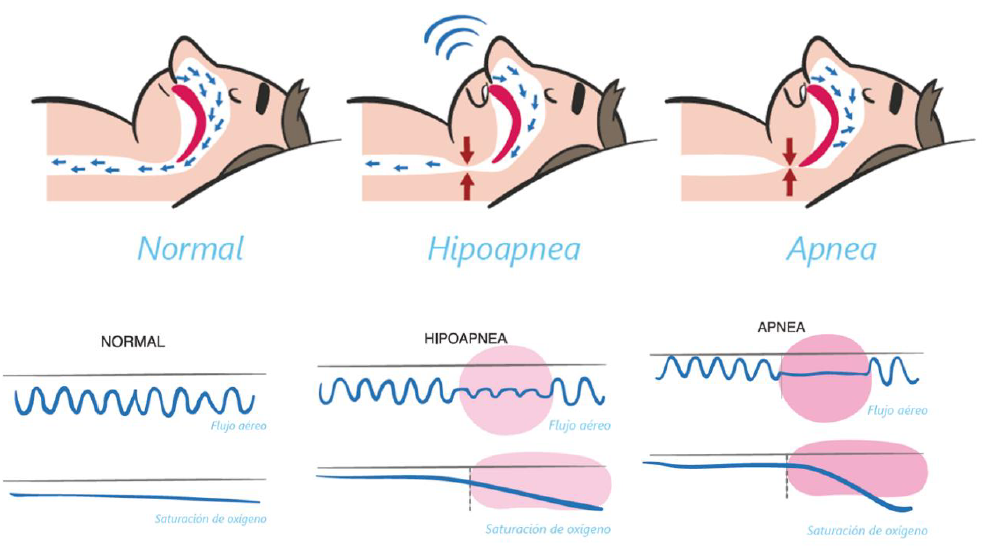
\includegraphics[width=0.75\linewidth]{img/AOS.png}
    \caption[Esquema comparativo de respiración normal, hipoapnea y apnea del sueño, junto con los respectivos patrones de flujo aéreo y saturación de oxígeno.]{Esquema comparativo de respiración normal, hipoapnea y apnea del sueño, junto con los respectivos patrones de flujo aéreo y saturación de oxígeno. Imagen adaptada de Oxigen Salud \cite{oxigensalud2025}.}
    \label{fig:AOS}
\end{figure}


\item  \textbf{Apnea Central del Sueño (ACS):} este tipo de apnea se produce por una \textbf{disfunción en el control de la respiración}, en la que el cerebro deja temporalmente de enviar señales a los músculos responsables de la respiración. A diferencia de la AOS, no existe una obstrucción física de las vías respiratorias, sino una falta de esfuerzo ventilatorio \footnote{El esfuerzo ventilatorio es la actividad muscular necesaria para permitir la entrada de aire a los pulmones.}

\item \textbf{Apnea Mixta:} combina características de la apnea central y la obstructiva. Habitualmente, un episodio comienza sin esfuerzo respiratorio (como en la apnea central) y continúa con una obstrucción de la vía aérea (como en la apnea obstructiva). Es frecuente en pacientes con formas graves de trastornos respiratorios del sueño.

\end{itemize}
El tratamiento se basa, en la mayoría de los casos, en el uso de presión positiva continua en las vías respiratorias (CPAP), que mantiene la vía aérea abierta durante el sueño y reduce los eventos de apnea. En casos leves pueden emplearse dispositivos de avance mandibular, mientras que en casos seleccionados se recurre a intervenciones quirúrgicas. Además, las modificaciones en el estilo de vida (como la pérdida de peso, evitar alcohol y sedantes y adoptar una postura adecuada al dormir) también son clave para una mejoría \cite{mayoclinic_apnea}.


\subsection{Insomnio}
El insomnio es uno de los trastornos del sueño más comunes y se manifiesta como una dificultad persistente para iniciar o mantener el sueño, o bien como un despertar temprano con incapacidad para volver a dormir. Estas alteraciones provocan un deterioro significativo en el funcionamiento diurno del individuo. La prevalencia de este trastorno oscila entre el 10\% y el 30\% de la población general, y puede llegar hasta el 50\% en grupos específicos como personas mayores o con comorbilidades psiquiátricas \cite{morin2012chronic}.

Se distinguen dos formas principales: el \textbf{insomnio agudo}, que dura días o semanas y suele estar relacionado con factores estresantes temporales; y el \textbf{insomnio crónico}, que persiste al menos tres veces por semana durante un mínimo de tres meses. 

Entre los factores de riesgo se incluyen el estrés crónico, trastornos de ansiedad y depresión, enfermedades médicas (como dolor crónico, enfermedad pulmonar obstructiva crónica o insuficiencia cardíaca), así como hábitos de sueño irregulares, uso de estimulantes y envejecimiento \cite{ninds_narcolepsy}.

Para su diagnóstico, se utilizan cuestionarios estandarizados como el \textbf{Índice de Severidad del Insomnio (ISI)}, registros de sueño y diarios del sueño. En casos concretos, pueden utilizarse técnicas adicionales como la \textbf{actigrafía} o la \textbf{polisomnografía}, especialmente si se sospecha la presencia de otros trastornos del sueño asociados, como la apnea \cite{ISI}.


\subsection{Narcolepsia}
La narcolepsia es un trastorno neurológico crónico que afecta la regulación del sueño-vigilia. Se caracteriza por una \textbf{somnolencia diurna excesiva} y episodios involuntarios de sueño. Otros síntomas clásicos incluyen cataplejía (pérdida súbita del tono muscular desencadenada por emociones), \textbf{alucinaciones hipnagógicas e hipnopómpicas} y \textbf{parálisis del sueño} \cite{ninds_narcolepsy}.

Se reconocen dos tipos principales: la \textbf{narcolepsia tipo 1}, asociada con cataplejía y niveles bajos de hipocretina-1 en el líquido cefalorraquídeo \footnote{La hipocreatina es una proteína que influye en el funcionamiento del cerebro, concretamente en el mantenimiento de los ciclos sueño-vigilia. \href{https://sebbm.es/moleculas-de-la-vida/hipocretina/}{Consultar para más información}.}, y la \textbf{tipo 2}, sin cataplejía y con niveles normales de hipocretina. Su prevalencia es baja (0.02\%–0.05\%), pero el impacto en la calidad de vida del paciente es significativo \cite{mayoclinic_apnea}.

El diagnóstico se basa en la combinación de polisomnografía nocturna y el Test de Latencia Múltiple del Sueño (MSLT), que evalúa la tendencia a quedarse dormido durante el día y la aparición temprana del sueño REM.

El tratamiento se centra en el control sintomático, combinando fármacos estimulantes para la somnolencia y antidepresivos para la cataplejía, junto con estrategias conductuales como las siestas programadas \cite{pabon2010narcolepsia}.

   


\subsection{Parasomnias}

Las \textbf{parasomnias} constituyen un grupo diverso de trastornos del sueño caracterizados por la aparición de comportamientos anormales, percepciones sensoriales inusuales o experiencias desagradables durante las transiciones entre el sueño y la vigilia, así como dentro de las distintas fases del sueño. Entre las manifestaciones más frecuentes se encuentran el \textbf{sonambulismo}, los \textbf{terrores nocturnos}, las \textbf{pesadillas recurrentes} y la \textbf{parálisis del sueño}.

Estos eventos pueden ocurrir tanto durante el sueño de ondas lentas (fase N3) como durante el sueño REM, o en los periodos de transición entre estos estados. Aunque son más comunes en la infancia y, en la mayoría de los casos, tienden a ser benignos y autolimitados, en la edad adulta pueden estar asociados a factores como \textbf{trastornos del estado de ánimo}, \textbf{uso de fármacos}, \textbf{estrés crónico} o \textbf{privación del sueño}.

El diagnóstico se basa principalmente en una \textbf{historia clínica detallada}, con especial énfasis en la descripción de los episodios por parte del propio paciente o de testigos, como familiares o convivientes. En situaciones clínicas más complejas, o cuando existe la sospecha de comportamientos potencialmente peligrosos durante el sueño, puede ser necesaria la realización de una \textbf{polisomnografía nocturna con videograbación}, que permite correlacionar eventos motores con las fases del sueño y descartar otros trastornos asociados \cite{singh2018parasomnias}.



\subsection{Síndrome de Piernas Inquietas (SPI)}
El \textbf{Síndrome de Piernas Inquietas (SPI)} es un trastorno neurológico caracterizado por una \textbf{necesidad urgente e incontrolable de mover las piernas}, generalmente debido a sensaciones incómodas o molestas. Estas sensaciones suelen aparecer durante los periodos de descanso o inactividad, especialmente en la noche, lo que interfiere con el inicio y mantenimiento del sueño. Aunque su causa exacta no se conoce, se asocia con factores genéticos, deficiencia de hierro y ciertas condiciones médicas como insuficiencia renal\footnote{La insuficiencia renal es una afección en la que los riñones pierden la capacidad de filtrar los desechos y el exceso de líquidos de la sangre de forma eficaz.} o neuropatías periféricas\footnote{Las neuropatías periféricas son trastornos que afectan a los nervios periféricos, causando síntomas como dolor, hormigueo, entumecimiento o debilidad, especialmente en manos y pies.}. El tratamiento incluye cambios en el estilo de vida, suplementación de hierro si es necesario, y en algunos casos, el uso de medicamentos específicos \cite{ninds_spi}.

\section{Variables clínicas, demográficas y del estilo de vida}
Los trastornos del sueño no solo están condicionados por factores fisiológicos o neurológicos, sino que también se ven influenciados por una amplia variedad de variables clínicas, demográficas y conductuales. Comprender el papel que desempeñan estas variables resulta esencial tanto para el diagnóstico como para el desarrollo de modelos predictivos eficaces basados en datos. En este apartado se describen las principales características recogidas en el estudio, destacando su relevancia clínica y su asociación con la calidad del sueño y los trastornos más comunes.

\subsection{Variables clínicas}
\subsubsection{Índice de Masa Corporal}
El IMC es una medida utilizada para clasificar el estado nutricional de una persona, calculada como el peso dividido entre la altura.

\begin{equation}
    \text {IMC}=\frac{\text { Peso (kg)}}{\text {Altura (m)}^2} 
\end{equation}

Según la Organización Mundial de la Salud (OMS)\footnote{Obesidad y sobrepeso según la OMS \cite{oms_obesidad_2024}.}, un IMC inferior a 18.5 se considera bajo peso, entre 18.5 y 24.9 peso normal; entre 25 y 29.9 sobrepeso; y 30 o más obesidad.
\begin{table}[H]
\centering
\begin{tabular}{|l|c|}
\hline
\textbf{Categoría} & \textbf{IMC (kg/m\textsuperscript{2})} \\
\hline
Bajo peso & < 18.5 \\
Peso normal & 18.5 – 24.9 \\
Sobrepeso & 25.0 – 29.9 \\
Obesidad & $\geq 30.0$ \\
\hline
\end{tabular}
\caption{Clasificación del IMC según la OMS.}
\label{tab:clasificacion_imc}
\end{table}


La obesidad se ha identificado como un factor de riesgo clave para la apnea obstructiva del sueño, debido al efecto del tejido adiposo en la obstrucción de las vías respiratorias superiores.

 \subsubsection{Presión Arterial}
 La presión arterial es la fuerza que ejerce la sangre contra las paredes de las arterias y se expresa en milímetros de mercurio (mmHg) mediante dos valores: sistólica (máxima) y diastólica (mínima).

 Los valores normales en adultos son aproximadamente 120/80 mmHg. Valores superiores a 140/90 mmHg indican hipertensión\footnote{\href{https://enfermeriaencardiologia.com/salud-cardiovascular/prevencion/factores-de-riesgo/presion-arterial}{Valores de referencia de presión arterial.}}, un trastorno que se ha relacionado con una menor calidad del sueño y mayor prevalencia de apnea obstructiva.

 El control de la presión arterial es crucial en personas con trastornos del sueño, ya que se ha evidenciado una asociación entre apnea no tratada y daño cardiovascular a largo plazo.

 \subsubsection{Frecuencia cardíaca}
 La frecuencia cardíaca (FC) representa el \textbf{número de latidos del corazón por minuto} y es un indicador clave del estado de salud cardiovascular. En adultos sanos en reposo, la FC suele situarse entre 60 y 100 latidos por minuto. Valores persistentemente por encima de este rango (taquicardia) pueden estar relacionados con estrés, ansiedad, enfermedades cardiovasculares o mala calidad del sueño, mientras que valores bajos (bradicardia) pueden observarse en personas entrenadas o con trastornos del ritmo cardíaco \cite{heartRate}.

Durante el sueño, la FC tiende a disminuir debido al predominio del tono parasimpático, especialmente en las fases profundas del sueño NREM. Sin embargo, durante la fase REM puede observarse una mayor variabilidad. Las alteraciones del patrón nocturno de frecuencia cardíaca han sido estudiadas como posibles marcadores de trastornos del sueño como la apnea o el insomnio.

\subsubsection{Saturación de Oxígeno (SpO$_2$)}

La saturación de oxígeno en sangre (SpO\textsubscript{2}) representa el porcentaje de hemoglobina arterial que se encuentra unida al oxígeno. Es un indicador clave del estado respiratorio y se mide comúnmente mediante pulsioximetría, una técnica no invasiva basada en fotopletismografía (PPG).

Los valores normales de SpO$_2$ en adultos sanos oscilan entre el 95\% y el 100\% en reposo. Valores por debajo del 90\% indican hipoxemia y pueden estar relacionados con patologías como la apnea del sueño, enfermedades pulmonares o insuficiencia cardíaca.

Aunque esta variable no está incluida en el conjunto de datos utilizado para entrenar el modelo predictivo, en el presente trabajo se ha registrado de forma externa mediante el dispositivo O2Ring, lo que ha permitido validar empíricamente los resultados del modelo sobre casos reales.

\begin{table}[H]
\centering
\label{tab:variables_clinicas}
\begin{tabular}{|l|c|}
\hline
\textbf{Variable} & \textbf{Valores normales} \\
\hline
Presión arterial & 120/80 mmHg \\
Índice de Masa Corporal (IMC) & 18.5–24.9 kg/m\textsuperscript{2} \\
Saturación de oxígeno (SpO\textsubscript{2}) & 95\%–100\% \\
Frecuencia cardíaca (FC) & 60-100 ppm \\
\hline
\end{tabular}
\caption{Valores de referencia para variables clínicas.}
\end{table}



\subsection{Variables demográficas}
\subsubsection{Edad}
La edad es uno de los principales factores que afectan a la calidad del sueño. Con el envejecimiento, se observa una disminución progresiva del sueño profundo (fase N3), una mayor fragmentación del descanso y un incremento en la latencia para conciliar el sueño. Además, la edad avanzada se ha asociado con una mayor prevalencia de trastornos como el insomnio crónico y la apnea obstructiva del sueño \cite{MADRID-VALERO2017}. 



\subsubsection{Género}
El género también influye en la prevalencia y manifestación de los trastornos del sueño. En general, las mujeres reportan con mayor frecuencia dificultades para iniciar o mantener el sueño, mientras que los hombres presentan una mayor incidencia de apnea obstructiva del sueño. Estas diferencias pueden explicarse por factores hormonales, anatómicos y conductuales \cite{krishnan2006gender}.

\subsubsection{Ocupación}
La ocupación laboral tiene un impacto directo en los ritmos circadianos y la calidad del descanso. Profesiones que implican turnos nocturnos, rotaciones frecuentes o niveles elevados de estrés se han asociado con insomnio, fatiga crónica y somnolencia diurna excesiva. La alteración del ritmo sueño-vigilia en trabajadores por turnos representa un factor de riesgo reconocido para múltiples alteraciones del sueño \cite{varma2025understanding}.


\subsection{Variables del estilo de vida}
\subsubsection{Duración del sueño}
Corresponde al número de horas que una persona duerme por noche. La National Sleep Foundation recomienda entre 7 y 9 horas para adultos\footnote{\href{https://www.sleepfoundation.org/how-sleep-works/how-much-sleep-do-we-really-need}{National Sleep Foundation – How Much Sleep Do We Really Need? (2024)}.}. Dormir menos de 6 horas o más de 9 de forma persistente se ha asociado con un mayor riesgo de alteraciones metabólicas, deterioro cognitivo y trastornos del estado de ánimo\footnote{\href{https://doi.org/10.1016/j.smrv.2017.11.001}{Kredlow et al., 2018. Sleep medicine reviews}.}.


\subsubsection{Calidad del sueño}
La calidad del sueño es una medida subjetiva que recoge la percepción general de la persona sobre su descanso. Incluye factores como facilidad para conciliar el sueño, número de despertares, sensación de descanso al despertar o presencia de sueños vividos.

Una baja calidad del sueño se asocia con insomnio, apnea del sueño o estrés crónico.


\subsubsection{Nivel de estrés}
El estrés activa el eje hipotálamo–hipófisis–adrenal, lo que incrementa la secreción de cortisol\footnote{El cortisol es una hormona producida por las glándulas suprarrenales en respuesta al estrés.}. Esta respuesta fisiológica puede dificultar la conciliación del sueño y disminuir su profundidad. Cuando el estrés se prolonga en el tiempo, puede desencadenar insomnio crónico \cite{nivel_estres}.


\subsubsection{Actividad física y pasos diarios}
El ejercicio regular, especialmente el aeróbico, se ha relacionado con mejoras en la eficiencia del sueño y una reducción de los síntomas de insomnio. El conteo de pasos diarios actúa como un indicador objetivo del nivel de actividad física y se ha propuesto como un parámetro útil en estudios de estilo de vida saludable \cite{efectoActividad}.


\noindent
Todas las variables clínicas, demográficas y de estilo de vida descritas en este apartado han sido consideradas como posibles predictores en el desarrollo del modelo multiclase. Su elección se ha basado tanto en evidencia clínica como en su disponibilidad accesible, permitiendo construir un sistema interpretable y aplicable en contextos no hospitalarios. 



\section{Técnicas de Evaluación del Sueño}
El estudio de la calidad del sueño requiere herramientas y metodologías que permitan evaluar sus características fisiológicas y subjetivas de manera fiable. Tradicionalmente, el diagnóstico de los trastornos del sueño ha dependido de técnicas de monitorización en entornos clínicos, como la \textbf{polisomnografía (PSG)}, considerada el estándar de referencia. Sin embargo, en los últimos años han surgido \textbf{métodos alternativos} que permiten evaluar la calidad del sueño en entornos domiciliarios, como la \textbf{poligrafía respiratoria}, la \textbf{actigrafía}, la \textbf{pulsioximetría nocturna} y diversos cuestionarios de autoinforme.

Este apartado revisa los principales técnicas utilizadas para la evaluación del sueño, agrupándolas en técnicas clínicas, dispositivos portátiles y herramientas subjetivas de autoinforme.

\subsection{Métodos Clínicos}
\subsubsection{Polisomnografía (PSG)}
La \textbf{polisomnografía (PSG)} es la técnica más completa para el estudio del sueño y se considera el método de referencia en el diagnóstico de trastornos como la apnea del sueño, la narcolepsia o el insomnio de origen neurológico. Consiste en el registro simultáneo de múltiples variables fisiológicas durante una noche completa de sueño en un laboratorio especializado.

Los parámetros evaluados incluyen:

\begin{itemize}
    \item \textbf{Electroencefalograma (EEG):} mide la actividad eléctrica cerebral y permite la identificación de las fases del sueño.
    \item \textbf{Electrooculograma (EOG):} registra los movimientos oculares, esenciales para identificar la fase REM.
    \item \textbf{Electromiografía (EMG):} analiza la actividad muscular en el mentón y extremidades, útil para detectar trastornos motores asociados al sueño.
    \item \textbf{Monitorización cardiorrespiratoria:} sensores de flujo aéreo, bandas torácicas y pulsioxímetros permiten detectar apneas e hipoapneas.
    \item \textbf{Registro de la posición corporal y movimientos:} proporciona información sobre eventos respiratorios relacionados con la postura.
\end{itemize}
Pese a su precisión, la PSG presenta limitaciones importantes: su elevado coste, la necesidad de realizarla en un entorno clínico y la posible alteración del sueño del paciente debido al monitoreo en laboratorio (\textbf{efecto de primera noche}) \cite{polisomnografia}\cite{martin2025practicas}.

Por ello, su uso como prueba de cribado poblacional es inviable, lo que motiva la búsqueda de alternativas más accesibles.

\subsubsection{Poligrafía Respiratoria (PR)}
La \textbf{poligrafía respiratoria} es una alternativa simplificada a la PSG, utilizada principalmente en la detección de apnea obstructiva del sueño. A diferencia de la PSG, no evalúa la actividad cerebral ni las fases del sueño, sino que se centra en variables cardiorrespiratorias como el flujo de aire, la saturación de oxígeno y el esfuerzo respiratorio.

La principal ventaja de la poligrafía es su \textbf{accesibilidad} y la posibilidad de su realización en el domicilio del paciente, evitando los costos y las molestias de la hospitalización. Sin embargo, su menor capacidad para diferenciar los distintos tipos de apnea y la ausencia de datos neurológicos limitan su uso en la evaluación de otros trastornos del sueño \cite{collop2007clinical}.

\subsection{Tecnologías Portátiles}

\subsubsection{Actigrafía}
La \textbf{actigrafía} es un método no invasivo basado en un acelerómetro de muñeca que mide los movimientos del paciente a lo largo de varios días o semanas para estimar los patrones de sueño-vigilia. Este dispositivo registra la actividad motora y la exposición a la luz, permitiendo inferir los periodos de sueño y vigilia con una precisión aceptable en individuos sin trastornos graves del sueño \cite{actigrafia}.

Es una herramienta útil en la evaluación de insomnio y ritmos circadianos, ya que permite comparar la percepción subjetiva del paciente con los datos objetivos del dispositivo. No obstante, presenta limitaciones en la detección de despertares nocturnos y en la diferenciación entre sueño ligero y vigilia en pacientes con baja movilidad \cite{actigrafia2013}.

Su carácter no invasivo y de uso domiciliario la convierten en una herramienta complementaria útil en la práctica clínica y en entornos de investigación longitudinal.

\subsubsection{Dispositivos portátiles y Pulsioximetría Nocturna}

La \textbf{pulsioximetría} es una técnica no invasiva basada en el uso de sensores ópticos que emplean luz roja e infrarroja para estimar la saturación de oxígeno en sangre (SpO$_2$) y la frecuencia cardíaca. Esta tecnología se basa en el principio de la fotopletismografía (PPG), que permite detectar cambios en el volumen sanguíneo mediante la absorción diferencial de luz por la hemoglobina oxigenada y desoxigenada.

\begin{figure}[H]
    \centering
    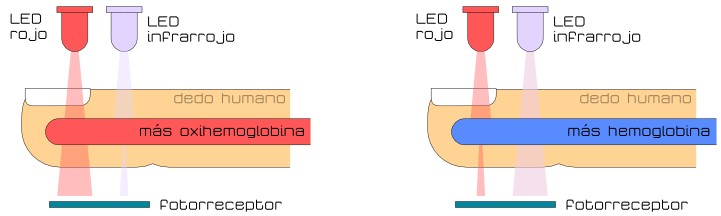
\includegraphics[width=0.9\linewidth]{img/funcionamiento-oxímetro-pulsómetro.png}
    \caption[Esquema de funcionamiento de un pulsioxímetro.]{Esquema de funcionamiento de un pulsioxímetro.\\ 
    Fuente: \cite{ventura2024monitorizacion}.}
    \label{fig:pulsioximetro}
\end{figure}

Los dispositivos portátiles o \textit{wearables} que incorporan esta tecnología se han popularizado como herramientas de cribado y autoseguimiento del sueño. Entre ellos se incluyen relojes inteligentes, anillos biométricos, bandas de muñeca y sensores integrados en colchones. Su funcionamiento se basa en la recolección de parámetros como el movimiento, la frecuencia cardíaca, la variabilidad del ritmo cardíaco, la temperatura corporal o la saturación de oxígeno. Entre los principales tipos de dispositivos destacan:

\begin{itemize}
    \item \textbf{Relojes inteligentes y pulseras de actividad:} como Fitbit, Garmin o Apple Watch, permiten registrar fases del sueño, ritmo cardíaco y actividad diaria. Su precisión es moderada y varía según el fabricante.
    \item \textbf{Anillos inteligentes:} como el \textit{Oura Ring}, combinan sensores de temperatura, frecuencia cardíaca y movimiento para analizar el sueño y la recuperación física.
    \item \textbf{Sensores bajo el colchón:} como el \textit{Withings Sleep Analyzer}, detectan ronquidos, movimientos y eventos respiratorios.
    \item \textbf{Pulsioxímetros nocturnos:} como el O2Ring, monitorizan continuamente la saturación de oxígeno y la frecuencia cardíaca durante el sueño mediante fotopletismografía.
\end{itemize} 
Aunque presentan limitaciones en la estimación de las fases del sueño o en la precisión de ciertos parámetros, su facilidad de uso y bajo coste los convierte en herramientas útiles para la detección preliminar de trastornos como el insomnio o la apnea del sueño.

\newpage
\textbf{O2Ring}

El \textbf{O2Ring} es un anillo inteligente desarrollado por la empresa \textit{\href{https://www.viatomtech.com/po2?lang=es}{Viatom}} que permite monitorizar de forma continua durante el sueño dos variables clave: la saturación de oxígeno en sangre (SpO\textsubscript{2}) y la frecuencia cardíaca. Su diseño compacto y cómodo lo convierte en una herramienta accesible para la detección domiciliaria de alteraciones respiratorias nocturnas, como apneas o desaturaciones.

Utiliza tecnología de \textbf{fotopletismografía (PPG)}, basada en la emisión de luz infrarroja y roja, que es absorbida de forma diferente por la hemoglobina oxigenada y desoxigenada. Esta propiedad permite estimar de manera precisa el porcentaje de oxígeno en sangre y la frecuencia cardíaca del usuario mientras duerme.

\begin{figure} [H]
    \centering
    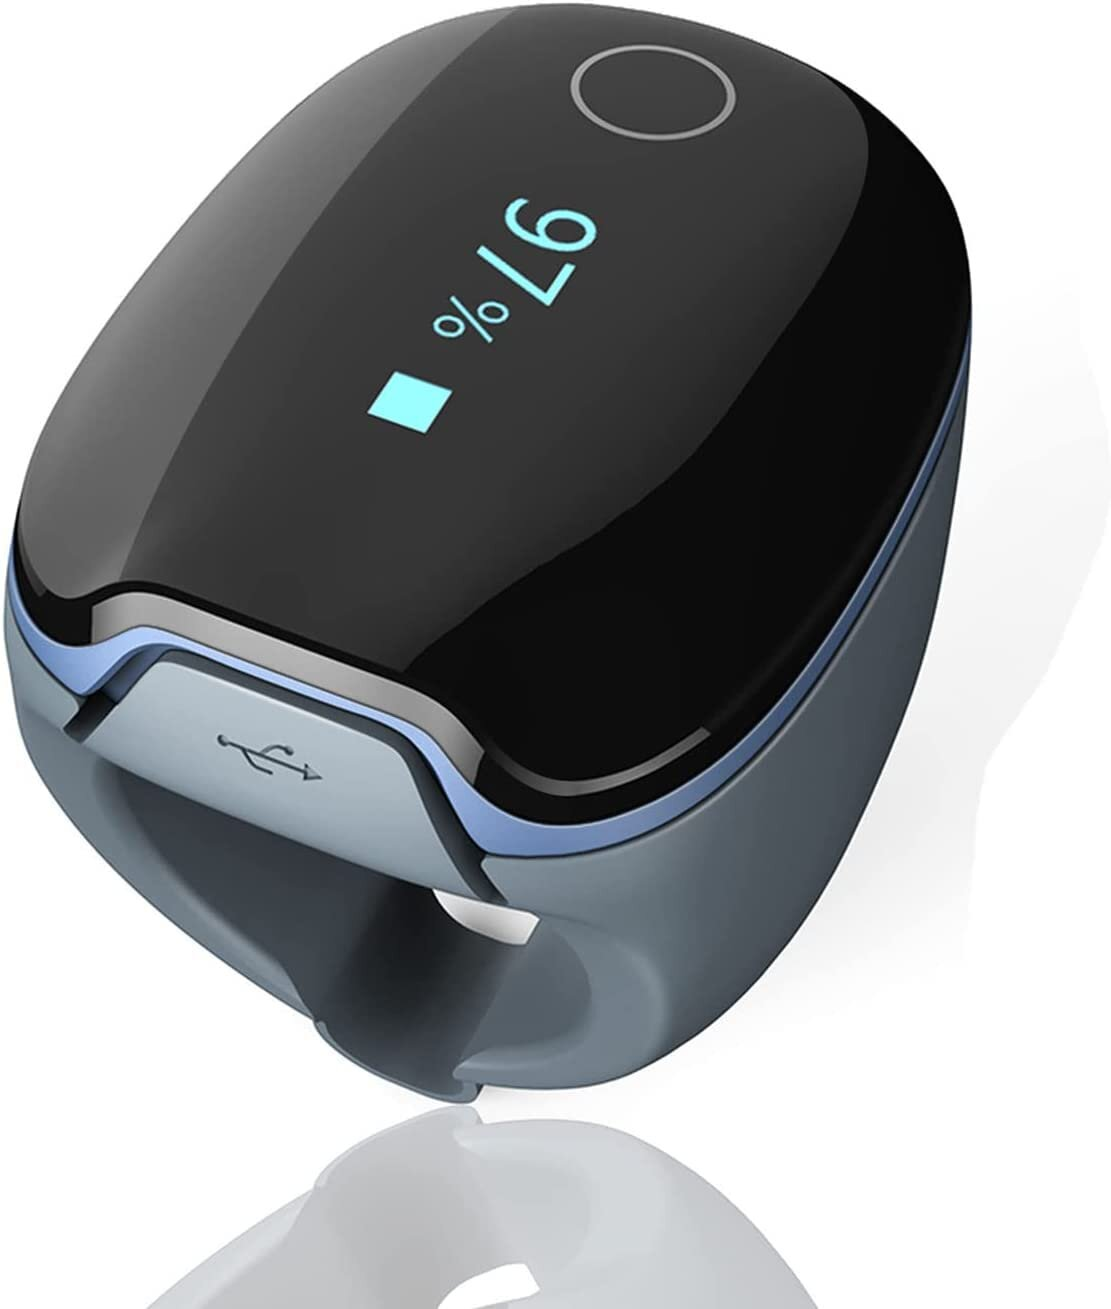
\includegraphics[width=0.25\linewidth]{img/o2ring.jpg}
    \caption[Dispositivo O2Ring de Viatom.]{Dispositivo O2Ring de Viatom. Fuente: \cite{o2ring_ifdesign}.}
    \label{fig:o2ring}
\end{figure}

Entre sus características principales destacan:
\begin{itemize}
    \item Registro continuo y no invasivo de SpO\textsubscript{2} y frecuencia cardíaca.
    \item Alertas por vibración ante desaturaciones significativas.
    \item Sincronización con apps móviles y exportación de informes en PDF o CSV.
    \item Generación de métricas como el índice de desaturación de oxígeno (ODI) o el tiempo con SpO\textsubscript{2} por debajo del 90\%.
\end{itemize}

A nivel clínico, el O2Ring se ha validado como herramienta útil en el \textit{screening}\footnote{El término \textit{screening} hace referencia a un proceso de cribado o detección precoz, que permite identificar posibles enfermedades en personas aparentemente sanas mediante pruebas rápidas, accesibles y no invasivas.} de apnea del sueño leve o moderada, especialmente en casos donde no se dispone de una polisomnografía completa. También permite un seguimiento longitudinal de pacientes y una evaluación complementaria a métodos tradicionales.

No obstante, presenta limitaciones: no ofrece información sobre las fases del sueño, ni detecta apneas centrales ni distingue entre tipos de eventos respiratorios. Por tanto, debe utilizarse como complemento y no como sustituto de un diagnóstico clínico completo.

En este trabajo, el O2Ring se ha utilizado como herramienta auxiliar para validar perfiles clínicos. Las métricas extraídas de sus informes (como caídas sostenidas de SpO$_2$, frecuencia cardíaca elevada y valores anómalos de ODI) permitieron reforzar la evaluación del modelo predictivo frente a situaciones clínicas reales.


\subsection{Cuestionarios Subjetivos}

\subsubsection{Índice de Calidad del Sueño de Pittsburgh (PSQI)}

El \textbf{Pittsburgh Sleep Quality Index (PSQI)} es un cuestionario ampliamente utilizado para evaluar la calidad subjetiva del sueño en el último mes. Consiste en 19 ítems agrupados en siete componentes: calidad subjetiva, latencia del sueño, duración, eficiencia, despertares nocturnos, uso de medicación y somnolencia diurna \cite{buysse1989pittsburgh}.

Su facilidad de aplicación y su validez en la detección de trastornos del sueño lo convierten en una herramienta útil tanto en investigación como en práctica clínica \cite{mollayeva2016pittsburgh}. Sin embargo, al basarse en autoinforme, puede estar sujeto a \textbf{sesgos de percepción} y variabilidad interindividual.

\subsubsection{Índice de Gravedad del Insomnio (ISI)}
El \textbf{Índice de Gravedad del Insomnio (ISI)} es un cuestionario diseñado específicamente para evaluar la severidad del insomnio. Se compone de siete ítems que valoran la dificultad para iniciar y mantener el sueño, la interferencia con la vida diaria y la preocupación del paciente por sus problemas de sueño \cite{ISI}.

El ISI es una herramienta eficaz para el diagnóstico y seguimiento del insomnio, aunque su uso es complementario a otros métodos, ya que no permite identificar causas orgánicas subyacentes.

\subsubsection{Escala de Somnolencia de Epworth (ESS)}
La \textbf{Escala de Somnolencia de Epworth (ESS)} mide la propensión del individuo a quedarse dormido en diversas situaciones diurnas, como leer, ver televisión o viajar como pasajero. Su puntuación permite detectar somnolencia excesiva, siendo útil en la evaluación de apnea del sueño y narcolepsia \cite{epworth}.

Si bien es una herramienta sencilla y fiable, la ESS es una medida subjetiva y no sustituye a pruebas objetivas como la PSG o el Test de Latencia Múltiple del Sueño (MSLT) \cite{pedrozo2020estructura}.

\subsubsection{Escala de Somnolencia de Stanford (SSS)}
La \textbf{Escala de Somnolencia de Stanford (SSS)} permite medir el nivel de alerta en distintos momentos del día mediante una escala de 1 a 7. Se utiliza en estudios sobre privación de sueño y trastornos de vigilia \cite{stanford}. Aunque es útil para evaluar la somnolencia en tiempo real, su aplicación es más limitada en comparación con otras herramientas subjetivas de evaluación del sueño.

\noindent
En conjunto, las herramientas descritas conforman un ecosistema amplio para la evaluación del sueño, que va desde técnicas clínicas de alta precisión hasta métodos accesibles y subjetivos. En este trabajo, se ha optado por un enfoque centrado en datos autodeclarados y medidas clínicas básicas, complementado con la validación externa mediante pulsioximetría. Esta combinación busca maximizar la accesibilidad del sistema predictivo sin comprometer su rigor diagnóstico.


\section{Aprendizaje automático (Machine Learning) en medicina}

El aprendizaje automático (Machine Learning, ML) es una rama de la inteligencia artificial que desarrolla algoritmos capaces de aprender patrones a partir de datos y realizar predicciones o decisiones sin estar explícitamente programados para cada tarea. En el contexto médico, su uso ha crecido de forma exponencial debido al aumento del volumen de datos clínicos disponibles y a la necesidad de herramientas que faciliten su análisis e interpretación.

Entre sus principales aplicaciones en el ámbito de la salud destacan:

\begin{itemize}
    \item \textbf{Diagnóstico asistido}: identificación de enfermedades a partir de imágenes médicas, señales fisiológicas o datos clínicos estructurados\footnote{\href{https://doi.org/10.1038/s41591-018-0337-2}{Guía para el aprendizaje profundo en el ámbito sanitario.}}.
    \item \textbf{Pronóstico de enfermedades}: predicción de la evolución clínica de un paciente, el riesgo de complicaciones o la respuesta esperada a un tratamiento.
    \item \textbf{Medicina personalizada}: adaptación de estrategias terapéuticas en función de las características genéticas, clínicas o conductuales del paciente.
    \item \textbf{Gestión hospitalaria}: optimización de flujos de trabajo, recursos sanitarios y toma de decisiones administrativas.
\end{itemize}

El uso de modelos de ML en medicina plantea, no obstante, desafíos importantes. Entre ellos destacan la necesidad de trabajar con datos clínicos de calidad, garantizar la equidad en las predicciones para evitar sesgos, y asegurar que los modelos sean interpretables, especialmente en entornos clínicos donde las decisiones deben ser justificadas de forma transparente.


\subsection{Modelos predictivos}
Los modelos predictivos son herramientas estadísticas y computacionales que permiten anticipar eventos futuros o clasificar instancias a partir de patrones aprendidos de datos. En el ámbito de la salud, estos modelos se emplean para prever la aparición de enfermedades, evaluar riesgos clínicos y apoyar la toma de decisiones médicas, especialmente en contextos como la predicción de trastornos del sueño.

A continuación, se describen algunos de los modelos más empleados en aprendizaje automático supervisado, todos ellos utilizados en este trabajo para predecir la presencia de trastornos del sueño a partir de variables clínicas y de estilo de vida.


\subsubsection{Regresión Logística}
La \textbf{regresión logística} es un modelo de clasificación (binaria o multiclase) que estima la probabilidad de pertenencia a una clase utilizando la función sigmoide. Se basa en la regresión lineal, pero transforma su salida en valores entre 0 y 1 mediante la función logística, que son interpretables como probabilidades:


\begin{equation}
    P(Y=1 \mid X)=\frac{1}{1+e^{-\left(\beta_{0}+\beta_{1} X_{1}+\ldots+\beta_{n} X_{n}\right)}}
\end{equation}
Donde $\beta$ representa los coeficientes del modelo, estimados mediante máxima verosimilitud. La regresión logística se utiliza ampliamente en medicina por su bajo coste computacional, facilidad de implementación e interpretabilidad de los resultados \cite{datatab_logistic_regression}.

\begin{figure}[H]
    \centering
    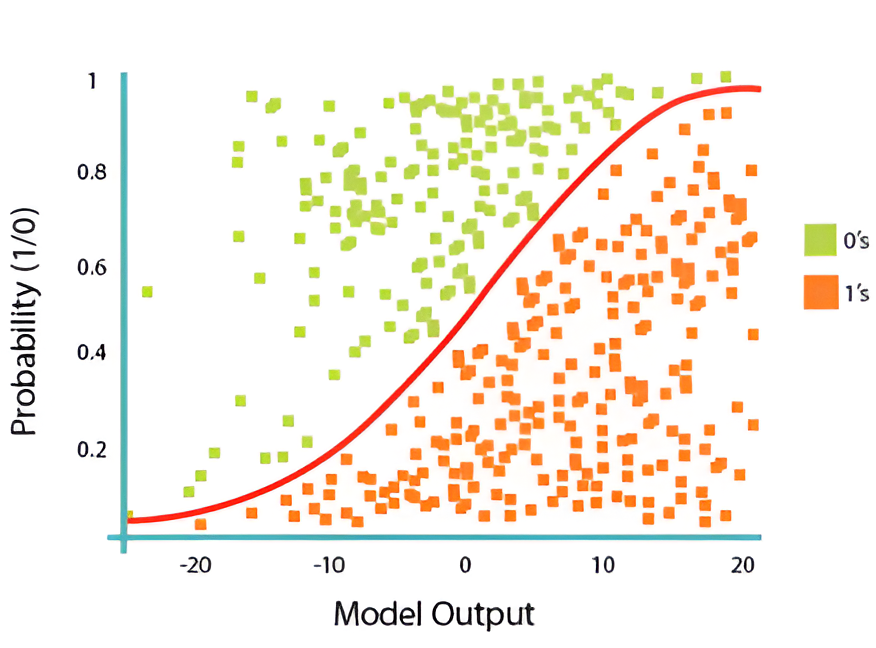
\includegraphics[width=0.5\linewidth]{img/regresionLogistica.png}
    \caption[Representación de la curva sigmoide en un modelo de regresión logística binaria.]{Representación de la curva sigmoide en un modelo de regresión logística binaria. Fuente: \cite{rafael2024ml}.}
    \label{fig:regresion_logistica}
\end{figure}

Su transparencia y la interpretación directa de los coeficientes hacen que la regresión logística sea especialmente adecuada en entornos clínicos donde se requiere justificar cada decisión de forma comprensible para el personal médico.

\subsubsection{Árboles de Decisión}

Los árboles de decisión dividen el espacio de características en regiones homogéneas mediante divisiones sucesivas. Cada nodo representa una condición sobre una variable, y las ramas conducen a clases específicas. El criterio de impureza más utilizado es el índice de Gini:


\begin{equation}
    Gini=1-\sum_{i=1}^{C} p_{i}^{2}
\end{equation}
 
donde $p_i$ es la proporción de observaciones de la clase $i$ en el nodo. Este modelo es especialmente útil en medicina por su capacidad explicativa y visual. Sin embargo, sufre de sobreajuste, por lo que suele combinarse con técnicas de ensamblado como Random Forest \cite{datacamp_decision_tree}.

\begin{figure}[H]
    \centering
    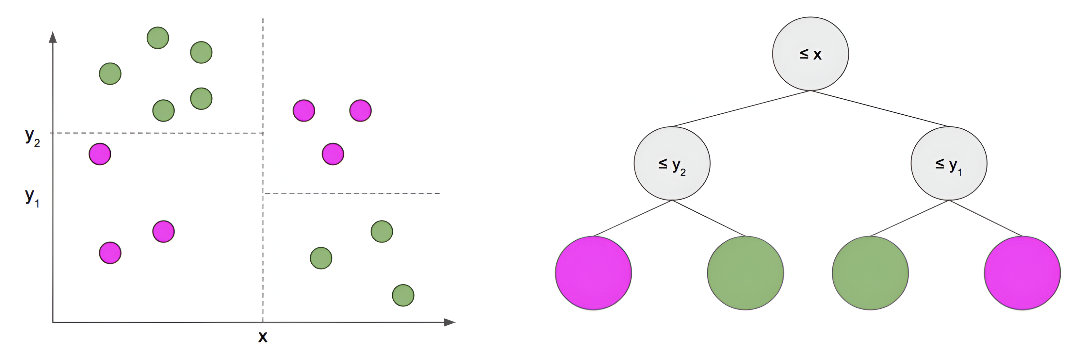
\includegraphics[width=0.7\linewidth]{img/decision_tree.png}
    \caption[Ejemplo ilustrativo del funcionamiento de un árbol de decisión.]{Ejemplo ilustrativo del funcionamiento de un árbol de decisión. Fuente: \cite{orellana2018arboles}.}
    \label{fig:decision-tree}
\end{figure}

Pese a su sencillez, los árboles de decisión ofrecen una visualización directa del proceso de toma de decisiones, siendo útiles tanto en fase exploratoria como en modelos base para técnicas más robustas como Random Forest.

\subsubsection{Máquinas de Vectores de Soporte}

Las \textbf{SVM} son modelos supervisados que buscan un hiperplano óptimo que separe las clases maximizando el margen entre ellas. Su formulación para el caso lineal es:


\begin{equation}
    \max _{\mathbf{w}, b} \frac{1}{\|\mathbf{w}\|} \quad \text { sujeto a } \quad y_{i}\left(\mathbf{w} \cdot \mathbf{x}_{i}+b\right) \geq 1, \forall i
\end{equation}
Donde w es el vector normal al hiperplano y b es el sesgo. 

En casos no lineales, se emplean funciones kernel (como RBF) para proyectar los datos a un espacio de mayor dimensión. Las SVM son ampliamente utilizadas en biomedicina para tareas de clasificación sobre señales fisiológicas \cite{ibm_svm}. 

\begin{figure}[H]
    \centering
    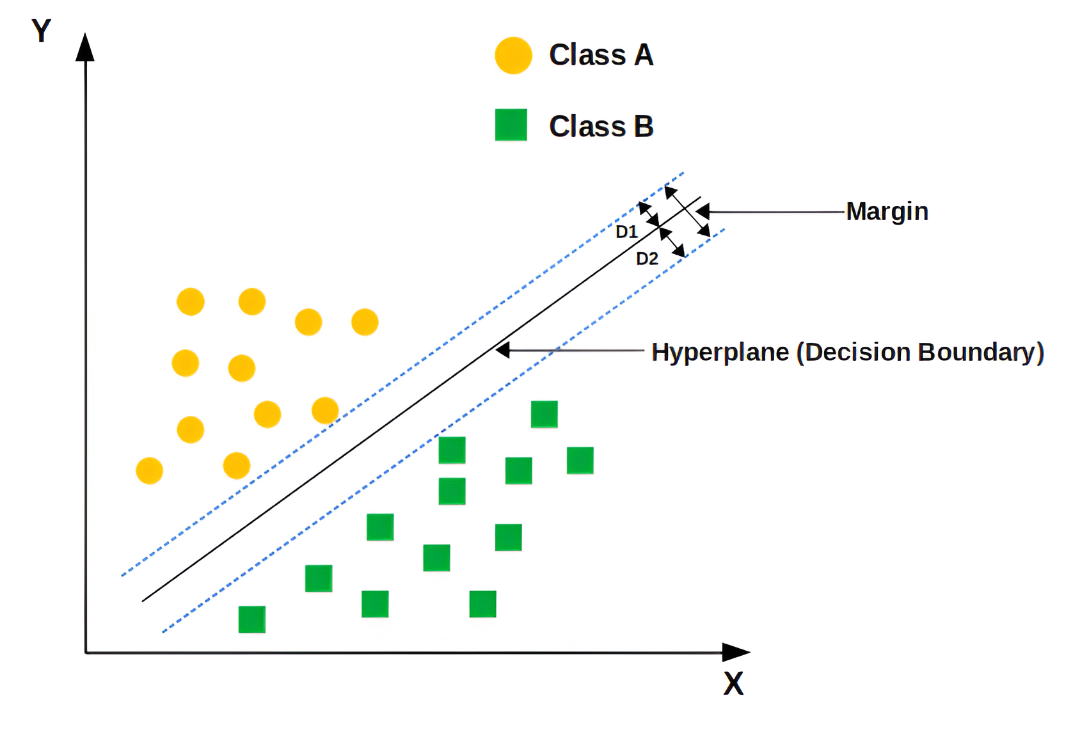
\includegraphics[width=0.8\linewidth]{img/svm.png}
    \caption[Imagen representativa del funcionamiento de SVM.]{Imagen representativa del funcionamiento de SVM.\\ Fuente: \cite{mehta2021svm}.}
    \label{fig:svm}
\end{figure}

Sin embargo, su coste computacional aumenta significativamente con el tamaño del conjunto de entrenamiento y la necesidad de ajustar adecuadamente el kernel y sus parámetros puede limitar su aplicabilidad práctica en tiempo real.

\subsubsection{Perceptrón Multicapa (MLP)}
El\textbf{ MLP} es un tipo de red neuronal que consta de una capa de entrada, una o más ocultas y una de salida. Cada neurona aplica una función de activación a una combinación ponderada de las entradas:

\begin{equation}
    h_{j}=f\left(\sum_{i=1}^{n} w_{j i} x_{i}+b_{j}\right)
\end{equation}
Donde w\textsubscript{ji }son los pesos sinápticos y b\textsubscript{j} es el sesgo. 

Este modelo se entrena por retropropagación del error, utilizando algoritmos de descenso de gradiente. En medicina, se emplea para la clasificación de EEG, oximetría y otros biomarcadores \cite{ibm_mlp}.

\begin{figure}[H]
    \centering
    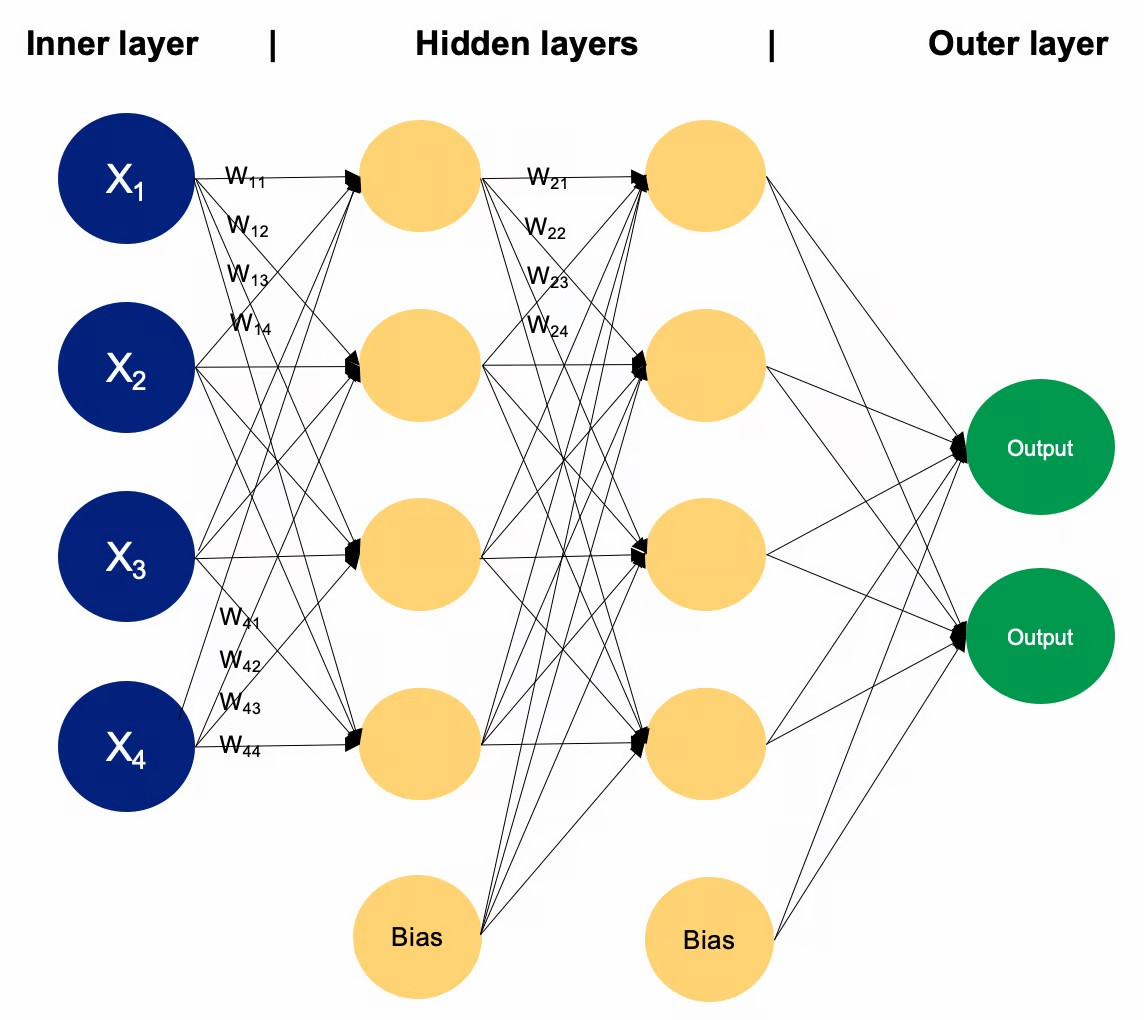
\includegraphics[width=0.8\linewidth]{img/mlp.jpg}
    \caption[Imagen representativa del funcionamiento de MLP.]{Imagen representativa del funcionamiento de MLP.\\ Fuente: \cite{mlp}.}
    \label{fig:mlp}
\end{figure}

\subsubsection{Random Forest}
\textbf{Random Forest} es un algoritmo de ensamblado que combina múltiples árboles de decisión entrenados con subconjuntos aleatorios del conjunto de datos y características (bagging). La predicción final se obtiene por votación mayoritaria:

\begin{equation}
    \hat{y}=\operatorname{modo}\left(T_{1}(x), T_{2}(x), \ldots, T_{n}(x)\right)
\end{equation}
Donde T\textsubscript{i}(x) es la predicción del i-ésimo árbol. Este enfoque mejora la generalización y reduce el sobreajuste. En medicina, ha demostrado buen rendimiento en la detección de apnea del sueño y otras condiciones clínicas complejas \cite{ibm_random_forest}.

\begin{figure}[H]
    \centering
    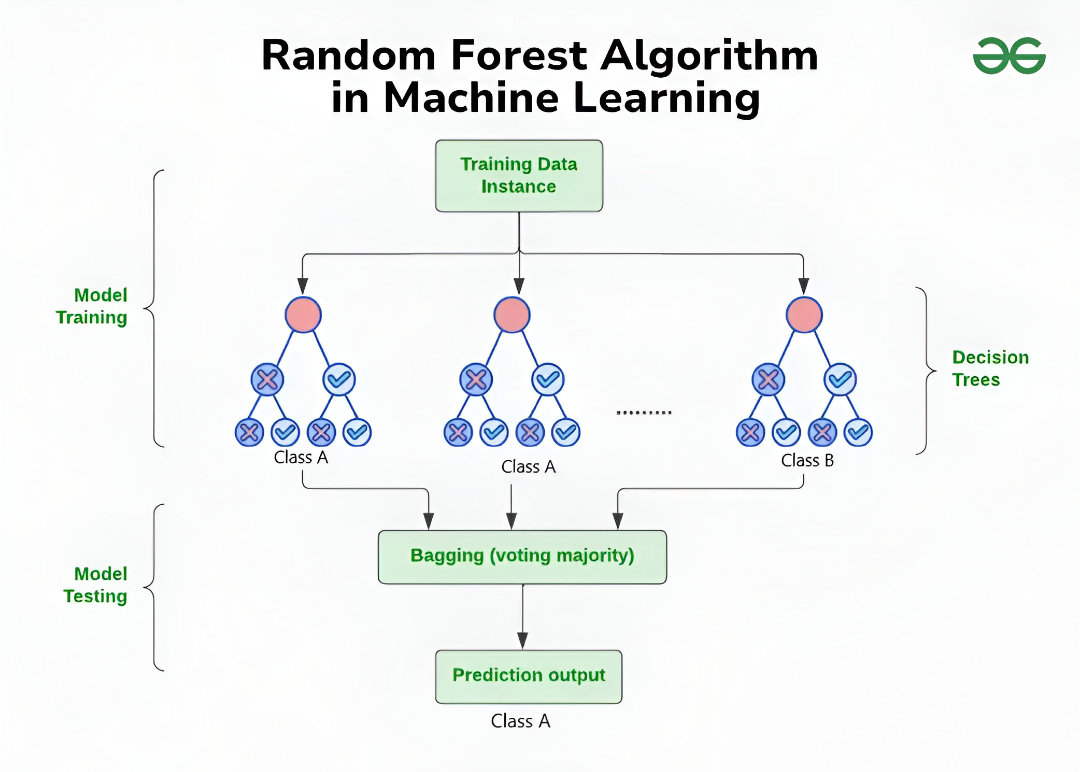
\includegraphics[width=0.8\linewidth]{img/randomForest.jpg}
    \caption[Imagen representativa del funcionamiento de Random Forest.]{Imagen representativa del funcionamiento de Random Forest. Fuente: \cite{random_forest}.}
    \label{fig:rf}
\end{figure}
Su robustez frente al sobreajuste y su capacidad para manejar datos heterogéneos lo convierten en un candidato idóneo para modelos clínicos en los que se combinan variables fisiológicas, demográficas y del estilo de vida, como en el presente trabajo.

\section{Desbalanceo de clases y técnica SMOTE}

En problemas de clasificación médica, especialmente en contextos de cribado o detección precoz, es habitual que algunas clases, como la presencia de una patología, estén infrarrepresentadas respecto a la clase mayoritaria. En el caso de los trastornos del sueño, por ejemplo, suele haber más registros de personas sin patología que de pacientes con insomnio o apnea, lo que dificulta que los modelos aprendan patrones representativos de las clases minoritarias.

Este desequilibrio puede inducir una falsa sensación de buen rendimiento basada únicamente en la exactitud global, mientras que el modelo falla sistemáticamente en identificar los casos clínicamente relevantes (baja sensibilidad).

Para mitigar este problema, una de las técnicas más utilizadas es el \textit{Synthetic Minority Over-sampling Technique} (SMOTE), propuesta por \cite{chawla2002smote}. SMOTE genera nuevas instancias sintéticas de la clase minoritaria mediante interpolación entre ejemplos reales, evitando el sobreajuste que provoca el simple duplicado de muestras. De este modo, se logra una representación más equilibrada del espacio de características.

Su aplicación ha demostrado mejorar métricas clave como la sensibilidad y el F1-score en tareas de clasificación médica sobre conjuntos de datos desbalanceados \cite{fernandez2018smote}. No obstante, en problemas multiclase puede introducir ruido si las fronteras entre clases están poco definidas, por lo que su uso debe ser evaluado cuidadosamente.

En este trabajo, se ha evaluado el impacto de aplicar SMOTE en combinación con distintos algoritmos, comparando su rendimiento frente a versiones no balanceadas del modelo. Se ha observado una mejora significativa en la sensibilidad de las clases minoritarias (insomnio y apnea), lo que justifica su uso controlado en la fase de entrenamiento.

Una vez mitigado el desbalance entre clases, resulta fundamental garantizar que las decisiones del modelo sean comprensibles y justificables desde un punto de vista clínico. Por este motivo, se han aplicado técnicas de interpretabilidad como SHAP.

\section{Interpretabilidad del modelo: SHAP}

En el desarrollo de modelos predictivos aplicados a la medicina, la interpretabilidad es una condición indispensable para garantizar transparencia diagnóstica y confianza por parte de los profesionales. A diferencia de los modelos lineales, muchas técnicas avanzadas de aprendizaje automático —como los ensamblados o las redes neuronales— actúan como cajas negras, dificultando la explicación de las decisiones individuales del sistema.

Entre las técnicas más consolidadas para interpretar este tipo de modelos destaca SHAP (\textit{SHapley Additive exPlanations}), una metodología basada en los valores de Shapley de la teoría de juegos cooperativos \cite{shap}. SHAP permite descomponer cada predicción en contribuciones atribuibles a cada variable de entrada, cuantificando la influencia de cada una sobre el resultado final.

Las principales ventajas de SHAP en contextos clínicos incluyen:

\begin{itemize}
  \item \textbf{Validación del modelo:} permite verificar que las decisiones se basan en relaciones clínicas coherentes y no en correlaciones espurias.
  \item \textbf{Generación de confianza:} facilita la aceptación del sistema por parte de los profesionales, al ofrecer una explicación intuitiva y detallada de cada recomendación.
  \item \textbf{Detección de sesgos:} ayuda a identificar variables con un impacto indebido sobre la salida del modelo, revelando posibles fuentes de discriminación o error.
  \item \textbf{Medicina personalizada:} permite adaptar la interpretación del modelo al perfil específico de cada paciente, favoreciendo decisiones individualizadas.
\end{itemize}

En el presente trabajo, SHAP se ha utilizado para analizar tanto la importancia media de cada predictor como su contribución específica a cada observación. Por ejemplo, en ciertos perfiles clínicos simulados, SHAP mostró que variables como la ocupación laboral, el nivel de estrés y la duración del sueño tenían más peso que el IMC en la predicción de insomnio. Esta capacidad de explicación local y global convierte a SHAP en una herramienta clave para garantizar la trazabilidad y justificación de las decisiones clínicas basadas en el modelo.


\section{Aplicaciones web interactivas en Ciencia de Datos}
En el contexto del aprendizaje automático y la ingeniería biomédica, las aplicaciones web interactivas permiten acercar los modelos predictivos al usuario final de manera accesible, visual y funcional. Estas herramientas actúan como una capa de interfaz entre los algoritmos complejos desarrollados durante la fase de entrenamiento y el profesional sanitario o paciente que desea obtener información personalizada a partir de ellos.

\subsection{Interfaz como puente entre el modelo y el usuario}
Una aplicación interactiva permite al usuario introducir variables relevantes (como edad, presión arterial, nivel de estrés, calidad del sueño, etc.) y recibir una predicción automática y explicable generada por el modelo, sin necesidad de conocimientos técnicos. Esta predicción puede estar acompañada de explicaciones visuales, indicadores de riesgo o recomendaciones, lo que mejora la interpretabilidad de los resultados y su utilidad clínica.

En ingeniería de la salud, estas herramientas tienen un alto potencial: pueden contribuir al cribado poblacional, al apoyo en la toma de decisiones clínicas o al autocuidado en poblaciones con riesgo de enfermedades crónicas. La posibilidad de utilizar estas aplicaciones desde cualquier dispositivo con conexión a internet facilita, además, la democratización del acceso a tecnologías basadas en inteligencia artificial.

\subsection{Streamlit como herramienta de desarrollo}
Streamlit es un framework de código abierto en Python diseñado específicamente para crear aplicaciones web interactivas orientadas a la ciencia de datos y el aprendizaje automático \cite{streamlit}. Su sintaxis sencilla permite transformar scripts de análisis en interfaces web funcionales sin necesidad de conocimientos avanzados de desarrollo frontend.

Entre sus características principales destacan:
\begin{itemize}
    \item \textbf{Facilidad de uso}: permite crear interfaces web con pocas líneas de código.
    \item \textbf{Compatibilidad}: se integra de forma nativa con bibliotecas populares como \textit{Pandas}, \textit{scikit-learn}, \textit{Matplotlib} o \textit{SHAP}.
    \item \textbf{Interactividad}: permite actualizar los resultados en tiempo real conforme el usuario introduce nuevos datos.
\end{itemize}

Gracias a estas ventajas, Streamlit se presenta como una solución ideal para prototipado rápido, aplicaciones ligeras o proyectos académicos. En el presente trabajo, se ha utilizado para desarrollar una aplicación interactiva que permite introducir datos personales, realizar una predicción automática del tipo de trastorno del sueño (si lo hubiera) y visualizar las variables que han contribuido a dicha decisión. Esta estrategia refuerza la transparencia y confiabilidad del sistema, facilitando su adopción tanto por profesionales clínicos como por usuarios finales sin conocimientos de programación.

El desarrollo de esta interfaz mediante Streamlit ha sido clave para trasladar el modelo predictivo desde un entorno experimental hacia una herramienta funcional, explicable y accesible, en línea con las necesidades de los sistemas de salud actuales.


\section{Estado del arte y trabajos relacionados}

\subsection{Aplicación del aprendizaje automático al estudio del sueño}

En los últimos años, el uso de modelos de aprendizaje automático (ML) para el estudio del sueño ha cobrado gran relevancia, tanto en el ámbito clínico como en el desarrollo de soluciones portables y accesibles. Estas técnicas permiten desarrollar sistemas predictivos no invasivos, capaces de analizar grandes volúmenes de datos clínicos y autodeclarados con fines de cribado o apoyo diagnóstico.

Ha et al. (2023) desarrollaron un modelo basado en \textit{XGBoost} para predecir la presencia de apnea del sueño (OSA), insomnio o COMISA, utilizando variables clínicas y autodeclaradas. La herramienta, denominada \textit{SLEEPS}, alcanzó un AUC superior a 0.89 en todos los modelos, y fue desplegada como una aplicación web accesible, integrando explicaciones mediante \textit{SHAP} \cite{ha2023sleeps}. Este enfoque es conceptualmente similar al adoptado en el presente trabajo, aunque aquí se ha optado por un modelo Random Forest con calibración, interpretabilidad visual y exportación de informes.

Otro estudio relevante es el de Alazaidah et al. (2023), que realizaron una comparación exhaustiva entre modelos de regresión y clasificación aplicados a la predicción de trastornos del sueño. Su análisis evidencia el potencial del aprendizaje automático para detectar condiciones como insomnio o apnea mediante variables clínicas, sociodemográficas y de estilo de vida \cite{alazaidah2023potential}.


\subsection{Modelos centrados en la predicción de calidad del sueño}

Además de los enfoques clínicos tradicionales, diversos estudios han explorado la predicción de la calidad del sueño desde una perspectiva continua, empleando dispositivos portátiles y variables fisiológicas.

Sathyanarayana et al. (2016) desarrollaron modelos de redes neuronales para predecir la calidad del sueño (medida en términos de eficiencia) utilizando únicamente los datos recogidos durante el día por dispositivos portátiles. Este enfoque destaca por evitar la necesidad de medir parámetros nocturnos, y por lograr resultados robustos en tareas de clasificación binaria entre “sueño bueno” y “sueño pobre” \cite{sathyanarayana2016sleep}.

De forma similar, Kilic et al. (2023) entrenaron modelos de \textit{convolutional neural networks} y \textit{ensemble learning} utilizando el conjunto de datos NetHealth, que incluye registros de 698 estudiantes universitarios. Obtuvieron resultados prometedores en la clasificación binaria de calidad del sueño, utilizando variables como la actividad física, el nivel de estrés y datos recogidos por sensores portátiles. Estos hallazgos destacan el potencial de los enfoques basados en dispositivos cotidianos para aplicaciones de salud digital \cite{wearablesCNN}.

En un contexto más fisiológico, Di Credico et al. (2024) utilizaron biofeedback (variabilidad de la frecuencia cardíaca, temperatura cutánea) para estimar la calidad del sueño, validándolo contra el índice de Pittsburgh (PSQI). Sus resultados confirmaron que es posible aproximar la calidad subjetiva del sueño mediante parámetros fácilmente medibles, lo cual apoya la base del presente trabajo, basado también en datos autodeclarados y clínicos \cite{di2024predicting}.

\subsection{Interpretabilidad y herramientas explicables}

Uno de los retos más relevantes en el uso de modelos de ML en medicina es la necesidad de interpretabilidad. Ahadian et al. (2024) propusieron un modelo híbrido (LSTM + TCN + Transformer) para predecir trastornos del sueño, complementado con explicaciones SHAP y contrafactuales. Su trabajo demuestra que es posible combinar precisión técnica con trazabilidad clínica \cite{ahadian2024explainable}.

En este trabajo, se ha seguido una filosofía similar al incorporar SHAP tanto en la interpretación global como individual del modelo. Esta integración permite justificar cada predicción y y presentarla de forma comprensible y justificable ante profesionales clínicos o incluso pacientes.

\subsection{Aplicaciones interactivas y despliegue accesible}

El uso de interfaces interactivas para la predicción personalizada ha sido ya validado en estudios como el de Ha et al. (2023), que despliega su modelo mediante una herramienta web que incluye visualizaciones y explicaciones automáticas. De forma complementaria, Espie et al. (2012) demostraron que una aplicación basada en terapia cognitivo-conductual (\textit{Sleepio}) era capaz de mejorar significativamente los síntomas de insomnio en ensayos clínicos aleatorizados \cite{espie2012sleepio}.

Este tipo de plataformas no solo permiten hacer llegar la predicción a la población general, sino que también facilitan el seguimiento clínico o el autodiagnóstico responsable.

El presente trabajo se sitúa en esta línea, pero con un enfoque distinto: se ha desarrollado una aplicación ligera y accesible mediante \textit{Streamlit}, que combina predicción multiclase personalizada, visualización explicativa mediante \textit{SHAP} y generación automática de informes PDF con orientación clínica. A diferencia de otras plataformas centradas en intervención terapéutica, esta herramienta busca facilitar el cribado inicial y la comunicación clara de los resultados, sin requerir conocimientos técnicos por parte del usuario final.


\subsection{Modelos basados en señales fisiológicas y pulsioximetría}

Varios trabajos recientes han explorado la posibilidad de detectar trastornos del sueño, especialmente apnea obstructiva, a partir de señales fisiológicas obtenidas mediante pulsioximetría o sensores biométricos portátiles. Estos enfoques buscan alternativas menos invasivas que la polisomnografía, apoyándose en señales como la saturación de oxígeno (SpO$_2$) y la frecuencia cardíaca (FC) registradas durante el sueño.

Gutiérrez-Tobal et al. (2020) desarrollaron un sistema basado en aprendizaje automático para la detección de apnea del sueño exclusivamente a partir de la señal de SpO$_2$. Empleando un conjunto amplio de características estadísticas y morfológicas extraídas de la pulsioximetría nocturna, validadas frente a polisomnografía, logrando una alta precisión y sensibilidad \cite{gutierrez2020apnea}.


Por otro lado, Casal et al. (2024) plantearon un enfoque aún más avanzado, integrando redes neuronales de tipo TCN (Temporal Convolutional Networks) y capas Transformer. Utilizaron como entrada señales longitudinales de pulsioximetría y aplicaron técnicas de atención para destacar los intervalos temporales más relevantes. Su modelo logró una discriminación efectiva entre sujetos control y pacientes con apnea, proponiendo además un marco explicable mediante visualización de pesos de atención \cite{casal2021tcn}.

Estos estudios refuerzan el valor de incluir variables fisiológicas reales en el desarrollo de modelos explicables. Aunque el presente trabajo no integra todavía señales en tiempo real, se ha realizado una validación preliminar con el O2Ring, sentando las bases para una futura evolución del sistema hacia una monitorización continua y más precisa de la salud del sueño.

\noindent
Los conceptos revisados en este capítulo proporcionan el marco teórico necesario para comprender los fundamentos clínicos, técnicos y computacionales del sistema desarrollado. Desde los trastornos del sueño y sus variables asociadas hasta las técnicas de aprendizaje automático, interpretabilidad y despliegue interactivo, todos los elementos descritos se integran en el diseño de un modelo predictivo explicable y accesible. En el siguiente capítulo se detallan las fases metodológicas llevadas a cabo para su implementación, evaluación y validación práctica.

\capitulo{4}{Metodología}
\label{cap:metodologia}


La metodología seguida en este proyecto abarca todas las fases del desarrollo de un sistema predictivo de trastornos del sueño, con un enfoque ingenieril aplicado al ámbito clínico, que prioriza tanto la utilidad predictiva como la interpretabilidad. Se parte del tratamiento inicial de los datos, pasando por la evaluación y selección del modelo más adecuado, hasta el despliegue en una aplicación interactiva accesible para profesionales sanitarios o usuarios interesados. A continuación, se describen en detalle las etapas y técnicas empleadas.

\section{Desarrollo del modelo predictivo}

Para la implementación del modelo predictivo y su posterior integración en una aplicación interactiva, se utilizaron diversas herramientas y tecnologías que permitieron abarcar el proyecto desde el tratamiento de datos hasta el desarrollo de la interfaz.

Además de buscar un alto rendimiento estadístico, el objetivo fue desarrollar un sistema útil en el contexto clínico, capaz de proporcionar predicciones explicables sobre la presencia o ausencia de trastornos del sueño, facilitando su uso por parte de profesionales o usuarios sin conocimientos técnicos.

A continuación, se describen en detalle las etapas de análisis, entrenamiento y evaluación del sistema.


\subsection{Descripción de los datos}
El modelo predictivo desarrollado en este proyecto se ha basado en un conjunto de datos de acceso público, descargado de la plataforma \textbf{\href{https://www.kaggle.com/}{Kaggle}},  especializada en ciencia de datos y aprendizaje automático. El dataset seleccionado, titulado Sleep Health and Lifestyle Dataset\footnote{Dataset seleccionado: \cite{alnour2024kaggle}}, proporciona información sociodemográfica, clínica y de hábitos de vida de un total de 374 individuos.

Este conjunto de datos tiene como finalidad facilitar el estudio computacional de los principales trastornos del sueño mediante el análisis conjunto de factores personales, fisiológicos y conductuales, ofreciendo así una perspectiva multidimensional alineada con enfoques clínicos actuales.

Las variables incluidas en el conjunto de datos se pueden agrupar de la siguiente manera:
\begin{itemize}
    \item \textbf{Variables demográficas:}
\begin{itemize}
    \item Age: edad del paciente, expresada en años.
    \item Gender: género biológico, bien sea masculino o femenino (Male/Female).
    \item \textit{Occupation:} ocupación laboral principal (ingeniero, médico, representante de ventas...).
\end{itemize}

\item  \textbf{Variables clínicas:}
\begin{itemize}
    \item \textit{Blood Pressure}: presión arterial registrada en formato sistólica/diastólica, medida en mmHg ("120/80").
    \item  \textit{Heart Rate}: frecuencia cardíaca en reposo, representada en latidos por minuto.
    \item  \textit{BMI Category}: clasificación del índice de masa corporal (Underweight, Normal, Overweight, Obese)
\end{itemize}

  \item \textbf{Variables conductuales y de estilo de vida:}
\begin{itemize}
    \item Sleep Duration: duración media del sueño, en horas.
\item Quality of Sleep: valoración subjetiva de la calidad del sueño, incluida en una escala comprendida entre el 1 y el 10.
\item \textit{Stress Level}: nivel de estrés al que se ve sometido el paciente, percibido por él mismo. Representado en una escala del 1 a 10.
\item \textit{Physical Activity Level}: nivel de actividad física semanal (valor de 0 a 100). 
\item \textit{Daily Steps}: número medio de pasos diarios.
\end{itemize}
\item \textbf{Variable objetivo (target):}
\begin{itemize}
    \item \textit{Sleep Disorder}: clasificación del trastorno del sueño, categorizado en tres clases:
    \begin{itemize}
        \item \textit{None}: sin trastorno diagnosticado.
        \item \textit{Insomnia}: diagnóstico de insomnio.
        \item \textit{Sleep Apnea}: diagnóstico de apnea del sueño.
    \end{itemize}
\end{itemize}
\end{itemize}

El dataset original se encuentra en formato CSV (valores separados por comas) y fue tratado íntegramente en \textbf{Python}, utilizando librerías especializadas como \textbf{Pandas} y \textbf{NumPy} para su carga, transformación, análisis y modelado.

Aunque el conjunto de datos presenta limitaciones propias de los datos sintéticos o autodeclarados (como posibles sesgos o simplificaciones de la realidad clínica), su estructura es adecuada para la experimentación y la validación de metodologías de aprendizaje automático en el ámbito de la salud.

El conjunto de datos utilizado puede consultarse en el siguiente enlace: 
\href{https://www.kaggle.com/code/alnourabdalrahman9/sleeping-disorders-detection-outliers-removal/input}{\texttt{Sleep\_health\_and\_lifestyle\_dataset.csv}.}

\subsection{Carga y descripción inicial del conjunto de datos}

El archivo original fue cargado en un entorno de \href{file://C:/Users/Marina/OneDrive\%20-\%20Universidad\%20de\%20Burgos/Escritorio/TFG-Marina-Martin/notebooks/TFG3-Marina.ipynb}{Jupyter Notebook} mediante la librería \textbf{Pandas}, utilizando estructuras tipo \textbf{DataFrame}. Esta organización permitió realizar de forma eficiente operaciones de filtrado, transformación y exploración de las distintas variables.

\begin{figure}[H]
    \centering
    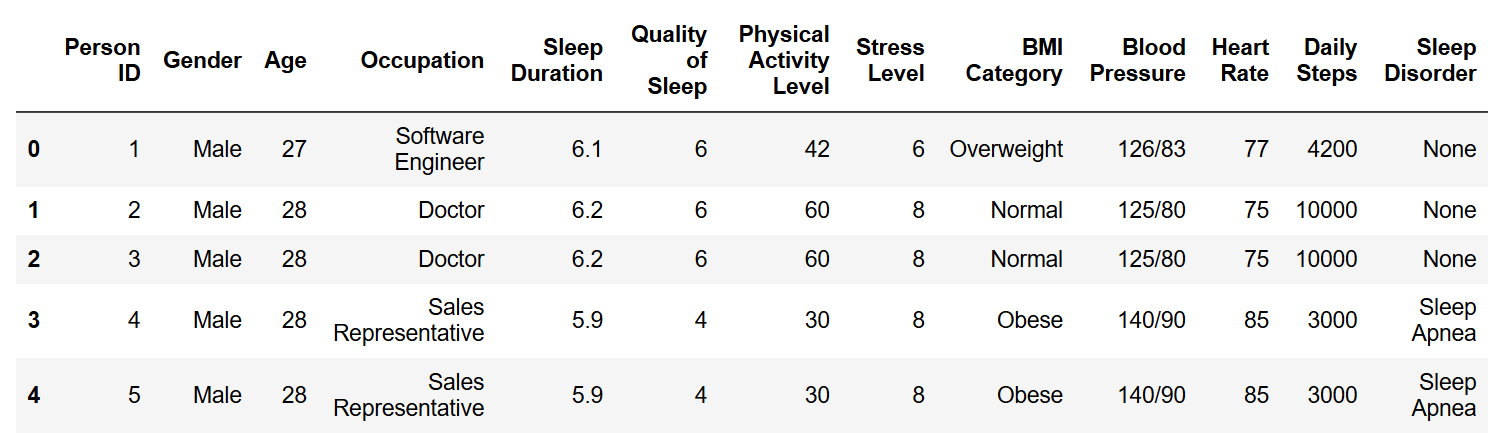
\includegraphics[width=1\linewidth]{img/datasetInicial.png}
    \caption{Dataset inicial.}
    \label{fig:dataset-inicial}
\end{figure}

A continuación se llevó a cabo una revisión estructural del dataset, aplicando distintos métodos de inspección:


\begin{itemize}
    \item \textbf{Tipos de datos:} se utilizó el método \texttt{df.info()} para verificar los tipos de datos de cada columna. Se identificaron 13 columnas: 8 numéricas y 5 categóricas (tipo \texttt{object}).

    \begin{figure}[H]
        \centering
        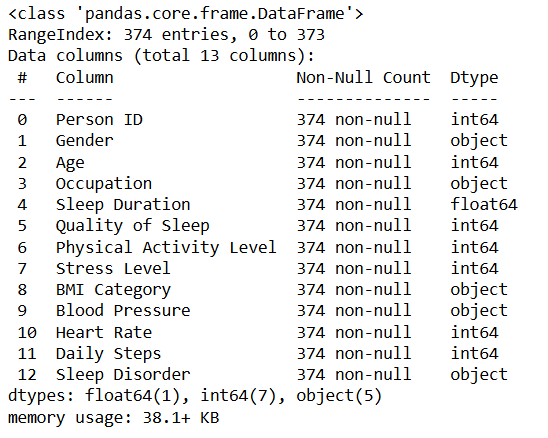
\includegraphics[width=0.75\linewidth]{img/df_info.png}
        \caption{Descripción de los tipos de datos de las variables del dataset.}
        \label{fig:df_info}
    \end{figure}
    
    \item \textbf{Valores nulos:} no se detectaron valores ausentes en ninguna columna (\texttt{df.isnull().sum()} devolvió cero en todos los casos), por lo que no fue necesario aplicar imputaciones.
    
    \item \textbf{Duplicados:} tampoco se encontraron registros duplicados (\texttt{df.duplicated().sum()} = 0), lo cual garantiza que cada fila representa a un individuo único.
    
    \item \textbf{Resumen estadístico:} el método \texttt{df.describe()} mostró que las variables numéricas presentaban rangos clínicamente válidos. Por ejemplo, la edad oscilaba entre 27 y 59 años, la frecuencia cardíaca entre 65 y 86 lpm, y la duración del sueño entre 5.8 y 8.5 horas.
    
    \begin{figure}[H]
        \centering
        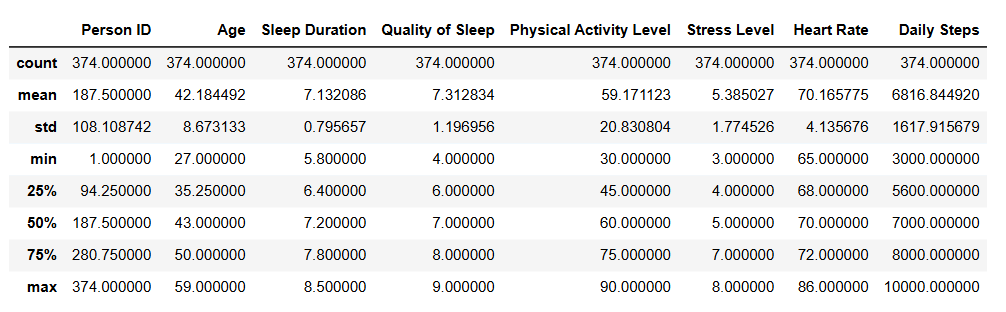
\includegraphics[width=0.9\linewidth]{img/df_describe.png}
        \caption{Resumen estadístico de las variables numéricas del dataset.}
        \label{fig:df_describe}
    \end{figure}
    
    \item \textbf{Variables categóricas:} se inspeccionaron los valores únicos de columnas como \texttt{Gender}, \texttt{Occupation} y \texttt{BMI Category}. Se identificaron dos categorías de género, once ocupaciones distintas y cuatro categorías de IMC (Índice de Masa Corporal). Se detectó una etiqueta duplicada en la variable \texttt{BMI Category} (“Normal Weight”), que se unificó con “Normal” para evitar ambigüedades durante la codificación.

    \begin{figure}[H]
        \centering
        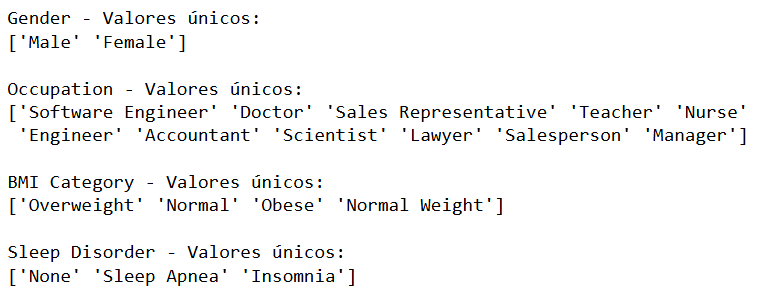
\includegraphics[width=0.8\linewidth]{img/columnasCategoricas.png}
        \caption{Descripción de los valores posibles en las variables categóricas.}
        \label{fig:columnas-categoricas}
    \end{figure}
    
\end{itemize}

\subsubsection{Eliminación de variables no predictivas}

Se eliminó la columna \texttt{Person ID}, ya que su única función era actuar como identificador único de registros. Al no aportar información útil para la predicción, se consideró una variable irrelevante desde el punto de vista del modelado.



\subsection{Análisis exploratorio de datos (EDA)}

El análisis exploratorio de datos (EDA, por sus siglas en inglés) constituye una etapa clave para comprender la estructura del conjunto de datos, identificar anomalías, explorar distribuciones y relaciones entre variables, y orientar las decisiones posteriores sobre preprocesamiento, selección de variables y diseño del modelo.


\subsubsection{Distribución de variables numéricas}

Para cada variable continua se generaron cuatro representaciones gráficas: \textbf{boxplot}, \textbf{violin plot}, \textbf{KDE plot} y \textbf{histograma}, con el objetivo de examinar su distribución, simetría y posibles valores atípicos desde distintos enfoques. A continuación, se muestran algunos ejemplos representativos.

\begin{figure}[H]
    \centering
    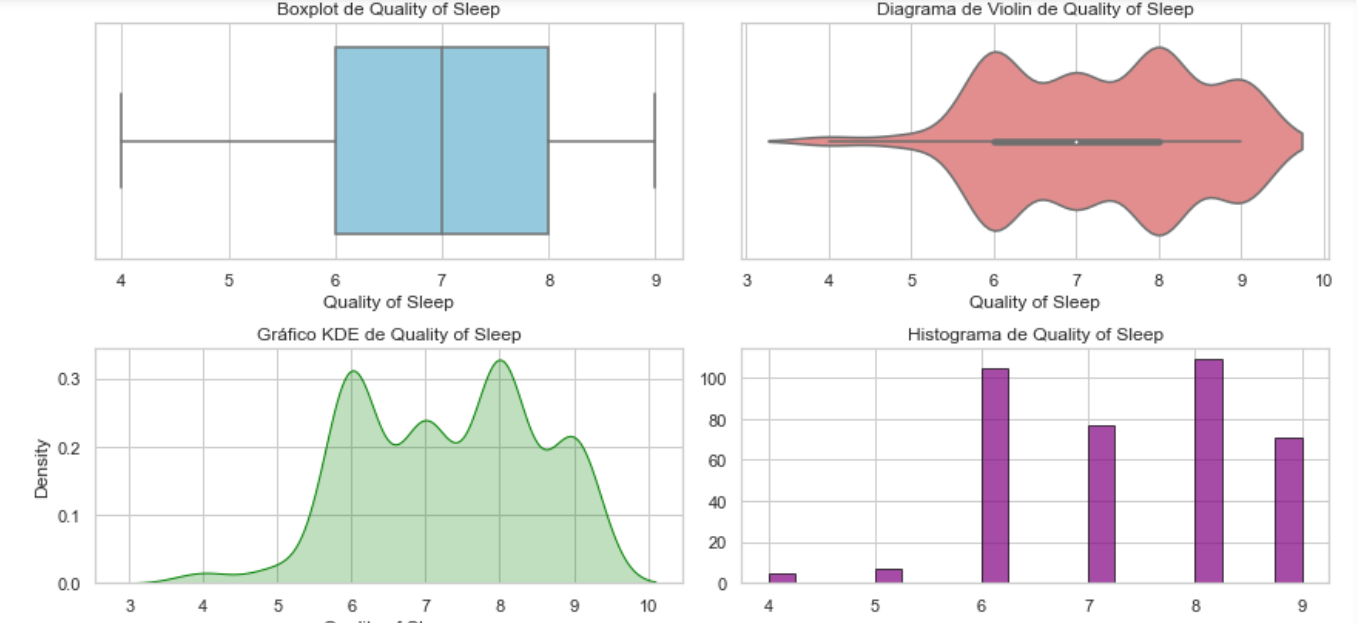
\includegraphics[width=1\linewidth]{img/qualitySleep.png}
    \caption{Distribución de la variable \textit{Quality of Sleep} mediante diferentes representaciones gráficas.}
\end{figure}

También se analizaron estas variables diferenciando por clase de trastorno del sueño, lo que permitió identificar patrones relevantes. Por ejemplo, se observó que los sujetos con insomnio tendían a concentrarse en valores bajos de duración del sueño.

\begin{figure}[H]
    \centering
    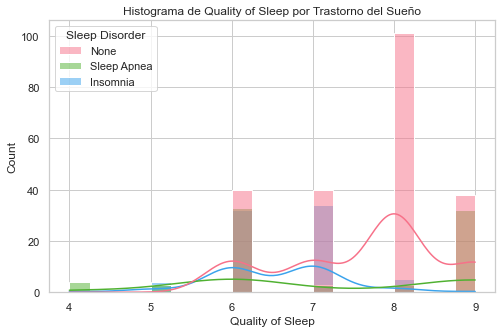
\includegraphics[width=1\linewidth]{img/qualityTrastorno.png}
    \caption{Distribución de la variable \textit{Quality of Sleep} por clase de trastorno del sueño mediante histograma con curva KDE.}
    \label{fig:hist_quality_sleep}
\end{figure}

\begin{figure}[H]
    \centering
    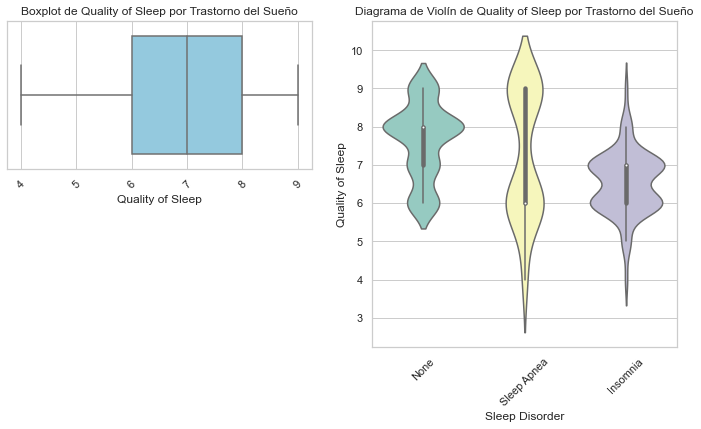
\includegraphics[width=1\linewidth]{img/qualityBoxTrastorno.png}
    \caption{Distribución de la variable \textit{Quality of Sleep} por clase de trastorno del sueño mediante boxplot y diagrama de violín.}
    \label{fig:box_violin_quality_sleep}
\end{figure}



\subsubsection{Distribución de variables categóricas}

Se exploraron visualmente las variables categóricas \texttt{Gender}, \texttt{Occupation}, \texttt{BMI Category} y \texttt{Sleep Disorder}. En la Figura~\ref{fig:ocupacion_clase}, se muestra la distribución de ocupaciones por clase.

\begin{figure}[H]
    \centering
    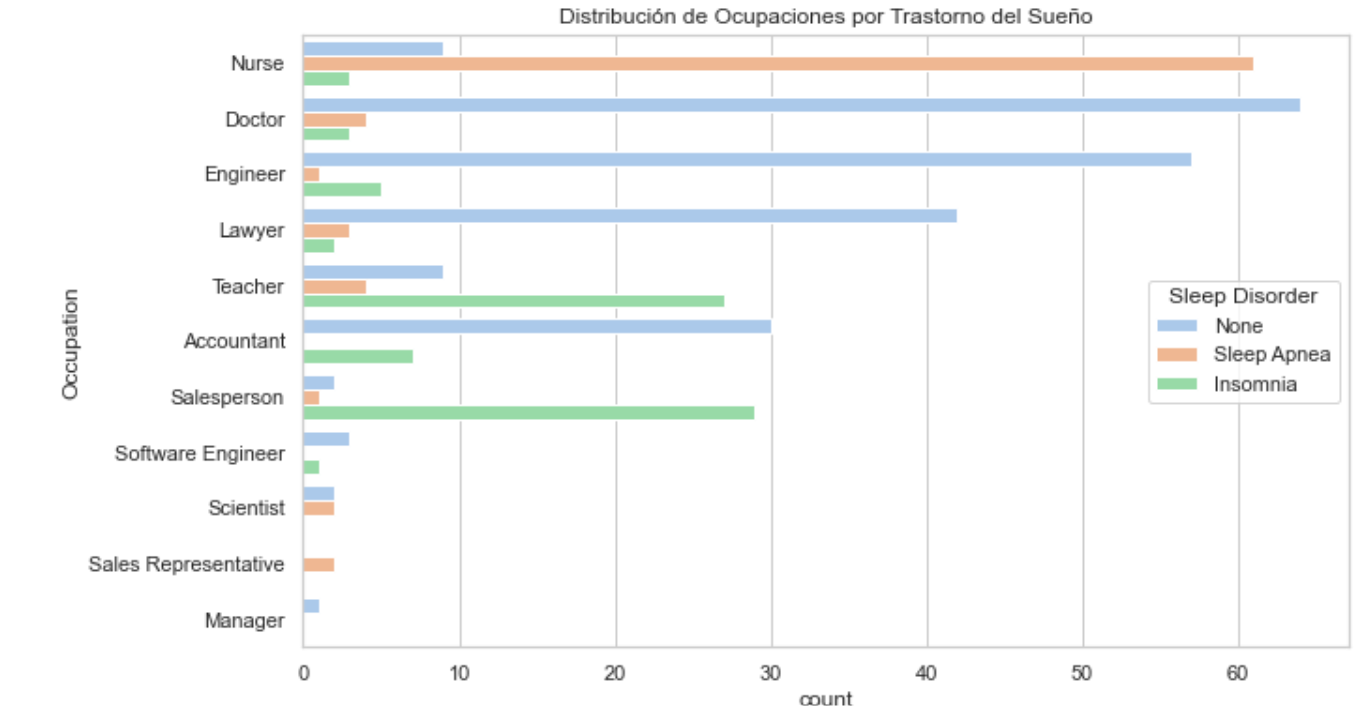
\includegraphics[width=1\linewidth]{img/ocupacionesClase.png}
    \caption{Distribución de la variable \texttt{Occupation} por clase.}
    \label{fig:ocupacion_clase}
\end{figure}

En la Figura~\ref{fig:bmi_trastorno} se muestra un ejemplo representativo, donde se observa que la categoría \textit{Normal} es predominante entre individuos sin trastorno, mientras que las categorías \textit{Overweight} y \textit{Obese} presentan mayor proporción de casos con apnea del sueño o insomnio.


\begin{figure}[H]
    \centering
    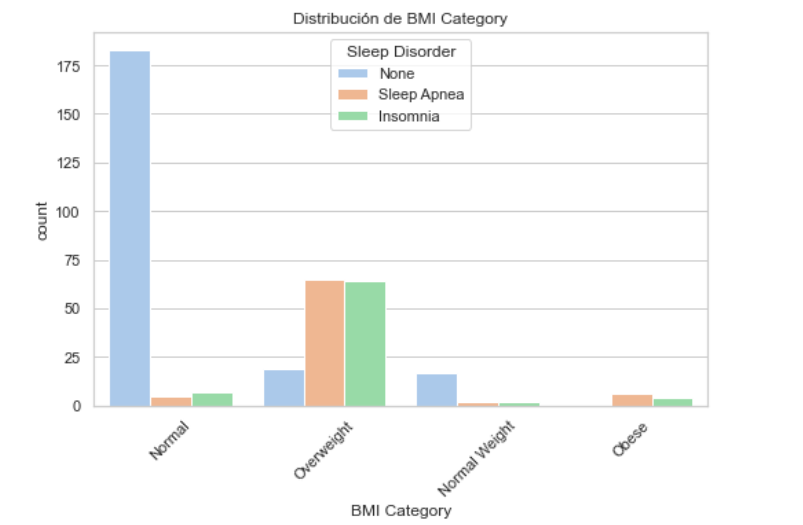
\includegraphics[width=1\linewidth]{img/IMCtrastorno.png}
    \caption{Distribución de categorías de IMC (\texttt{BMI Category}) según tipo de trastorno del sueño.}
    \label{fig:bmi_trastorno}
\end{figure}

Este análisis permitió observar que ciertas ocupaciones como \textit{Nurse} o \textit{Salesperson} estaban sobrerrepresentadas en casos de insomnio o apnea del sueño, lo que podría estar relacionado con patrones ocupacionales de riesgo, aportando una posible interpretación clínica.

\subsubsection{Detección de outliers}

Para complementar el análisis visual mediante diagramas de caja y violín, se aplicó un enfoque estadístico basado en el rango intercuartílico (IQR) con el objetivo de identificar valores atípicos de forma cuantitativa. Este método establece umbrales inferior y superior para cada variable numérica, definidos como:

\[
\text{IQR} = Q_3 - Q_1 \qquad 
\text{Límite inferior} = Q_1 - 1.5 \cdot \text{IQR} \qquad 
\text{Límite superior} = Q_3 + 1.5 \cdot \text{IQR}
\]

Se evaluaron las siguientes variables numéricas: edad, duración del sueño, calidad del sueño, nivel de estrés, pasos diarios, frecuencia cardíaca y nivel de actividad física. Como resultado, se identificaron un total de 15 registros con valores fuera de los límites definidos, todos ellos correspondientes a la variable \texttt{Heart Rate}.


\begin{table}[H]
    \centering
    \begin{tabular}{l|c}
        \textbf{Variable} & \textbf{Outliers detectados} \\
        \hline
        Heart Rate & 15 \\
        Todas las demás & 0
    \end{tabular}
    \caption{Número de outliers detectados por variable (método IQR).}
\end{table}

Estos registros no fueron eliminados del conjunto de datos, ya que se consideró que podrían representar condiciones clínicas reales, como bradicardia, que pueden ser relevantes para el diagnóstico de ciertos trastornos del sueño. Esta decisión se tomó en línea con el criterio clínico de conservar la heterogeneidad natural de la muestra.



\subsubsection{Correlaciones entre variables}

Se construyó un mapa de calor con el coeficiente de correlación de Pearson para identificar relaciones lineales entre variables numéricas. Destacó una fuerte correlación positiva entre presión sistólica y diastólica ($r \approx 0.97$), así como una correlación negativa entre calidad del sueño y nivel de estrés.

\begin{figure}[H]
    \centering
    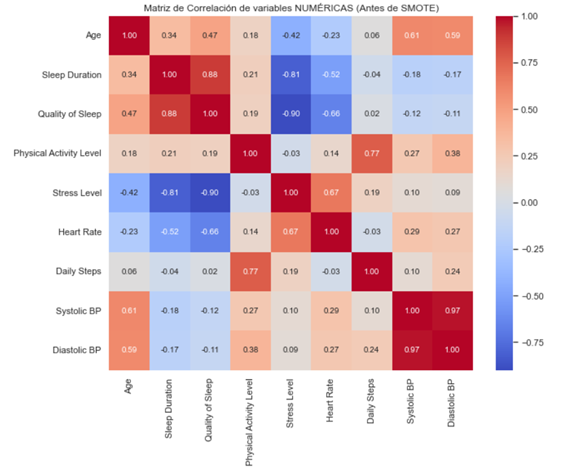
\includegraphics[width=1\linewidth]{img/heatmap.png}
    \caption{Mapa de correlaciones entre variables numéricas.}
    \label{fig:heatmap}
\end{figure}

\subsubsection{Distribución de la variable objetivo}

La variable objetivo \texttt{Sleep Disorder} incluye tres clases: \texttt{None}, \texttt{Insomnia} y \texttt{Sleep Apnea}. En la Figura~\ref{fig:dist_clases} se observa un claro desbalance: la clase \texttt{None} representa más del 50\% de los registros, mientras que las clases patológicas tienen una representación significativamente menor.

\begin{figure}[H]
    \centering
    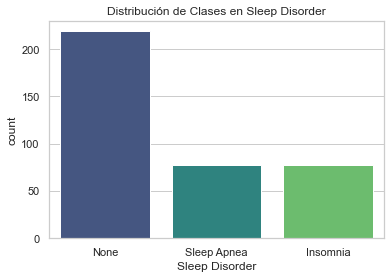
\includegraphics[width=0.75\linewidth]{img/countplot_SleepDisorders.png}
    \caption{Distribución de clases en la variable \textit{Sleep Disorder}.}
    \label{fig:dist_clases}
\end{figure}

Este desequilibrio fue tenido en cuenta durante la fase de modelado, donde se evaluaron técnicas de balanceo específicas que se describen más adelante.


\subsubsection{Importancia de características}

Como parte del análisis exploratorio, se evaluó la influencia relativa de cada variable sobre la predicción de los trastornos del sueño. Se aplicaron múltiples técnicas de selección de características, tanto basadas en modelos como en estadística:

\begin{itemize}
    \item \textbf{Random Forest:} se analizaron las reducciones de impureza en cada nodo para estimar la importancia de las variables. La Figura~\ref{fig:feature_rf} muestra el resultado de este análisis.
    \item \textbf{SelectKBest:} se utilizaron pruebas estadísticas como $\chi^2$ (para variables categóricas) y ANOVA-F (para numéricas) para valorar la relación con la variable objetivo.
    \item \textbf{RFE (Recursive Feature Elimination):} se entrenó un modelo de regresión logística que eliminaba iterativamente las variables menos relevantes hasta seleccionar las más influyentes.
\end{itemize}

\begin{figure}[H]
    \centering
    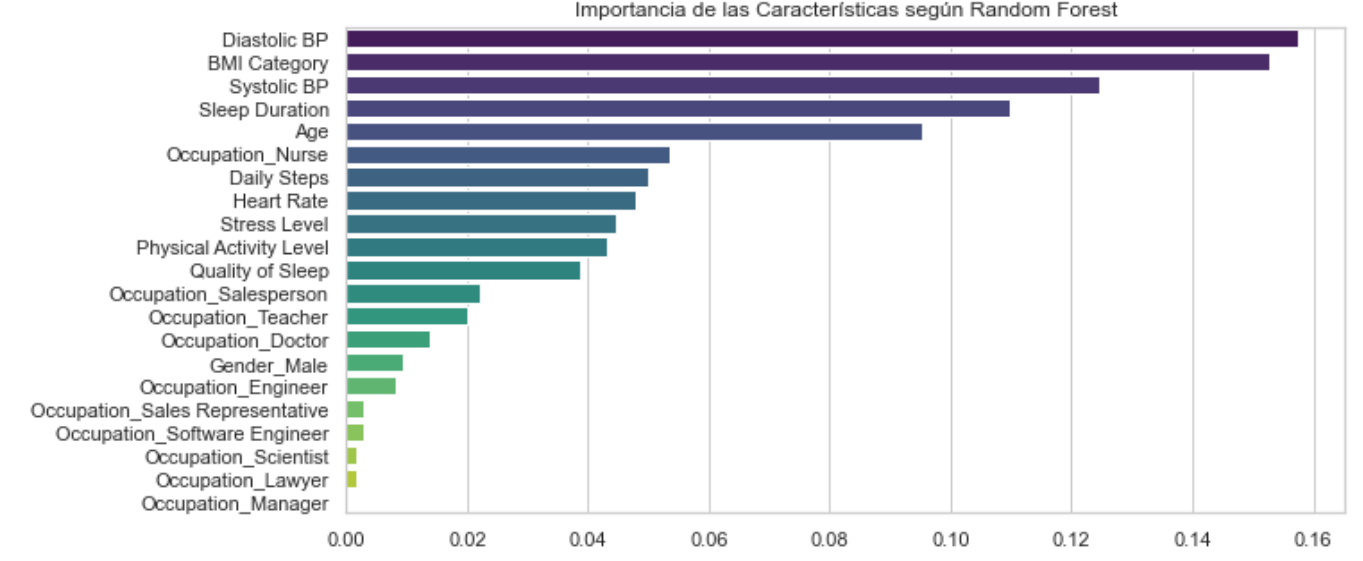
\includegraphics[width=1\linewidth]{img/importanciaRF.png}
    \caption{Importancia de características según Random Forest.}
    \label{fig:feature_rf}
\end{figure}

Las variables más destacadas por varias técnicas fueron: \textit{BMI Category}, \textit{Diastolic BP}, \textit{Occupation\_Nurse} y \textit{Sleep Duration}. No obstante, se optó por conservar todas las variables, priorizando la interpretabilidad y evitando eliminar características que podrían tener valor clínico no capturado por su peso estadístico.


El análisis exploratorio no solo permitió detectar posibles sesgos en la distribución de las clases y evaluar la calidad general del dataset, sino también orientar decisiones clave en el diseño del modelo, como la necesidad de calibración, la selección de variables relevantes y la elección de algoritmos robustos frente al desbalance de clases. 

Este análisis estableció así una base sólida para el posterior preprocesamiento de los datos, asegurando que las transformaciones aplicadas respondieran a patrones reales del conjunto y no a artefactos o desequilibrios ocultos.



\subsection{Preprocesamiento}

Una vez finalizado el análisis exploratorio, se procedió al preprocesamiento del conjunto de datos. Esta fase incluyó transformaciones esenciales para preparar las variables para su uso eficiente en modelos de aprendizaje automático, garantizando al mismo tiempo la coherencia clínica y semántica de la información.


\subsubsection{Codificación de variables categóricas}

Las variables categóricas se transformaron en variables numéricas utilizando dos enfoques diferenciados:

\begin{itemize}
    \item \textbf{One-Hot Encoding}, aplicado a variables nominales como \texttt{Gender} y \texttt{Occupation}, generando una columna binaria por cada categoría posible.
    \item \textbf{Label Encoding}, utilizado para la variable ordinal \texttt{BMI Category}, respetando su orden lógico clínico: \textit{Underweight < Normal < Overweight < Obese}.
\end{itemize}

El uso combinado de codificación binaria para variables nominales y ordinal para escalas clínicas asegura que la semántica original no se pierda durante el modelado. Tras la codificación, se conservaron todas las variables generadas, incluyendo las columnas binarias del \textit{one-hot encoding}, con el objetivo de mantener el máximo contexto clínico durante la predicción.

\subsubsection{Estandarización de variables numéricas}

Con el fin de homogeneizar la escala de las variables continuas y facilitar su procesamiento por parte de los algoritmos, se aplicaron técnicas de escalado a las siguientes variables:

\begin{itemize}
    \item Age
    \item Sleep Duration
    \item Quality of Sleep
    \item Physical Activity Level
    \item Stress Level
    \item Daily Steps
    \item Heart Rate
    \item Systolic BP
    \item Diastolic BP
\end{itemize}

Aunque inicialmente se evaluó el uso de \texttt{StandardScaler}, que transforma los datos a una distribución con media cero y desviación estándar uno, se observó que este método generaba valores negativos, lo cual dificultaba la representación visual en la aplicación interactiva y reducía su interpretabilidad para usuarios no técnicos. Por ello, se optó finalmente por \texttt{MinMaxScaler}, que transforma las variables al rango [0, 1], preservando la proporcionalidad relativa entre valores y facilitando su uso clínico y visual.


\subsubsection{División del conjunto de datos}

Finalmente, se realizó la partición del dataset en dos subconjuntos: un 80\% para entrenamiento y un 20\% para validación. Se utilizó la función \texttt{train\_test\_split} con la opción de \textbf{estratificación} sobre la variable \texttt{Sleep Disorder}, asegurando así que la distribución de clases se mantuviera proporcional en ambos subconjuntos. Esta estrategia es especialmente importante en tareas multiclase con clases desbalanceadas, como en este caso, donde la clase \texttt{None} es mayoritaria.

Tras completar estas transformaciones, el conjunto de datos quedó preparado para su uso en las fases de entrenamiento, validación cruzada y evaluación comparativa de modelos multiclase.


\begin{table}[H]
\centering
\begin{tabular}{ll}
\toprule
\textbf{Proceso} & \textbf{Descripción} \\
\midrule
Codificación      & One-Hot y Label Encoding \\
Escalado          & MinMaxScaler (rango [0, 1]) \\
Partición de datos & 80\% entrenamiento / 20\% test, con estratificación \\
\bottomrule
\end{tabular}
\caption{Resumen de las transformaciones aplicadas durante el preprocesamiento.}
\end{table}


\subsection{Desarrollo y selección de modelos predictivos}

Una vez completado el preprocesamiento, se procedió al entrenamiento de distintos modelos de clasificación multiclase con el objetivo de predecir si un individuo presenta insomnio, apnea del sueño o ausencia de trastornos. Para ello, se evaluaron cinco algoritmos clásicos de aprendizaje automático, implementados en la biblioteca \textit{scikit-learn}\footnote{\href{https://scikit-learn.org/}{Librería de scikit-learn.}}:

\begin{itemize}
    \item Regresión logística (\textit{Logistic Regression})
    \item Árboles de decisión (\textit{Decision Tree})
    \item Máquina de vectores soporte (\textit{SVM})
    \item Perceptrón multicapa (\textit{MLP})
    \item Bosques aleatorios (\textit{Random Forest})
\end{itemize}

La evaluación inicial se realizó mediante validación cruzada estratificada (\texttt{StratifiedKFold}) con cinco particiones (k=5). Como métrica principal se utilizó el \textbf{F1-score macro}, al ofrecer un mejor equilibrio entre clases desbalanceadas y evitar que la clase mayoritaria dominara el análisis global.

\subsubsection{Comparación inicial y efecto de SMOTE}

Dado el desequilibrio en la distribución de clases (mostrado en la Figura \ref{fig:dist_clases}) del conjunto de entrenamiento (\textit{None}: 175, \textit{Sleep Apnea}: 62, \textit{Insomnia}: 62), se evaluó la viabilidad de aplicar la técnica de sobremuestreo \textbf{SMOTE} (Synthetic Minority Oversampling Technique). Esta técnica genera ejemplos sintéticos de las clases minoritarias a partir de combinaciones lineales de muestras reales y sus vecinos más cercanos.

SMOTE se aplicó exclusivamente sobre el conjunto de entrenamiento, evitando así fugas de información. La distribución equilibrada resultante se muestra en la Figura~\ref{fig:distribucion_smote}.


\begin{figure}[H]
    \centering
    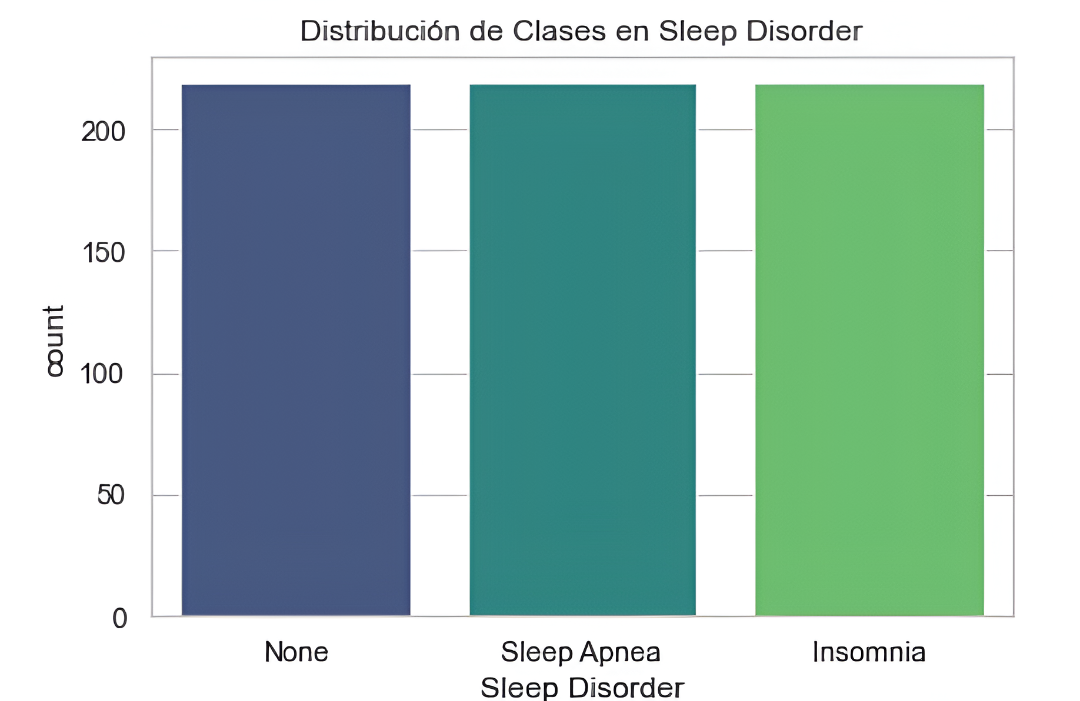
\includegraphics[width=0.75\linewidth]{img/sleepDesorder_smote.png}
    \caption{Distribución de clases tras aplicar SMOTE en el conjunto de entrenamiento.}
    \label{fig:distribucion_smote}
\end{figure}

Los resultados obtenidos con esta técnica se presentan y analizan en el capítulo de \ref{cap:resultados} Resultados.


\subsubsection{Ajuste de hiperparámetros}

Para cada modelo se llevó a cabo una fase de ajuste de hiperparámetros utilizando \texttt{RandomizedSearchCV} o \texttt{GridSearchCV}, en función del espacio de búsqueda y la complejidad computacional. En todos los casos se aplicó validación cruzada estratificada (k=5) sobre el conjunto de entrenamiento y se seleccionó el estimador que maximizaba el F1-score macro.

Los hiperparámetros explorados fueron:

\begin{itemize}
    \item \textbf{Random Forest:} \verb|n_estimators|, \verb|max_depth|, \verb|min_samples_split|, \verb|min_samples_leaf|, \verb|bootstrap|.
    \item \textbf{MLP:} \verb|hidden_layer_sizes|, \verb|activation|, \verb|solver|, \verb|alpha|, \verb|learning_rate|.
    \item \textbf{Regresión Logística:} \verb|penalty|, \verb|C|, \verb|solver|.
    \item \textbf{Decision Tree:} \verb|max_depth|, \verb|min_samples_leaf|, \verb|min_samples_split|, \verb|criterion|.
    \item \textbf{SVM:} \verb|C|, \verb|kernel|, \verb|gamma|.
\end{itemize}

Cada modelo óptimo fue almacenado para su posterior calibración, evaluación comparativa y posible integración en la aplicación web.

%%%% conceptos teoricos 3.6
\subsubsection{Criterios de evaluación clínica del modelo}

En el presente trabajo se abordó un problema de clasificación multiclase, cuyo objetivo era asignar a cada individuo una de tres clases posibles: \textit{None}, \textit{Insomnia} o \textit{Sleep Apnea}. La naturaleza desbalanceada de estas clases, así como la relevancia clínica de los falsos negativos y falsos positivos, exigió una evaluación más detallada que la mera tasa de aciertos.

\textbf{Matriz de confusión}\\

La matriz de confusión permite comparar las predicciones del modelo con las etiquetas reales, descomponiendo el rendimiento en los siguientes componentes:

\begin{itemize}
    \item \textbf{True Positives (TP)}: casos positivos correctamente clasificados.
    \item \textbf{True Negatives (TN)}: casos negativos correctamente clasificados.
    \item \textbf{False Positives (FP)}: casos negativos clasificados erróneamente como positivos.
    \item \textbf{False Negatives (FN)}: casos positivos que el modelo no ha detectado.
\end{itemize}

\textbf{Métricas derivadas}\\

A partir de esta matriz se calcularon las siguientes métricas:

\begin{itemize}
    \item \textbf{Accuracy} (exactitud): proporción total de aciertos del modelo.
    \begin{equation}
        \text { Accuracy }=\frac{TP+TN}{TP+TN+FP+FN}
    \end{equation}
    Aunque es una métrica útil como referencia general, puede ser engañosa en conjuntos desbalanceados.

    \item \textbf{Precision}: porcentaje de predicciones positivas que realmente lo son.
    \begin{equation}
        \text { Precision }=\frac{TP}{TP+FP}
    \end{equation}
    Esta métrica ayuda a controlar los falsos positivos, clave en contextos clínicos sensibles.

    \item \textbf{Recall} (sensibilidad):
    \begin{equation}
        \text { Recall }=\frac{TP}{TP + FN}
    \end{equation}
    Es crítica cuando el objetivo es no dejar casos sin detectar, como en el diagnóstico de apnea o insomnio.

    \item \textbf{F1-score}:
    \begin{equation}
        F1 = 2 \cdot \frac{\text { Precision } \cdot \text { Recall }}  {\text { Precision }+ \text { Recall }}
    \end{equation}
    Se trata de la media armónica entre precisión y recall, recomendada en contextos con clases poco representadas.

\end{itemize}

En este trabajo se utilizó el \textbf{F1-score macro}, que calcula el F1-score de cada clase por separado y luego hace la media no ponderada. Esto evita que la clase mayoritaria domine el análisis.

\textbf{Evaluación gráfica}\\

Para complementar las métricas numéricas, se utilizaron dos representaciones gráficas adicionales:

\begin{itemize}
    \item \textbf{Curva ROC-AUC (Receiver Operating Characteristic)}: muestra la relación entre la tasa de verdaderos positivos (TP) y la tasa de falsos positivos (FP) para distintos umbrales de decisión. El área bajo esta curva (AUC) resume la capacidad discriminativa del modelo:
    \begin{itemize}
        \item AUC = 0.5: rendimiento equivalente al azar.
        \item AUC = 1.0: modelo perfecto.
    \end{itemize}

    \item \textbf{Curva Precision-Recall (PR)}: especialmente útil en contextos clínicos desbalanceados. Representa el compromiso entre precisión y recall a diferentes umbrales, proporcionando una visión más realista de la eficacia del modelo en las clases minoritarias.
\end{itemize}

El uso conjunto de estas métricas permitió evaluar de manera robusta la calidad del modelo tanto a nivel global como por clase. Los valores obtenidos y sus implicaciones se analizan en el capítulo de \textbf{Resultados} (\ref{cap:resultados}) \cite{powers2020evaluation}.


\subsubsection{Análisis de la influencia de la variable \texttt{Occupation}}

Durante el análisis exploratorio se detectó que la variable \texttt{Occupation}, codificada mediante \textit{One-Hot Encoding}, mostraba asociaciones notables con las clases patológicas, especialmente con insomnio y apnea del sueño. Esta observación planteó la hipótesis de que el modelo pudier estar capturando patrones no generalizables derivados del pequeño tamaño del conjunto de datos o de correlaciones espurias.

Con el fin de valorar el impacto específico de esta variable, se desarrolló una versión alternativa del pipeline completo de entrenamiento en la que \texttt{Occupation} fue excluida antes del preprocesamiento. En esta variante se mantuvieron todas las transformaciones, técnicas de escalado, divisiones de datos y procedimientos de ajuste de hiperparámetros empleados en el modelo principal, de modo que la única diferencia fuera la presencia o ausencia de dicha variable.

Esta experimentación permitió establecer una base comparativa para evaluar en qué medida la variable ocupacional contribuía al rendimiento y comportamiento del sistema predictivo. Los resultados derivados de esta comparación se presentan y analizan en detalle en el capítulo~\ref{cap:resultados}.


\subsection{Interpretabilidad del modelo}

La interpretabilidad es especialmente relevante en el ámbito clínico, donde cada predicción automatizada puede influir en la toma de decisiones sobre la salud de una persona. Por ello, además de seleccionar el modelo \textit{Random Forest} como predeterminado por su rendimiento, se evaluó también su capacidad explicativa mediante técnicas de inteligencia artificial explicable.

El análisis de interpretabilidad se integró como parte del sistema para reforzar la confianza del usuario y garantizar que las decisiones del modelo puedan ser comprendidas tanto por profesionales como por pacientes.

\subsubsection{Importancia global de las variables}

Se generó un \textit{summary plot} (gráfico resumen) utilizando SHAP (\textit{SHapley Additive exPlanations}) para identificar las variables con mayor influencia en el conjunto de predicciones. Las características más relevantes fueron:

\begin{itemize}
    \item Presión arterial sistólica y diastólica
    \item Índice de masa corporal (BMI)
    \item Frecuencia cardíaca
    \item Duración del sueño
\end{itemize}

Las variables identificadas como más relevantes por SHAP coinciden con factores de riesgo ampliamente documentados en la literatura clínica, lo que refuerza la coherencia del modelo y su aceptación clínica.

\begin{figure}[H]
    \centering
    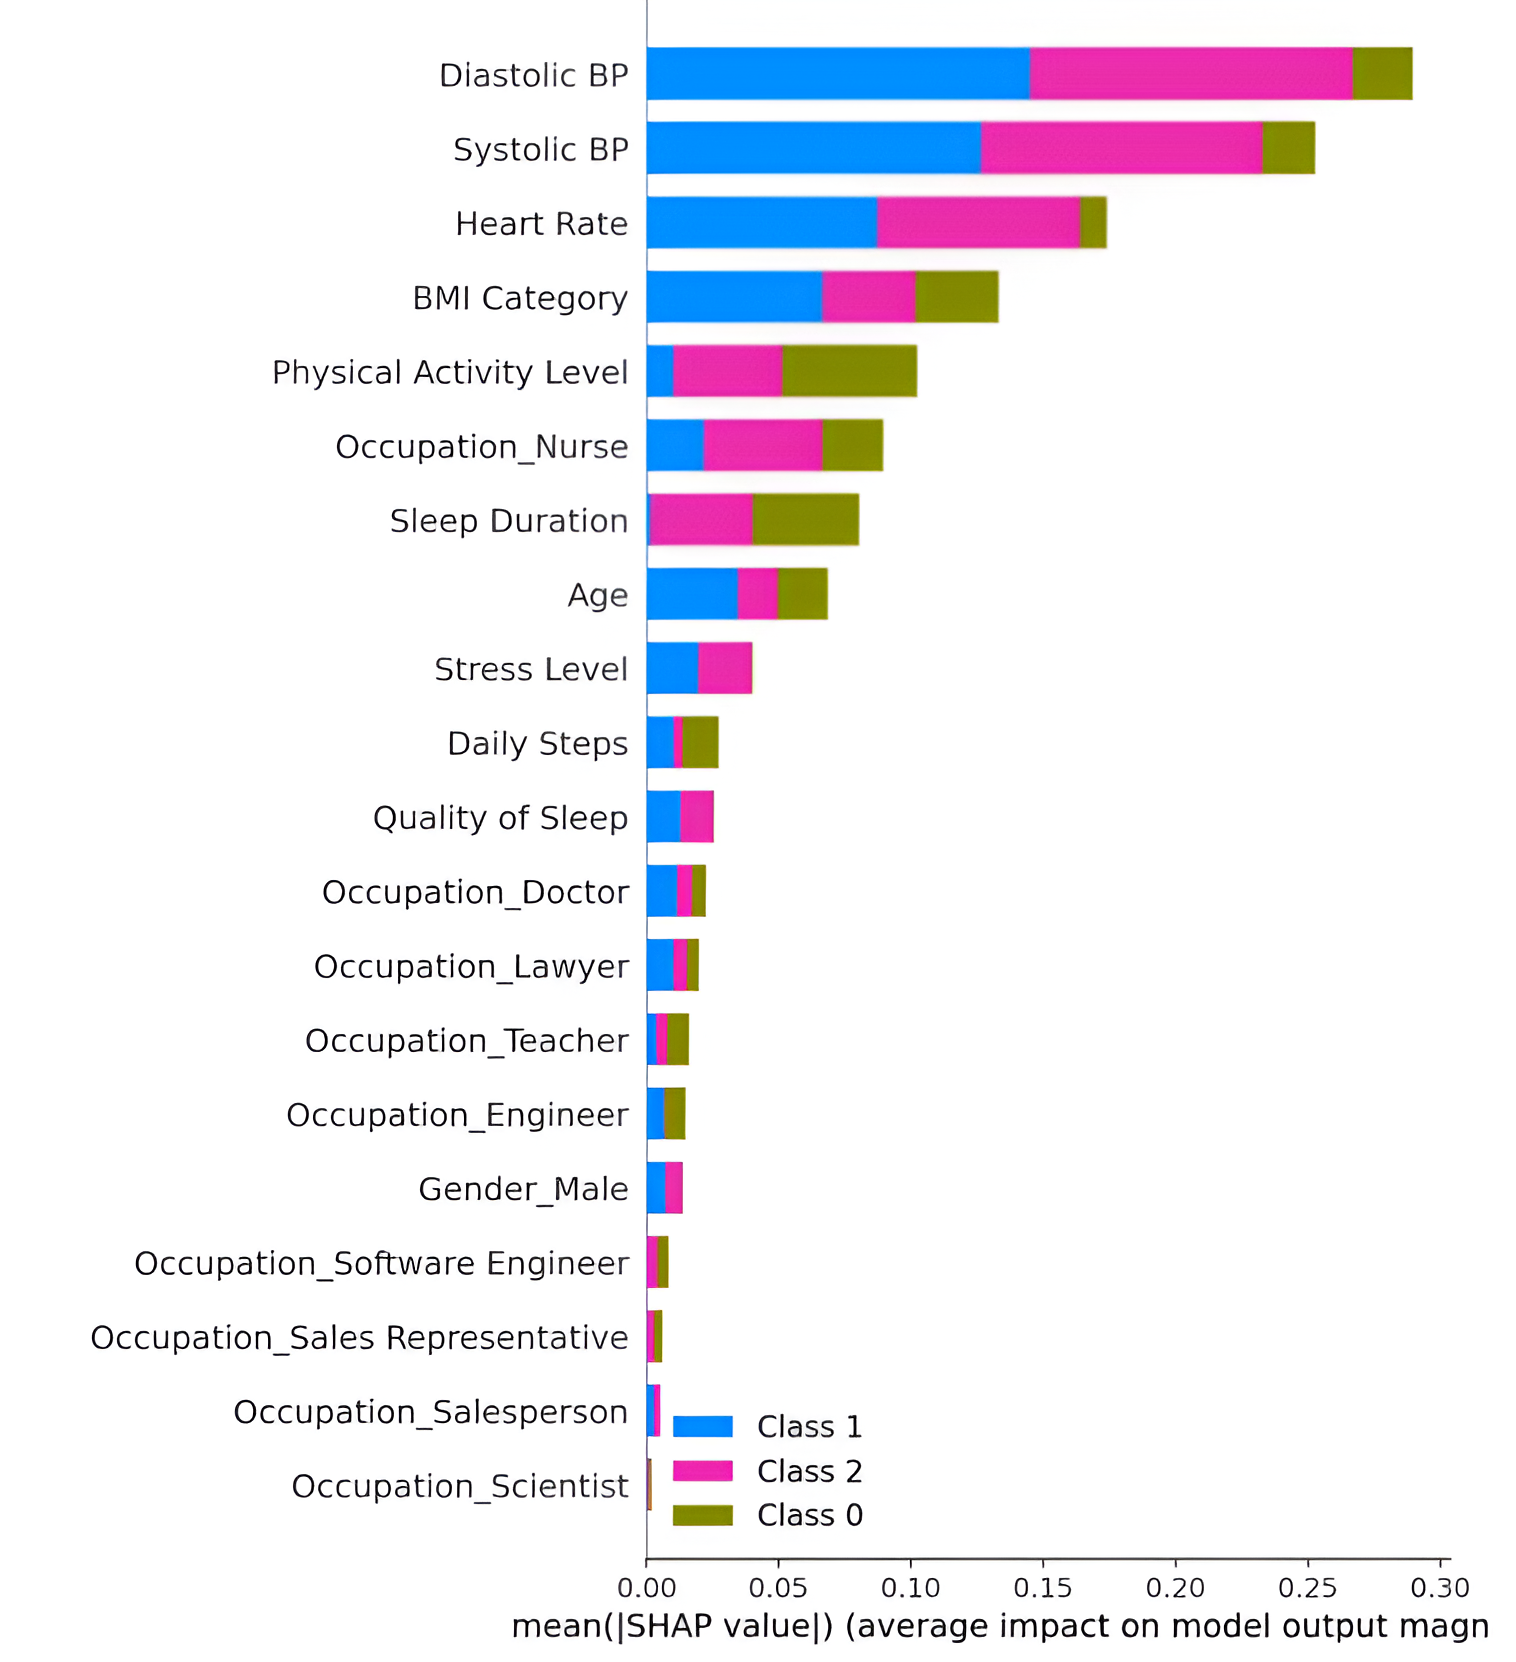
\includegraphics[width=0.85\linewidth]{img/SHAP.png}
    \caption{Gráfico resumen de SHAP: importancia media de cada variable}
    \label{fig:shap_summary}
\end{figure}

\subsubsection{Explicación individual de predicciones}
Para facilitar la interpretación de predicciones individuales, se utilizaron \textit{force plots} de SHAP. Estos gráficos descomponen la predicción mostrando cómo cada variable empuja la probabilidad hacia una clase concreta.

\begin{figure}[H]
    \centering
    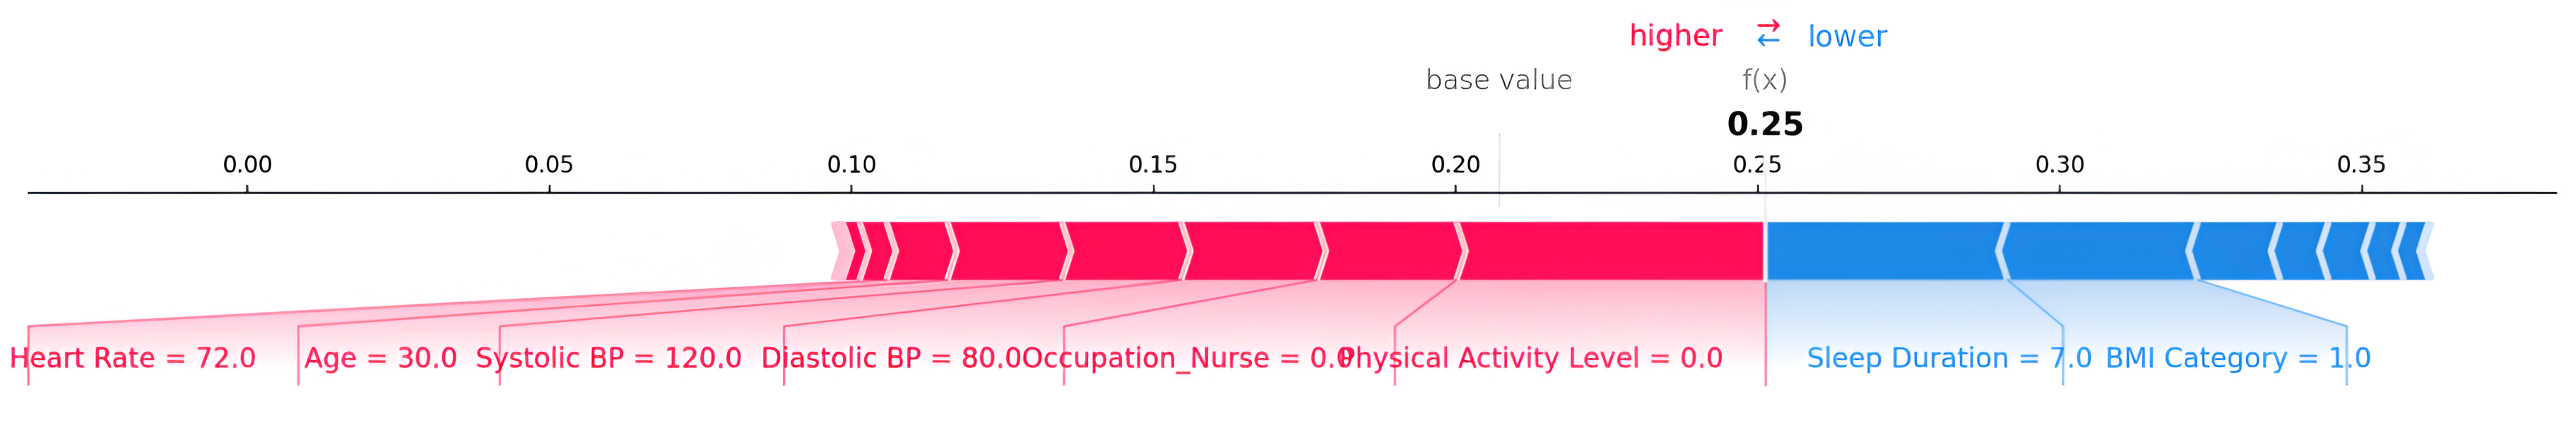
\includegraphics[width=1\linewidth]{img/explicacIndividual.png}
    \caption{Ejemplo de force plot para un individuo concreto}
    \label{fig:shap_force}
\end{figure}

Este enfoque mejora la transparencia del sistema y refuerza su utilidad en contextos donde se requiere trazabilidad de las decisiones.

\section{Implementación de la aplicación}

Con el objetivo de acercar el modelo predictivo al usuario final y facilitar su uso en contextos reales, se desarrolló una aplicación web interactiva mediante la librería \texttt{Streamlit}. Esta herramienta permitió construir una interfaz funcional directamente desde scripts de Python, sin necesidad de conocimientos en tecnologías web como HTML o JavaScript. El resultado fue una aplicación funcional, ligera y accesible desde cualquier dispositivo con conexión a internet.

\subsection{Objetivo y funcionalidades principales}

La aplicación permite introducir características personales y clínicas, realizar una predicción automática sobre el tipo de trastorno del sueño (o su ausencia), visualizar explicaciones basadas en SHAP y generar un informe en formato PDF.

El flujo de funcionamiento se estructura en las siguientes etapas:

\begin{enumerate}
    \item \textbf{Entrada de datos:} el usuario completa un formulario organizado en bloques, incluyendo edad, género, ocupación, calidad del sueño, presión arterial, IMC, nivel de estrés, pasos diarios, etc.
    \item \textbf{Preprocesamiento automático:} los datos son transformados mediante los mismos pasos aplicados en el entrenamiento (normalización y codificación One-Hot).
    \item \textbf{Predicción:} el modelo realiza la clasificación y devuelve las probabilidades asociadas a cada clase.
    \item \textbf{Visualización del resultado:} se muestra de forma clara la clase más probable junto con la probabilidad porcentual de cada una.
    \item \textbf{Explicabilidad:} se generan dos tipos de gráficos de SHAP: uno individual, que muestra qué variables influyeron más en la predicción concreta del usuario, y otro resumen global, que representa la importancia promedio de cada variable en el conjunto de datos.
    \item \textbf{Generación de informe:} se crea automáticamente un archivo PDF resumen con los datos introducidos, la predicción y la explicación visual.
\end{enumerate}

\subsection{Diseño y usabilidad}

La interfaz fue diseñada con criterios de claridad y usabilidad. Se utilizaron componentes interactivos como deslizadores, listas desplegables y botones de selección para facilitar la entrada de datos. El formulario está estructurado en dos columnas para una mejor experiencia visual, y los resultados se presentan con métricas porcentuales.

Además, se integraron funcionalidades adicionales como:

\begin{itemize}
    \item \textbf{Código QR dinámico:} insertado en la barra lateral para facilitar el acceso desde dispositivos móviles.
    \item \textbf{Generación automática de informes PDF:} utilizando la librería \texttt{FPDF}, con diseño clínico e información personalizada.
    \item \textbf{Gráficos SHAP:} tanto a nivel global (importancia de variables) como individual (force plot por paciente).
\end{itemize}

\subsection{Despliegue y validación}

La aplicación fue desplegada en la nube mediante \textbf{Streamlit Community Cloud}, lo que garantiza su accesibilidad sin necesidad de instalación local.

Para comprobar su correcto funcionamiento técnico, se realizaron pruebas de uso con distintos perfiles de entrada, simulando casos representativos de cada clase objetivo: sujetos sanos, con insomnio y con apnea del sueño. Estas pruebas permitieron validar el correcto flujo de datos desde el formulario hasta la generación de resultados e informes.

Adicionalmente, se contrastaron algunos perfiles simulados con informes reales obtenidos mediante el dispositivo O2Ring, durante una fase preliminar de desarrollo. Aunque no se realizó una integración directa con el dispositivo, esta comparación cualitativa permitió verificar la coherencia clínica del sistema y reforzar su aplicabilidad como herramienta complementaria de cribado o sensibilización.


\begin{figure}[H]
    \centering
    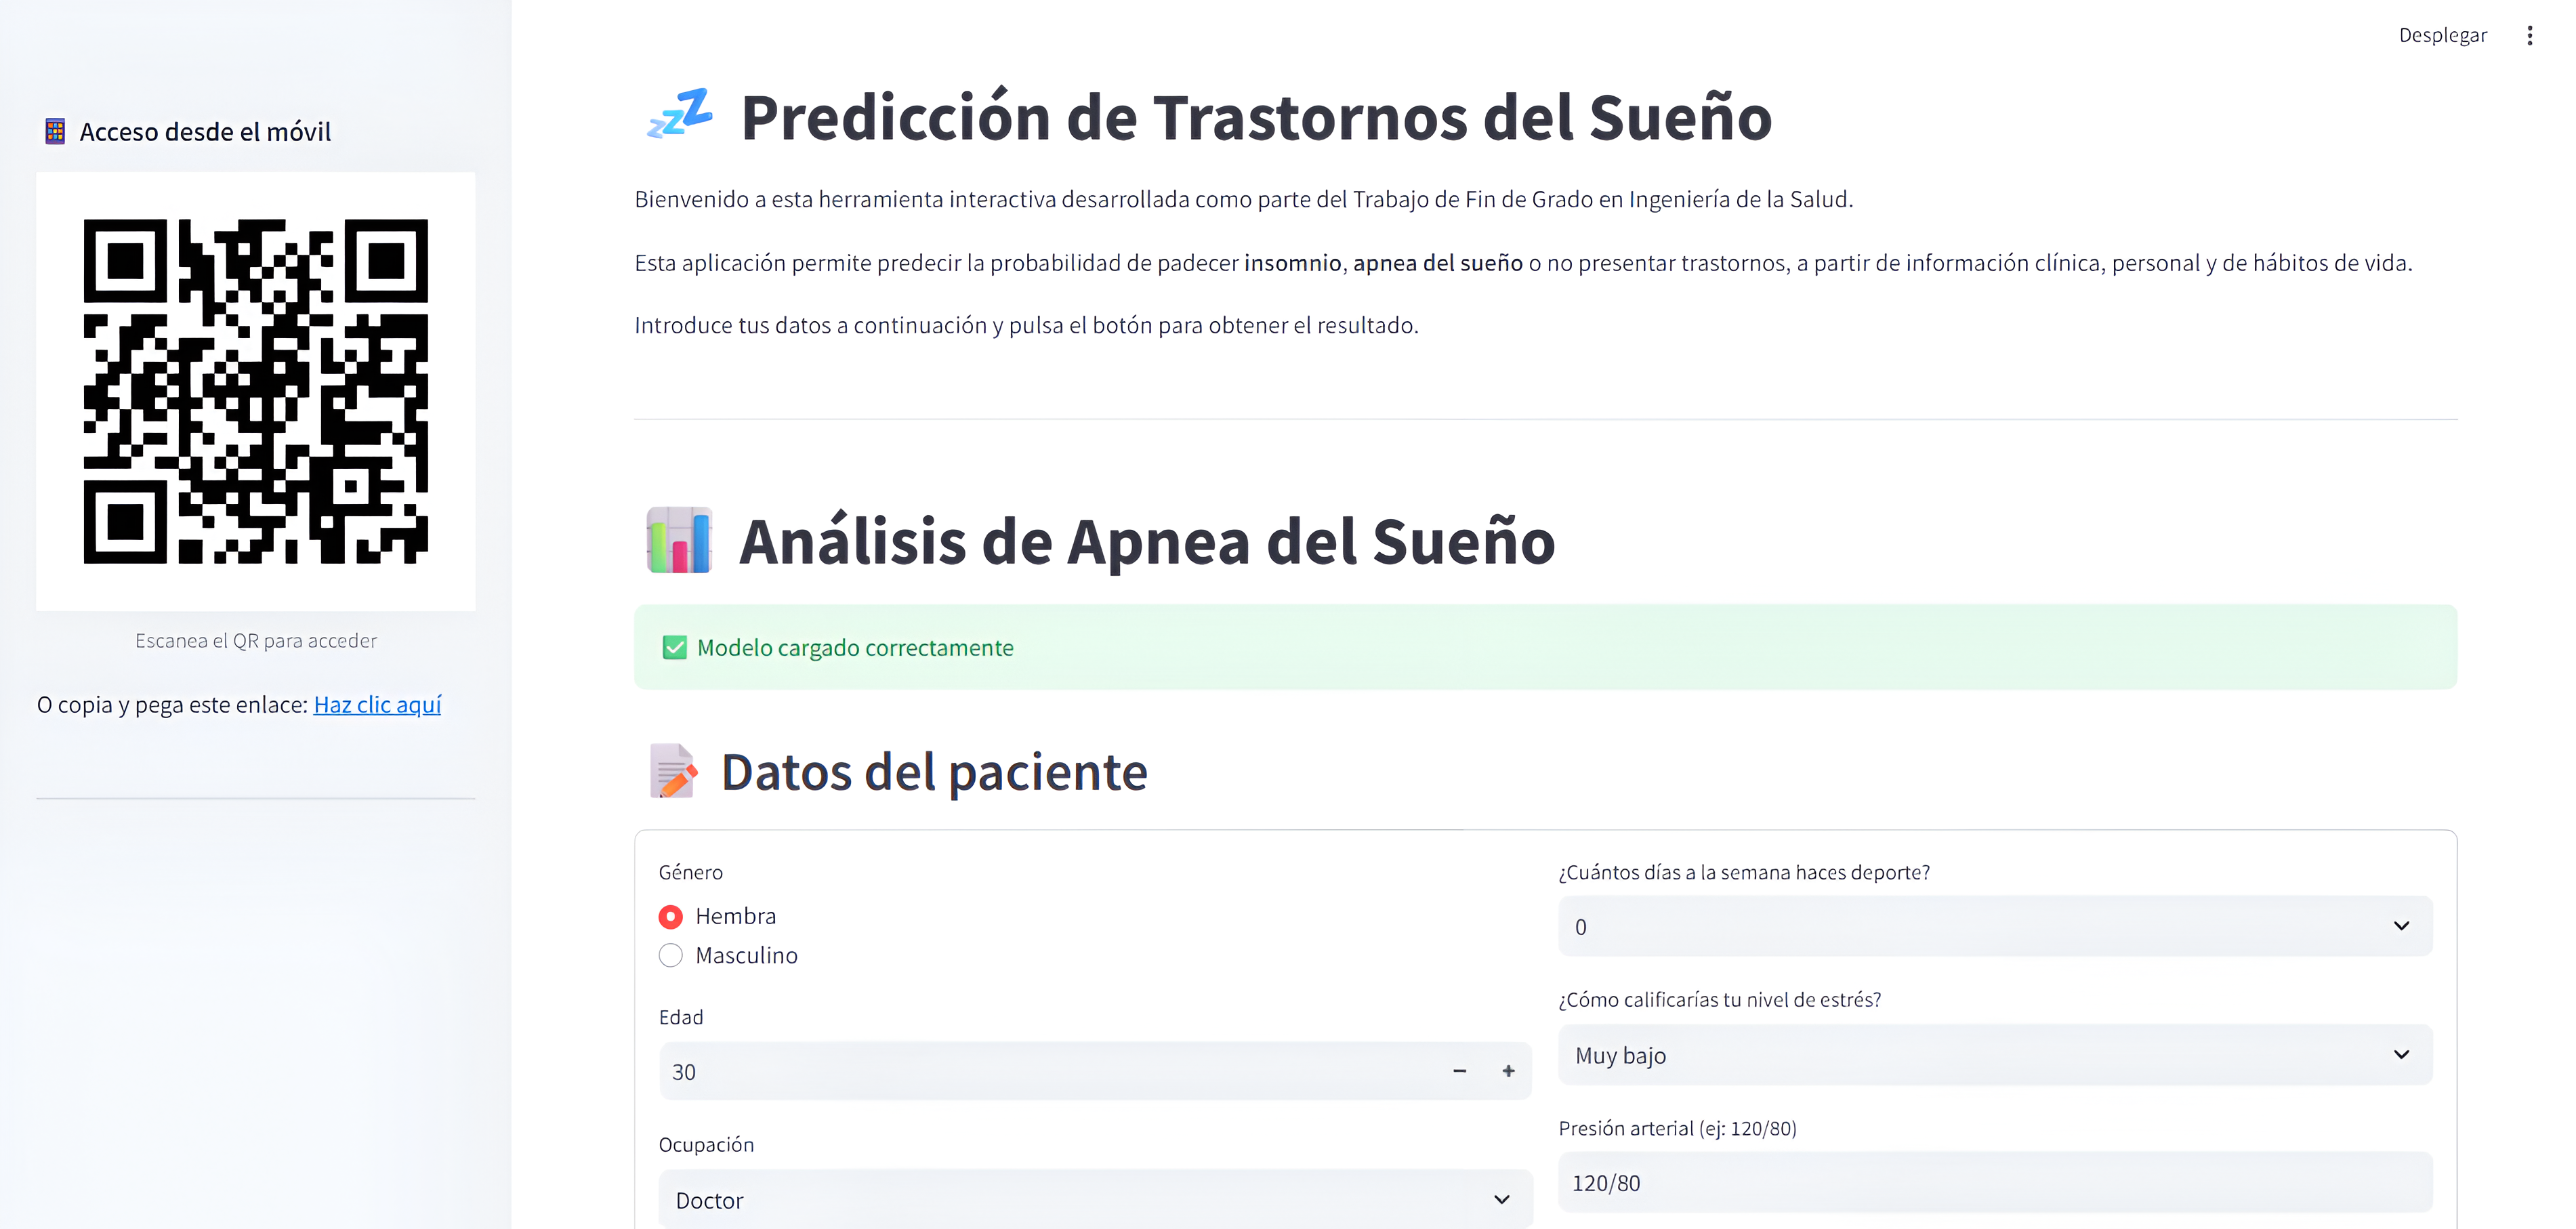
\includegraphics[width=1\linewidth]{img/interfazApp.png}
    \caption{Captura de la interfaz de la aplicación desarrollada en Streamlit.}
\end{figure}

\begin{figure}[H]
    \centering
    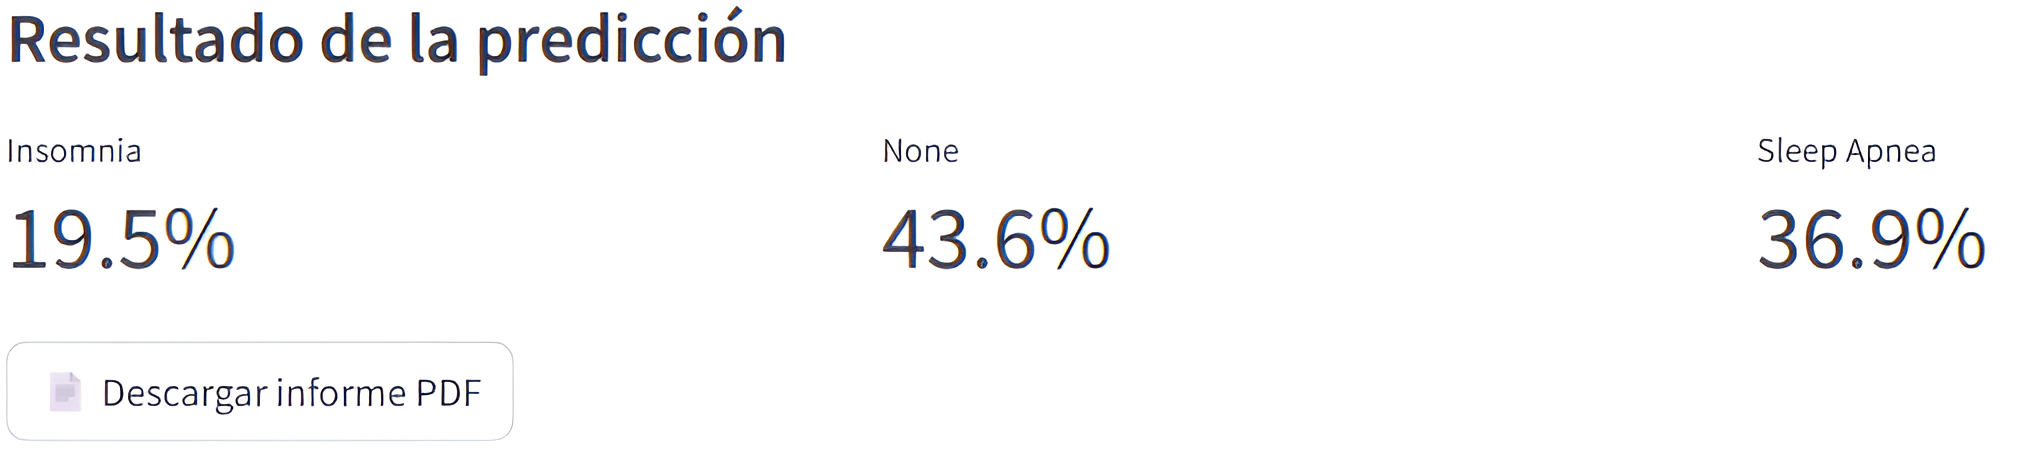
\includegraphics[width=0.9\textwidth]{img/resultadoPredd.png}
    \caption{Visualización de predicción.}
\end{figure}

\begin{figure}[H]
    \centering
    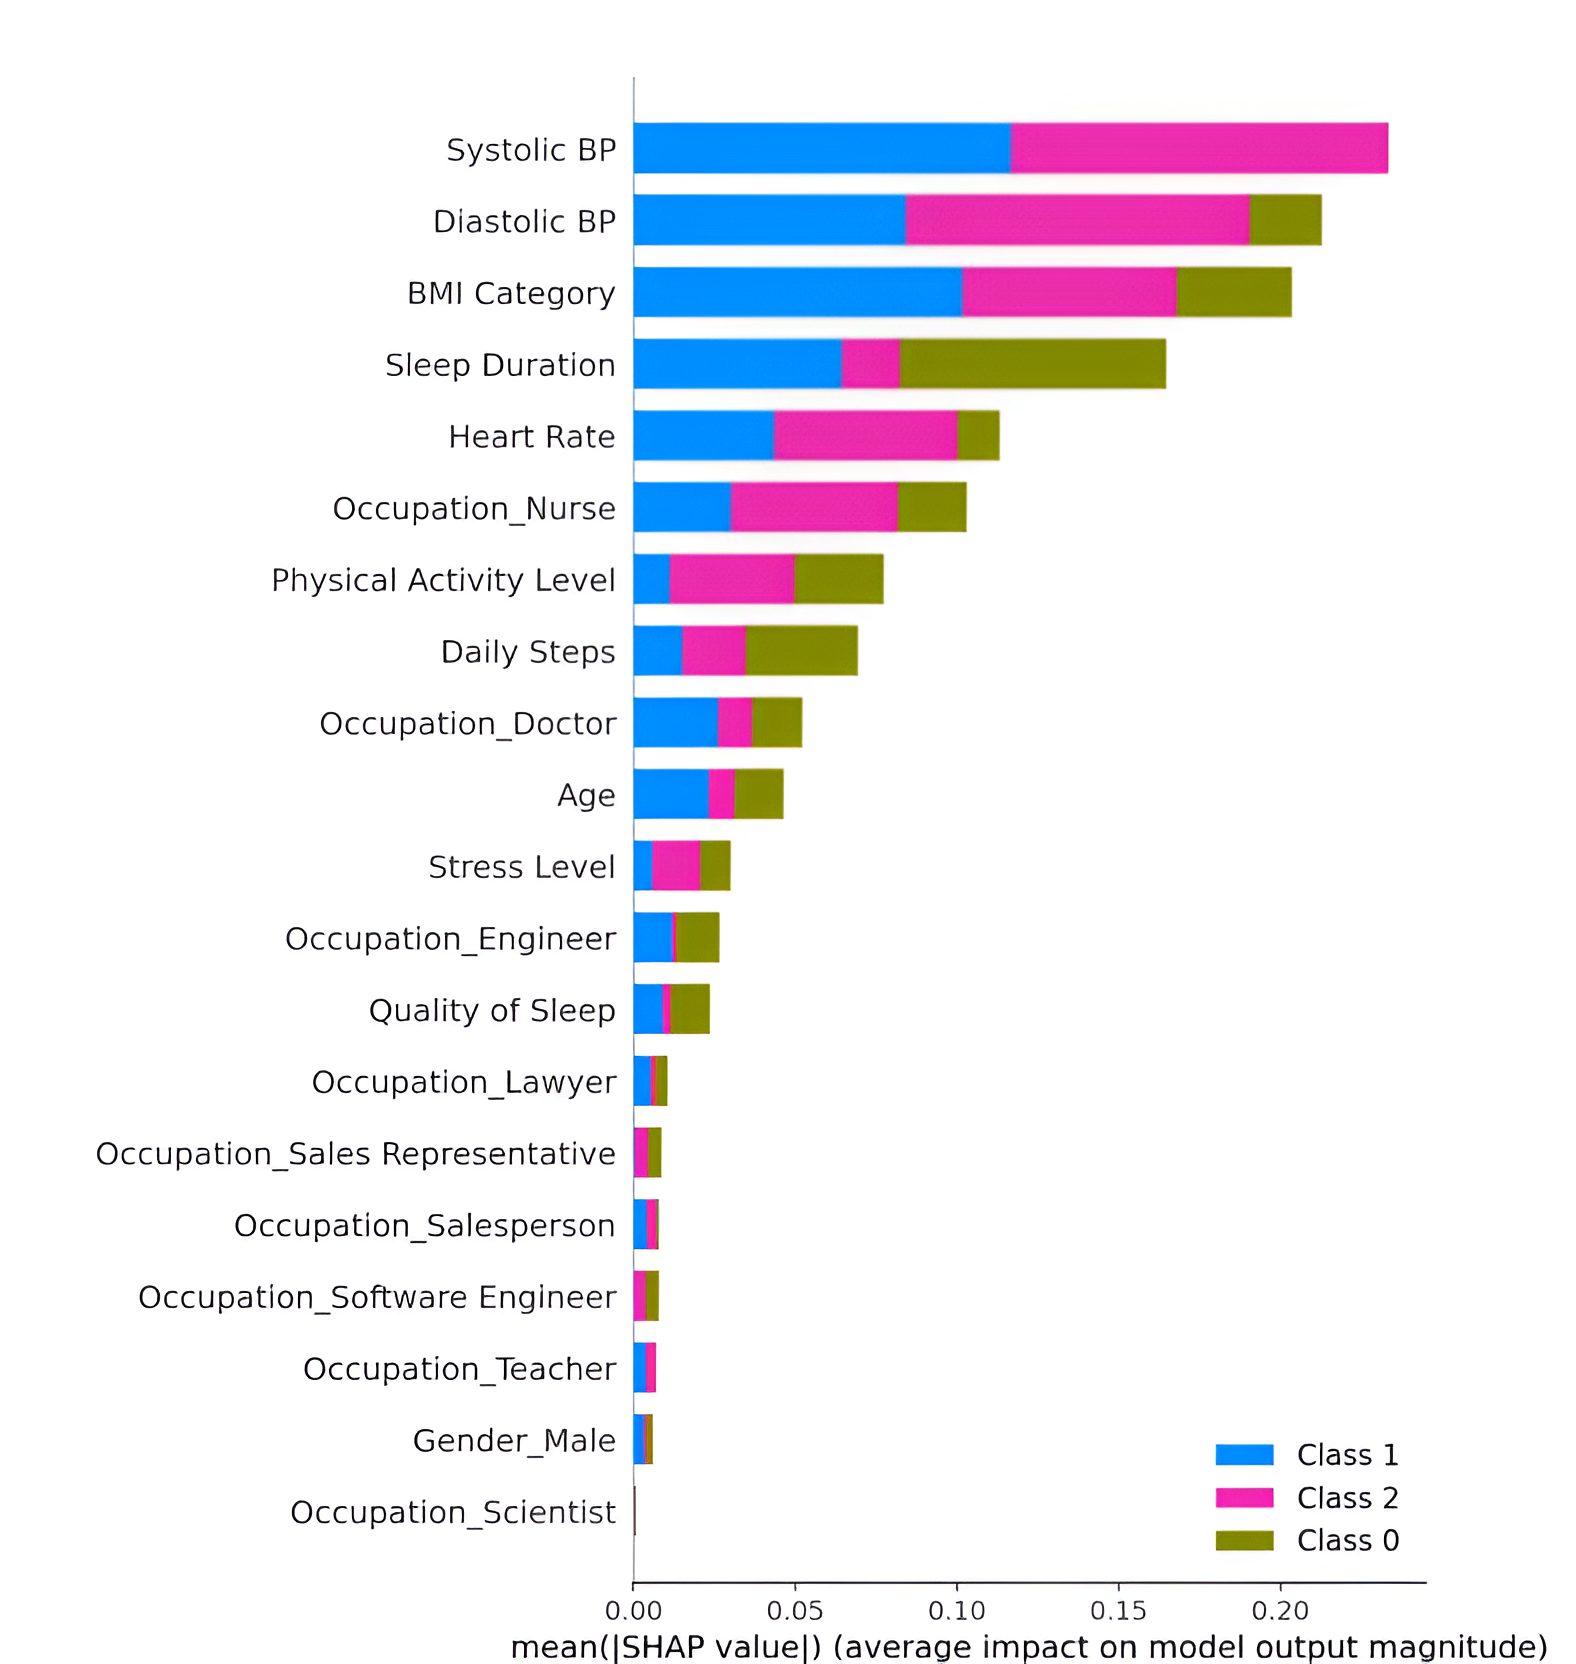
\includegraphics[width=0.75\linewidth]{img/shapApp.png}
    \caption{Explicación SHAP global en la interfaz.}
    \label{fig:shap}
\end{figure}


\begin{figure}[H]
    \centering
    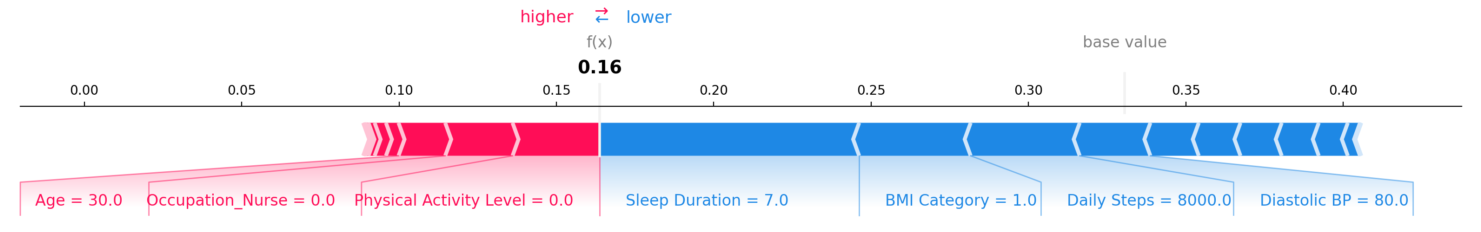
\includegraphics[width=1\linewidth]{img/explic_individual.png}
    \caption{Explicación SHAP individual.}
    \label{fig:shap}
\end{figure}


\section{Diseño de perfiles clínicos y validación externa}

Además de evaluar el rendimiento cuantitativo mediante métricas y representaciones gráficas, se consideró fundamental validar el sistema de forma práctica en situaciones clínicas. Para ello, se seleccionaron tres personas con características representativas de los tres grupos contemplados en la variable objetivo: pacientes con insomnio, con apnea del sueño y sin trastornos del sueño.

Estas personas fueron escogidas manualmente siguiendo criterios clínicos extraídos de la literatura científica y guías médicas sobre los principales factores de riesgo asociados a cada trastorno del sueño. A cada una se le colocó el dispositivo O2Ring para registrar sus variables fisiológicas reales, las cuales fueron posteriormente introducidas en la aplicación para comprobar la respuesta del modelo ante perfiles clínicamente relevantes.


\begin{itemize}
    \item \textbf{Factores de riesgo para Insomnio:} nivel de estrés elevado, mala calidad del sueño, duración inferior a 6 horas, baja actividad física, consumo de sustancias estimulantes, horarios de sueño irregulares y antecedentes de ansiedad o trastornos del estado de ánimo \cite{nhlbi_insomnio}.
    
    \item \textbf{Factores de riesgo para Apnea del Sueño:} obesidad, IMC elevado, hipertensión arterial, edad avanzada, género masculino, circunferencia de cuello grande, ronquidos, somnolencia diurna excesiva y estilo de vida sedentario \cite{mayoclinic_apnea}.

    \item \textbf{Factores asociados a un perfil sano:} sueño de buena calidad y duración ($\geq$ 7 horas), bajo nivel de estrés, presión arterial y frecuencia cardíaca dentro de rangos normales, actividad física alta y peso saludable.
\end{itemize}

El objetivo fue comprobar si el modelo asignaba correctamente la clase correspondiente a cada perfil clínico, reforzando así su coherencia médica en contextos clínicos reales.

\subsection{Validación externa con datos reales del dispositivo O2Ring}

Además de los tres perfiles seleccionados, se empleó un informe real del dispositivo biométrico \textbf{O2Ring}, utilizado habitualmente para el cribado domiciliario de trastornos respiratorios del sueño. El objetivo era comprobar si el sistema respondía adecuadamente ante un perfil clínico real compatible con apnea del sueño.

El informe generado por el O2Ring incluye indicadores como la saturación de oxígeno (SpO$_2$), la frecuencia cardíaca y métricas derivadas como:

\begin{itemize}
  \item \textbf{ODI 3\% y 4\% (Oxygen Desaturation Index)}: mide cuántas veces por hora la saturación de oxígeno desciende un 3\% o un 4\% respecto al valor basal. Valores superiores a 30 eventos/hora se consideran indicativos de apnea del sueño de grado grave, según los criterios clínicos establecidos por la literatura especializada \cite{zinchuk2018osa}.

  \item \textbf{Tiempo con SpO\textsubscript{2} < 90\%}: refleja la duración en la que el paciente estuvo en hipoxemia, siendo un indicador relevante en el diagnóstico de apnea y su gravedad.

  \item \textbf{Puntuación O2}: puntuación cualitativa que resume el comportamiento respiratorio nocturno (por ejemplo, la puntuación 3.0 implica riesgo alto).

  \item \textbf{SpO\textsubscript{2} mínima y promedio}: valores extremos de saturación durante la noche, útiles para detectar eventos severos.
\end{itemize}

En la literatura especializada, el ODI es una métrica aceptada como sustituto del índice de apneas-hipopneas (IAH) en entornos donde no se dispone de polisomnografía completa \cite{zinchuk2018osa}.

Aunque la aplicación desarrollada no se conecta directamente al O2Ring, se introdujo un perfil manual con características clínicas coherentes con el informe, lo que permitió comprobar si el modelo predecía correctamente la clase de apnea del sueño. En la Figura~\ref{fig:informeO2Ring} se muestra una captura del informe real empleado para esta validación.

\begin{figure}[H]
    \centering
    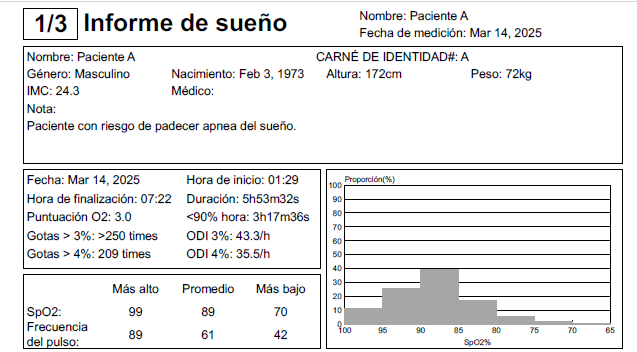
\includegraphics[width=0.85\textwidth]{img/informeSueño.png}
    \caption{Resumen del informe de sueño del dispositivo O2Ring para un caso compatible con apnea moderada.}
    \label{fig:informeO2Ring}
\end{figure}


\section{Técnicas y herramientas}

Esta sección recoge las herramientas de programación, bibliotecas y plataformas utilizadas para desarrollar el sistema predictivo y su despliegue en una aplicación web funcional. Se incluyen también referencias a los entornos de desarrollo y sistemas de documentación empleados, justificando su elección en función de su adecuación técnica al contexto sanitario y computacional del sistema.

\subsection{Python}

Python es un lenguaje de programación interpretado, de alto nivel y de propósito general, ampliamente utilizado en ciencia de datos, inteligencia artificial y desarrollo web. Su sintaxis sencilla, estructura modular y ecosistema de bibliotecas especializadas lo convierten en una herramienta ideal para proyectos de análisis de datos en entornos clínicos.

En este proyecto, Python se ha utilizado como lenguaje base para implementar todo el flujo de trabajo: desde la carga y el preprocesamiento de los datos hasta el entrenamiento, validación, calibración e interpretación del modelo. Además, permitió la construcción de la aplicación web interactiva mediante el framework Streamlit, así como la generación automática de informes en PDF. Su versatilidad ha sido clave para integrar, de forma eficiente y coherente, las diferentes fases del sistema desarrollado \cite{python2024}. 


\subsection{Jupyter Notebook}

Jupyter Notebook es una aplicación web de código abierto que permite crear y compartir documentos interactivos que combinan código ejecutable, visualizaciones, fórmulas matemáticas y texto explicativo. Está especialmente diseñada para entornos de ciencia de datos, aprendizaje automático y análisis computacional, y se ha convertido en una herramienta estándar en investigación y docencia.

Aunque admite múltiples lenguajes de programación mediante el uso de kernels, su integración con Python es la más extendida. Una de sus principales ventajas es la posibilidad de estructurar el trabajo en celdas independientes, lo que permite ejecutar fragmentos de código por separado, visualizar resultados en tiempo real e ir documentando el proceso paso a paso. Esto facilita la validación iterativa, el análisis exploratorio de datos y la depuración eficiente del flujo de trabajo.

En el presente proyecto, Jupyter Notebook se utilizó durante las fases de exploración, preprocesamiento, entrenamiento del modelo y visualización de resultados. Su entorno interactivo ha permitido documentar el desarrollo de forma ordenada, facilitando tanto el análisis como la futura reproducibilidad del sistema construido. \cite{jupyter2024}


\subsection{Anaconda Navigator}

Anaconda es una distribución de código abierto ampliamente utilizada en entornos científicos y de ciencia de datos, ya que facilita la instalación y gestión de entornos virtuales, paquetes y dependencias en Python. Incorpora más de 250 bibliotecas populares preinstaladas, incluyendo \texttt{Pandas}, \texttt{NumPy}, \texttt{scikit-learn}, \texttt{matplotlib} y muchas otras, lo que agiliza el proceso de configuración del entorno de desarrollo.

Dentro de esta distribución, \textbf{Anaconda Navigator} actúa como una interfaz gráfica que permite gestionar entornos, lanzar herramientas como Jupyter Notebook, Spyder o VSCode, e instalar nuevas bibliotecas sin necesidad de comandos en terminal. Esta facilidad de uso lo convierte en una herramienta ideal para proyectos multidisciplinares, especialmente en contextos como la ingeniería de la salud, donde se busca acelerar el desarrollo y garantizar la reproducibilidad.

En este proyecto se utilizó Anaconda para gestionar el entorno de trabajo, instalar todas las dependencias necesarias y organizar los paquetes empleados en las fases de análisis, modelado e implementación de la aplicación. \cite{anaconda2024}


\subsection{Pandas y Numpy}
Pandas es una biblioteca de Python especializada en la manipulación y análisis de datos en estructuras tabulares. Permite trabajar con objetos de tipo \texttt{DataFrame}, que representan conjuntos en formato fila-columna similar a una hoja de cálculo o una tabla SQL. Esta herramienta facilita tareas como la lectura de archivos, limpieza de datos, conversión de tipos...

En este proyecto, Pandas se utilizó en todas las fases del tratamiento de datos: desde la carga inicial del conjunto en formato CSV hasta la transformación de variables, el análisis exploratorio y la preparación del dataset para su posterior entrada al modelo.

Por otro lado, \textbf{Numpy} es una librería orientada al cálculo científico. Proporciona una estructura eficiente para trabajar con \textbf{arrays multidimensionales}, además de incluir funciones matemáticas y estadísticas vectorizadas de alto rendimiento. Fue utilizada de forma complementaria para operaciones aritméticas sobre columnas numéricas y para asegurar un procesamiento rápido y preciso de datos a gran escala.

\subsection{SHAP}

\textbf{SHAP} (SHapley Additive exPlanations) es una librería de Python que permite interpretar modelos de aprendizaje automático complejos mediante la teoría de los valores de Shapley, desarrollada en el marco de los juegos cooperativos. Esta técnica asigna a cada variable una contribución cuantitativa al resultado de una predicción, permitiendo explicar de forma transparente cómo se ha llegado a una determinada clasificación.

En el presente proyecto, SHAP se utilizó para analizar el modelo final (Random Forest) desde dos enfoques complementarios: global e individual. A nivel global, se generaron gráficos resumen (\textit{summary plots}) que muestran la importancia media de cada variable en todas las predicciones. A nivel individual, se aplicaron \textit{force plots} que descomponen la predicción para un usuario específico, visualizando cómo cada variable influye positiva o negativamente en el resultado.

La incorporación de SHAP ha sido clave para garantizar la interpretabilidad del sistema, un aspecto esencial en contextos relacionados con la salud, donde es necesario justificar cada decisión automatizada de forma comprensible y clínicamente relevante.

\subsection{Matplotlib y Seaborn}

\textbf{Matplotlib} y \textbf{Seaborn} son bibliotecas de visualización de datos en Python que permiten generar gráficos personalizados con gran control sobre el estilo y la presentación. Matplotlib proporciona una base versátil para construir figuras a bajo nivel, mientras que Seaborn ofrece una capa de abstracción más sencilla para crear visualizaciones estadísticas complejas con menos código.

Estas herramientas se emplearon en las fases de análisis exploratorio de datos (EDA), visualización de correlaciones, detección de valores atípicos y representación gráfica de resultados. Entre las visualizaciones generadas se encuentran histogramas, gráficos de densidad (KDE), diagramas de caja y violín, mapas de calor (\textit{heatmaps}), matrices de confusión y gráficos de importancia de variables.


\subsection{Streamlit}

Streamlit es un framework de código abierto diseñado para crear aplicaciones web interactivas directamente desde scripts de Python, sin necesidad de conocimientos en desarrollo frontend. Permite transformar scripts de análisis y modelos predictivos en interfaces web funcionales con muy poco código adicional, lo que lo convierte en una herramienta ideal para proyectos de ciencia de datos aplicada y prototipos clínicos.

Entre sus principales ventajas se encuentran la facilidad de uso, su compatibilidad con bibliotecas populares como \texttt{Pandas}, \texttt{scikit-learn} y \texttt{matplotlib}, y la capacidad de actualizar resultados en tiempo real conforme el usuario introduce nuevos datos.

En este proyecto, Streamlit se empleó para construir una aplicación web interactiva que permite al usuario introducir datos clínicos y de estilo de vida, generar una predicción automática sobre el trastorno del sueño más probable, y visualizar una explicación personalizada del resultado mediante gráficos de SHAP. La herramienta fue desplegada en la nube mediante \textit{Streamlit Community Cloud}, garantizando su accesibilidad desde cualquier navegador sin necesidad de instalación. \cite{streamlit}


\subsection{FPDF}
\textbf{FPDF} es una librería de código abierto utilizada para la creación de archivos PDF desde scripts de Python. Gracias a su flexibilidad de diseño y sintaxis intuitiva permite generar informes personalizados y documentos portables.

En el presente proyecto, FPDF fue empleada dentro de la aplicación web interactiva para construir informes automáticos. Estos documentos resumen los datos introducidos por el usuario, la predicción generada por el modelo y una representación visual explicativa basada en SHAP. El objetivo fue proporcionar al usuario un documento descargable que pueda guardar, imprimir o compartir, facilitando así la continuidad del seguimiento clínico o la consulta posterior.

\subsection{Visual Studio}

\textbf{Visual Studio Code} (VS Code) es un entorno de desarrollo integrado (IDE) de código abierto desarrollado por Microsoft. Se caracteriza por su ligereza, extensibilidad y compatibilidad multiplataforma. Permite programar en múltiples lenguajes, entre ellos Python, C++, JavaScript y C\#, y ofrece funcionalidades como resaltado de sintaxis, autocompletado inteligente, depuración paso a paso, control de versiones mediante Git y terminal integrada.

Durante el desarrollo de este proyecto, VS Code fue utilizado como entorno principal para organizar los scripts en Python, estructurar la lógica de predicción, integrar la aplicación en Streamlit y realizar pruebas funcionales del sistema. Su compatibilidad con entornos virtuales, su integración con GitHub y su interfaz modular facilitaron un flujo de trabajo limpio, ordenado y eficiente.

\subsection{GitHub}
\textbf{GitHub} es una plataforma para el control de versiones y la gestión de proyectos basada en el sistema Git. Permite almacenar, organizar y versionar el código fuente de forma colaborativa, además de ofrecer herramientas para documentación, seguimiento de cambios y despliegue de aplicaciones.

En este proyecto, GitHub fue utilizado como repositorio central para el código del modelo, los scripts de preprocesamiento y la implementación de la aplicación web. Gracias a este sistema se garantizó la trazabilidad del desarrollo, la seguridad frente a pérdidas accidentales de información y la posibilidad de reproducir el trabajo completo en futuros entornos.

\subsection{LaTex (Overleaf)}
\textbf{LaTeX} es un sistema de composición tipográfica de alta calidad, ampliamente utilizado en la redacción de documentos técnicos y científicos. Permite estructurar contenidos con precisión, insertar fórmulas matemáticas complejas, generar índices automáticos y gestionar bibliografía de forma eficiente.

Para la redacción de esta memoria se ha utilizado la plataforma \textbf{Overleaf}, un editor LaTeX en línea que permite la escritura colaborativa, el seguimiento de versiones y la integración de paquetes personalizados. Esta herramienta ha sido clave para presentar los contenidos del trabajo con claridad, rigor formal y formato profesional, incluyendo gráficos, referencias cruzadas y citación bibliográfica automatizada.

\subsection{O$_2$ Insight Pro}

\textbf{O$_2$ Insight Pro} es el software oficial del dispositivo portátil \textit{O2Ring} (Viatom), utilizado para visualizar, analizar y exportar datos fisiológicos registrados durante el sueño. Este programa permite extraer variables como la saturación de oxígeno (SpO$_2$), la frecuencia cardíaca, el número de eventos de desaturación y el índice ODI.

Aunque no formó parte del sistema implementado, se utilizó durante la fase de validación externa para obtener registros reales de pacientes y comprobar el comportamiento del modelo ante casos clínicos simulados. Los datos exportados desde O$_2$ Insight Pro se integraron manualmente en el conjunto de entrada de la aplicación, permitiendo una comparación cualitativa entre predicción y perfil fisiológico real.
\capitulo{5}{Resultados}
\label{cap:resultados}

\section{Evaluación comparativa de modelos}
\label{sec:evaluacion_modelos}

\subsection{Evaluación detallada y métricas clave}

Como primer paso para seleccionar el modelo más adecuado, se entrenaron cinco algoritmos de clasificación multiclase utilizando los datos originales del conjunto de entrenamiento, sin aplicar técnicas de balanceo ni ajuste de hiperparámetros. El objetivo de esta fase inicial fue obtener una visión general del rendimiento de cada modelo en condiciones estándar y valorar su comportamiento en un contexto clínico realista.

Los modelos evaluados fueron:

\begin{itemize}
    \item Regresión Logística
    \item Árbol de Decisión
    \item Máquina de Vectores Soporte (SVM)
    \item Random Forest
    \item Perceptrón Multicapa (MLP)
\end{itemize}

Cada modelo fue entrenado con validación cruzada estratificada (k=5), y se calcularon métricas fundamentales como \textbf{accuracy}, \textbf{F1-score macro}, \textbf{recall} por clase y \textbf{precisión} en la clase \texttt{Sleep Apnea}, de especial relevancia clínica.

En la Tabla~\ref{tab:comparativa-inicial} se muestran los resultados obtenidos por cada modelo en esta primera evaluación en condiciones estándar:

\begin{table}[H]
\centering
\small 
\begin{tabular}{lccccc}
\toprule
\textbf{Modelo} & \textbf{Accuracy} & \textbf{F1 Macro} & \textbf{Recall Ins.} & \textbf{Recall Apn.} & \textbf{Prec. Apn.} \\
\midrule
Random Forest       & 0.95 & 0.92 & 0.87 & 0.94 & 0.88 \\
MLP                 & 0.92 & 0.88 & 0.87 & 0.81 & 0.81 \\
Logistic Regression & 0.93 & 0.91 & 0.87 & 0.94 & 0.83 \\
Decision Tree       & 0.92 & 0.89 & 0.93 & 0.81 & 0.87 \\
SVM                 & 0.92 & 0.91 & 0.87 & 0.88 & 0.88 \\
\bottomrule
\end{tabular}
\caption{Rendimiento comparativo de los modelos en condiciones iniciales (sin ajuste ni balanceo).}
\label{tab:comparativa-inicial}
\end{table}

Para profundizar en la evaluación individual de los modelos, en las Figuras~\ref{fig:confusion_logreg} y~\ref{fig:metricas_logreg} se presentan los resultados iniciales del modelo \textit{Logistic Regression}, incluyendo su matriz de confusión y un resumen de métricas cuantitativas obtenidas con \texttt{classification\_report}. Este modelo se ha seleccionado como ejemplo representativo por su equilibrio entre rendimiento global e interpretabilidad, y se utiliza aquí para ilustrar el proceso de evaluación antes de aplicar técnicas de mejora.


\begin{figure}[H]
    \centering
    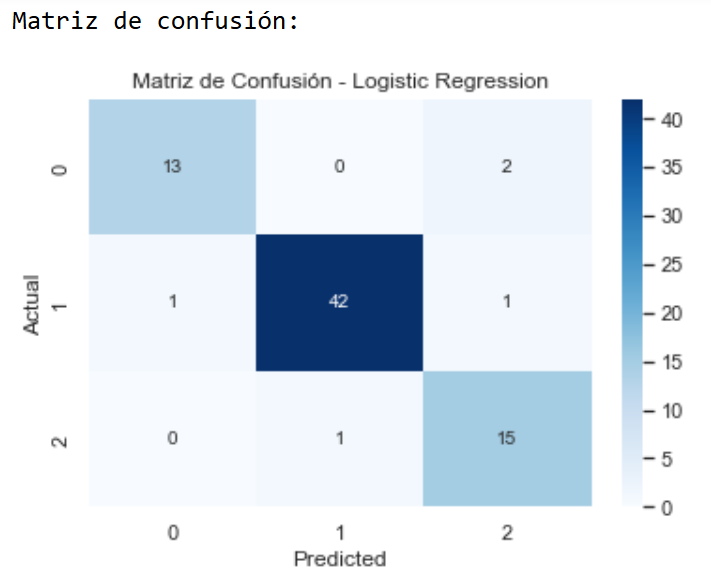
\includegraphics[width=0.6\linewidth]{img/matriz_confusion_logreg.png}
    \caption{Matriz de confusión del modelo \textit{Logistic Regression} sobre el conjunto de test.}
    \label{fig:confusion_logreg}
\end{figure}

\begin{figure}[H]
    \centering
    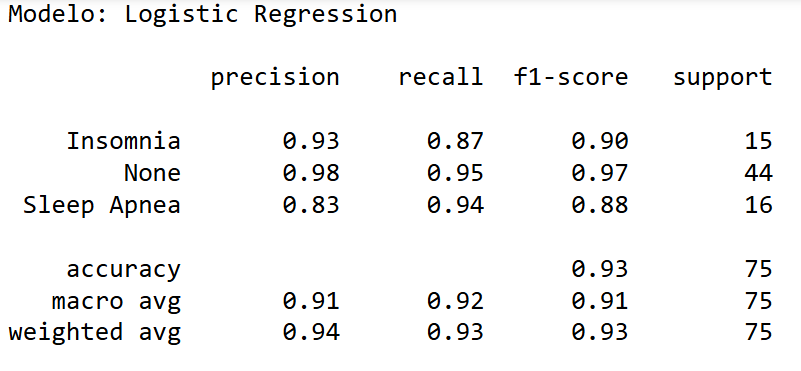
\includegraphics[width=0.65\linewidth]{img/metricas_logreg.png}
    \caption{Resumen de métricas del modelo \textit{Logistic Regression} generadas con \texttt{classification\_report} de \texttt{scikit-learn}.}
    \label{fig:metricas_logreg}
\end{figure}

Tal como se aprecia en la Tabla~\ref{tab:comparativa-inicial}, los modelos \textit{Random Forest} y \textit{Logistic Regression} destacan por sus elevados valores de \textit{accuracy} (0.95 y 0.93 respectivamente) y \textit{F1-score macro} (0.92 y 0.91), manteniendo además un rendimiento sólido en las clases patológicas. En particular, ambos modelos presentan un \textit{recall} en la clase \texttt{Sleep Apnea} de 0.94, lo que resulta clínicamente relevante. En cambio, el modelo \textit{MLP}, muestra menor sensibilidad en dicha clase (0.81), lo cual podría limitar su utilidad como herramienta de cribado inicial. 

Estos resultados iniciales constituyeron la base para aplicar estrategias de mejora, comenzando por el balanceo de clases mediante la técnica SMOTE, cuyo impacto se analiza a continuación.

\subsection{Impacto del balanceo con SMOTE}

Con el fin de analizar el impacto del desbalance de clases, se comparó el rendimiento de cinco modelos entrenados sobre los datos originales y sobre un conjunto equilibrado mediante la técnica \textbf{SMOTE} (Synthetic Minority Over-sampling Technique). Esta técnica genera nuevas muestras sintéticas para las clases minoritarias a partir de sus vecinos más cercanos, con el objetivo de mitigar los sesgos introducidos por el desequilibrio de clases.

Se entrenaron cinco modelos de clasificación bajo ambas condiciones: Regresión Logística, Árbol de Decisión, Máquina de Vectores Soporte (SVM), Random Forest y Perceptrón Multicapa (MLP).


Para cada modelo se calcularon métricas como \textit{accuracy}, \textit{F1-score macro} y \textit{recall} en la clase \texttt{Sleep Apnea}, considerada de mayor relevancia clínica. En la Tabla~\ref{tab:smote_comparacion} se muestra un resumen de estas métricas para facilitar la comparación inicial entre modelos con y sin SMOTE:


\begin{table}[H]
\centering
\resizebox{\textwidth}{!}{%
\begin{tabular}{|l|c|c|c|c|c|c|}
\hline
\rowcolor[HTML]{DAE8FC}
\textbf{Modelo} & \textbf{Accuracy (SMOTE)} & \textbf{Accuracy (No SMOTE)} & \textbf{F1 Macro (SMOTE)} & \textbf{F1 Macro (No SMOTE)} & \textbf{Recall Apnea (SMOTE)} & \textbf{Recall Apnea (No SMOTE)} \\
\hline
Logistic Regression & 0.93 & 0.93 & 0.92 & 0.91 & 1.00 & 0.94 \\
Decision Tree       & 0.93 & 0.91 & 0.91 & 0.87 & 0.94 & 0.81 \\
SVM                 & 0.92 & 0.92 & 0.90 & 0.91 & 1.00 & 0.88 \\
MLP                 & 0.92 & 0.92 & 0.89 & 0.88 & 0.81 & 0.81 \\
Random Forest       & 0.93 & 0.95 & 0.90 & 0.92 & 0.81 & 0.94 \\
\hline
\end{tabular}
}
\caption{Comparación resumida de rendimiento con y sin SMOTE.}
\label{tab:smote_comparacion}
\end{table}

A modo ilustrativo, se muestran a continuación las métricas detalladas y matrices de confusión del modelo \textit{Logistic Regression}, en ambos escenarios:

\begin{figure}[H]
    \centering
    \begin{minipage}{0.48\linewidth}
        \centering
        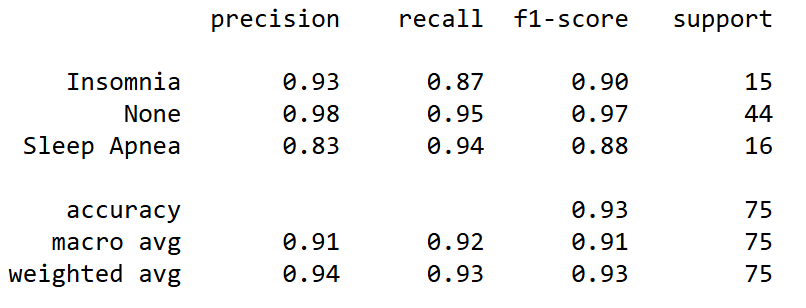
\includegraphics[width=\linewidth]{img/tablaLRsinSmote.png}
        \caption{Métricas del modelo \textit{Logistic Regression} sin SMOTE.}
        \label{fig:tabla_lr_sin_smote}
    \end{minipage}
    \hfill
    \begin{minipage}{0.48\linewidth}
        \centering
        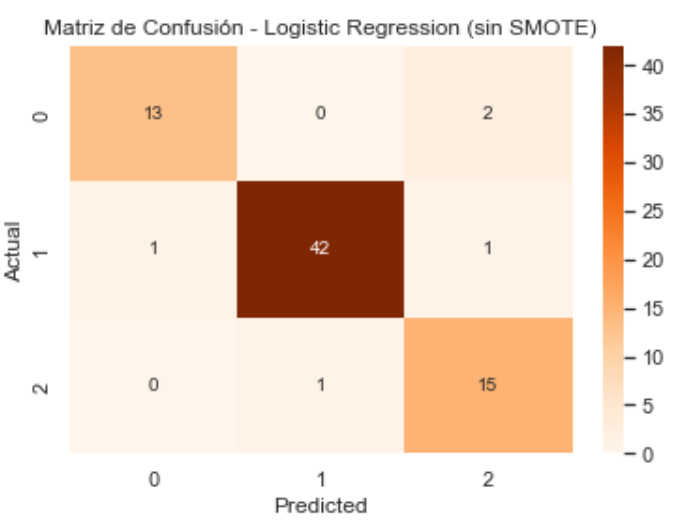
\includegraphics[width=\linewidth]{img/matrizLRsinSmote.png}
        \caption{Matriz de confusión del modelo \textit{Logistic Regression} sin SMOTE.}
        \label{fig:matriz_lr_sin_smote}
    \end{minipage}
\end{figure}

\begin{figure}[H]
    \centering
    \begin{minipage}{0.48\linewidth}
        \centering
        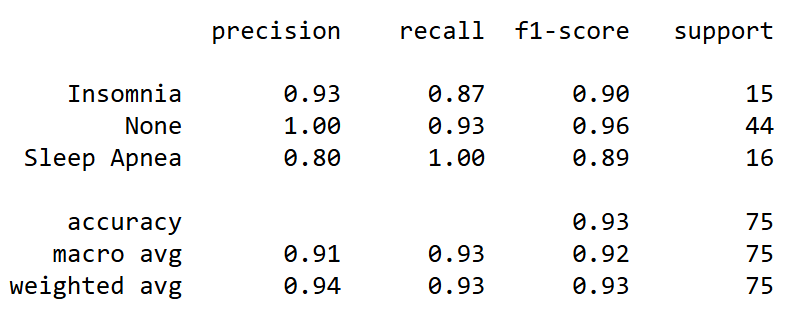
\includegraphics[width=\linewidth]{img/tablaLRsmote.png}
        \caption{Métricas del modelo \textit{Logistic Regression} con SMOTE.}
        \label{fig:tabla_lr_smote}
    \end{minipage}
    \hfill
    \begin{minipage}{0.48\linewidth}
        \centering
        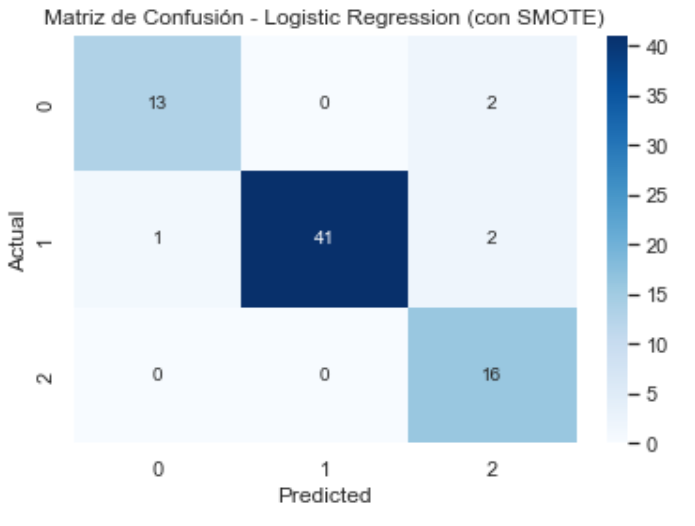
\includegraphics[width=\linewidth]{img/matrizLRsmote.png}
        \caption{Matriz de confusión del modelo \textit{Logistic Regression} con SMOTE.}
        \label{fig:matriz_lr_smote}
    \end{minipage}
\end{figure}

Además, la Figura~\ref{fig:comparativa_smote} muestra un análisis completo con todas las métricas evaluadas para los cinco modelos:

\begin{figure}[H]
    \centering
    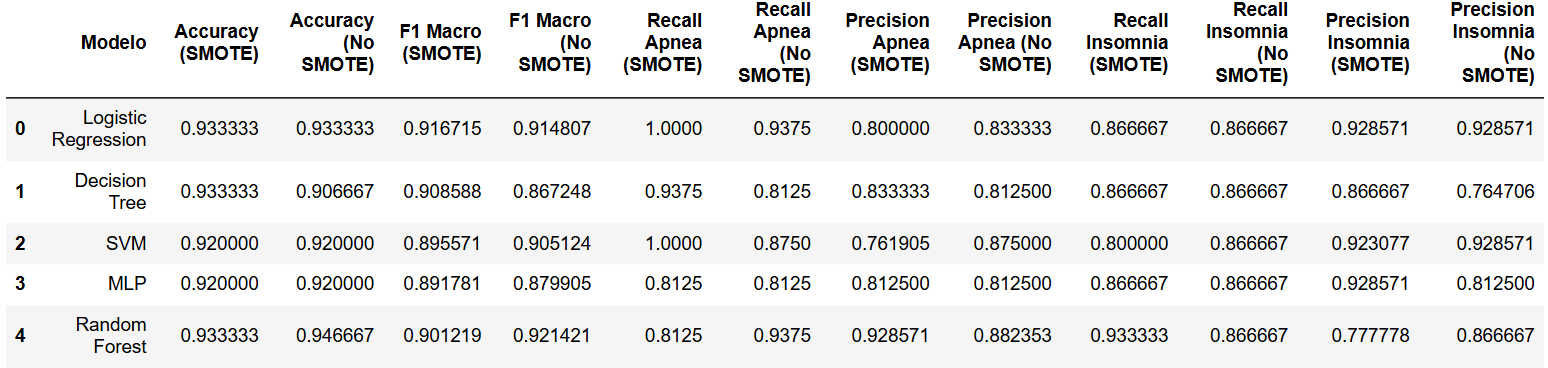
\includegraphics[width=1\linewidth]{img/comparativa_smote.png}
    \caption{Comparación de métricas clave con y sin SMOTE en los cinco modelos.}
    \label{fig:comparativa_smote}
\end{figure}


Los resultados mostraron que SMOTE mejora sistemáticamente el \textit{recall} de la clase \textit{Sleep Apnea} en la mayoría de modelos, lo cual es clínicamente positivo al tratarse de una clase minoritaria. Sin embargo, este aumento suele ir acompañado de una ligera caída en la \textit{precisión}, lo que sugiere un mayor número de falsos positivos.

En el caso de \textit{Logistic Regression}, por ejemplo, el \textit{recall} de \texttt{Sleep Apnea} pasó de 0.94 a 1.00 con SMOTE, pero su precisión cayó del 0.83 al 0.80. En modelos como \textit{Decision Tree}, el \textit{recall} también aumentó significativamente (0.81 → 0.94), aunque sin mejoras globales contundentes. Por el contrario, en el modelo \textit{MLP}, SMOTE no aportó mejoras relevantes, manteniendo el mismo \textit{recall} (0.81) y reduciendo ligeramente la precisión.

En el caso de \textit{Random Forest}, aplicar SMOTE redujo inesperadamente el \textit{recall} de \textit{Sleep Apnea} (de 0.94 a 0.81), indicando una posible pérdida de sensibilidad tras el sobremuestreo.


Dado que el impacto de SMOTE fue inconsistente entre modelos, y considerando el riesgo de sobreajuste en ciertos casos, se optó por no incluir esta técnica en la versión final del sistema. En su lugar, se utilizó la opción \texttt{class\_weight='balanced'} junto con calibración probabilística posterior, lo que permitió mantener un buen rendimiento sin comprometer la estabilidad del modelo.


\subsection{Ajuste de hiperparámetros y calibración}

Con el objetivo de mejorar el rendimiento predictivo de cada modelo, se realizó un proceso de búsqueda de hiperparámetros empleando las funciones \texttt{GridSearchCV} o \texttt{RandomizedSearchCV}, en función del tamaño del espacio de búsqueda y del coste computacional. Esta optimización se llevó a cabo sobre el conjunto de entrenamiento utilizando validación cruzada estratificada con \texttt{cv=5}.

Según el tipo de modelo, se definió como métrica objetivo el \texttt{accuracy} o, en modelos más sensibles al desbalance, el \texttt{F1-score macro}, priorizando así un compromiso entre precisión y sensibilidad global. En la Tabla~\ref{tab:hiperparametros_optimos} se resumen los mejores hiperparámetros encontrados para cada algoritmo:

\begin{table}[H]
\centering
\resizebox{\textwidth}{!}{%
\begin{tabular}{|l|l|}
\hline
\rowcolor[HTML]{DAE8FC}
\textbf{Modelo} & \textbf{Mejores hiperparámetros encontrados} \\
\hline
\textbf{Random Forest} &
\begin{tabular}[c]{@{}l@{}}n\_estimators = 100, max\_depth = None, min\_samples\_leaf = 2, \\ min\_samples\_split = 2, bootstrap = False\end{tabular} \\
\hline
\textbf{MLPClassifier} &
\begin{tabular}[c]{@{}l@{}}hidden\_layer\_sizes = (50,), activation = tanh, solver = adam, \\ alpha = 0.01, learning\_rate = constant\end{tabular} \\
\hline
\textbf{Decision Tree} &
\begin{tabular}[c]{@{}l@{}}criterion = gini, max\_depth = None, min\_samples\_split = 10, \\ min\_samples\_leaf = 4\end{tabular} \\
\hline
\textbf{Logistic Regression} &
\begin{tabular}[c]{@{}l@{}}penalty = l2, solver = liblinear, C = 10\end{tabular} \\
\hline
\textbf{SVM (SVC)} &
\begin{tabular}[c]{@{}l@{}}kernel = poly, C = 0.1, gamma = scale\end{tabular} \\
\hline
\end{tabular}%
}
\caption{Mejores hiperparámetros obtenidos tras la búsqueda para cada modelo.}
\label{tab:hiperparametros_optimos}
\end{table}


Tras seleccionar los hiperparámetros óptimos, se procedió a calibrar las probabilidades de salida para los modelos con mejor rendimiento: \textbf{Random Forest} y \textbf{MLP}. La calibración se realizó mediante la técnica \texttt{CalibratedClassifierCV}, empleando el método \texttt{sigmoid} y validación cruzada interna.

Este ajuste permitió mejorar la fiabilidad de las probabilidades predichas, aspecto especialmente relevante en contextos clínicos donde no solo importa la clase asignada, sino también el grado de confianza en la decisión del sistema.

La comparativa final de resultados se analiza posteriormente en esta sección.


\subsection{Evaluación gráfica con curvas ROC-AUC y Precision-Recall}

Para complementar las métricas cuantitativas obtenidas tras el ajuste de hiperparámetros, se generaron representaciones gráficas que permiten analizar con mayor profundidad el comportamiento de los modelos. En concreto, se visualizaron tres elementos clave: la matriz de confusión, la curva ROC-AUC y la curva Precision-Recall. Estas herramientas permiten estudiar el rendimiento a distintos umbrales de decisión, algo fundamental en escenarios clínicos donde minimizar los falsos negativos es prioritario, pero sin generar un exceso de falsos positivos.

Mientras que la curva ROC-AUC evalúa la capacidad global del modelo para discriminar entre clases, la curva Precision-Recall es especialmente útil en contextos con clases desbalanceadas, ya que refleja directamente el compromiso entre sensibilidad (recall) y la proporción de verdaderos positivos entre las predicciones positivas (precisión).

\subsubsection{Ejemplo representativo: Logistic Regression}

La Figura~\ref{fig:curvas_lr} muestra los resultados visuales del modelo \textit{Logistic Regression}, incluyendo su matriz de confusión, curva ROC-AUC y curva Precision-Recall. Este modelo fue seleccionado como ejemplo representativo debido a su rendimiento equilibrado y su interpretabilidad, y sirve para ilustrar el enfoque seguido en todos los casos.


\begin{figure}[H]
    \centering
    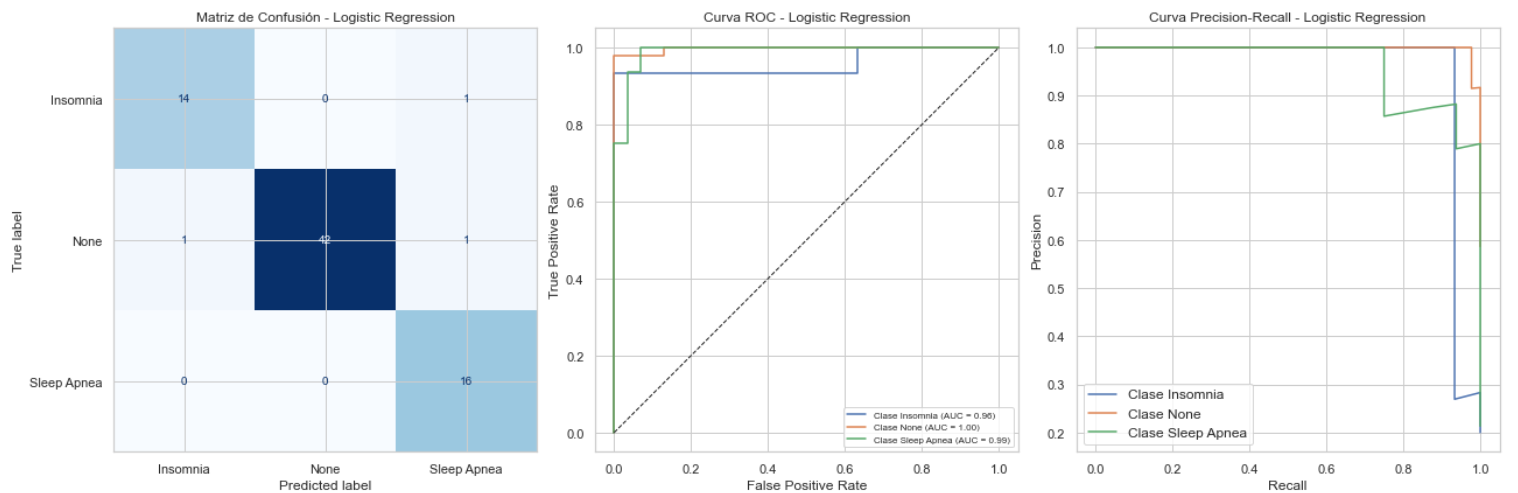
\includegraphics[width=\textwidth]{img/curvas_LR.png}
    \caption{Evaluación visual del modelo \textit{Logistic Regression}: matriz de confusión, curva ROC-AUC y Precision-Recall.}
    \label{fig:curvas_lr}
\end{figure}

\subsubsection{Comparación de curvas ROC-AUC por clase}

A continuación se muestran las curvas ROC-AUC de los cinco modelos, diferenciadas por clase. Esta representación permite observar con mayor detalle el rendimiento discriminativo para cada tipo de trastorno del sueño. 

\begin{figure}[H]
    \centering
    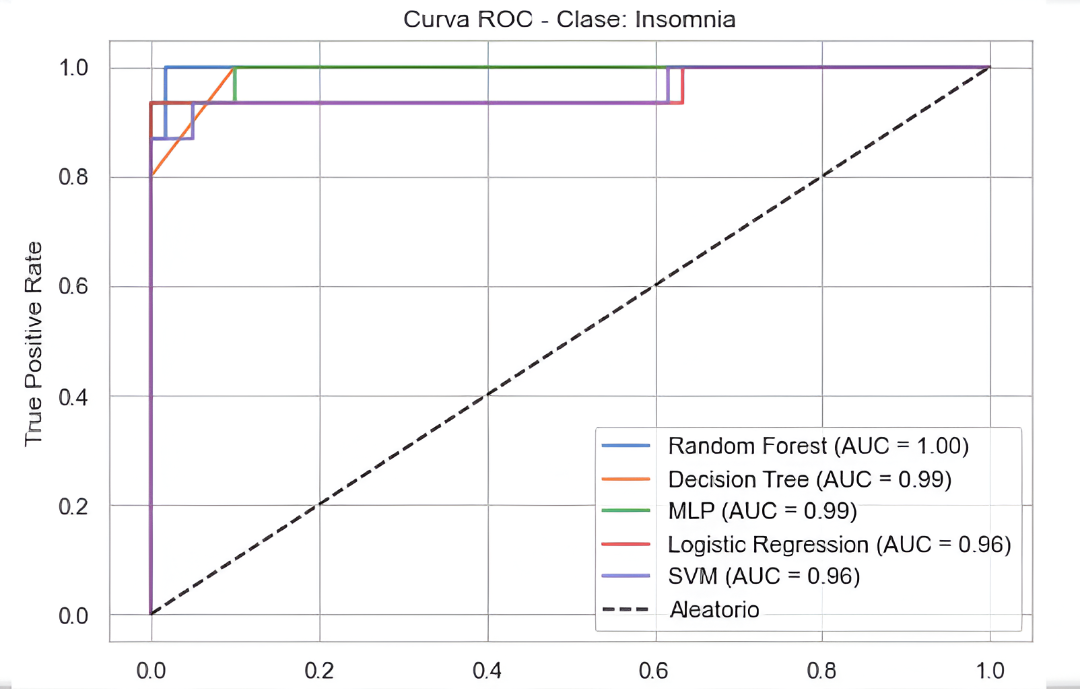
\includegraphics[width=0.9\textwidth]{img/roc_insomnia.png}
    \caption{Curva ROC-AUC para la clase \texttt{Insomnia}.}
    \label{fig:roc_insomnia}
\end{figure}

\begin{figure}[H]
    \centering
    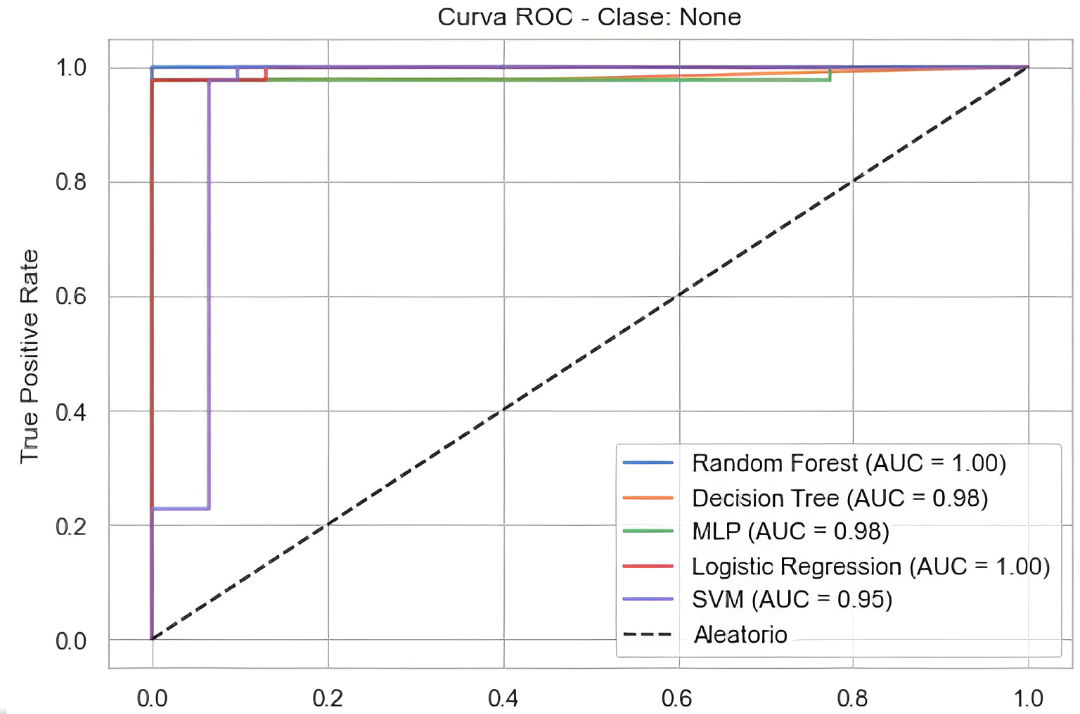
\includegraphics[width=0.9\textwidth]{img/roc_none.png}
    \caption{Curva ROC-AUC para la clase \texttt{None}.}
    \label{fig:roc_none}
\end{figure}

\begin{figure}[H]
    \centering
    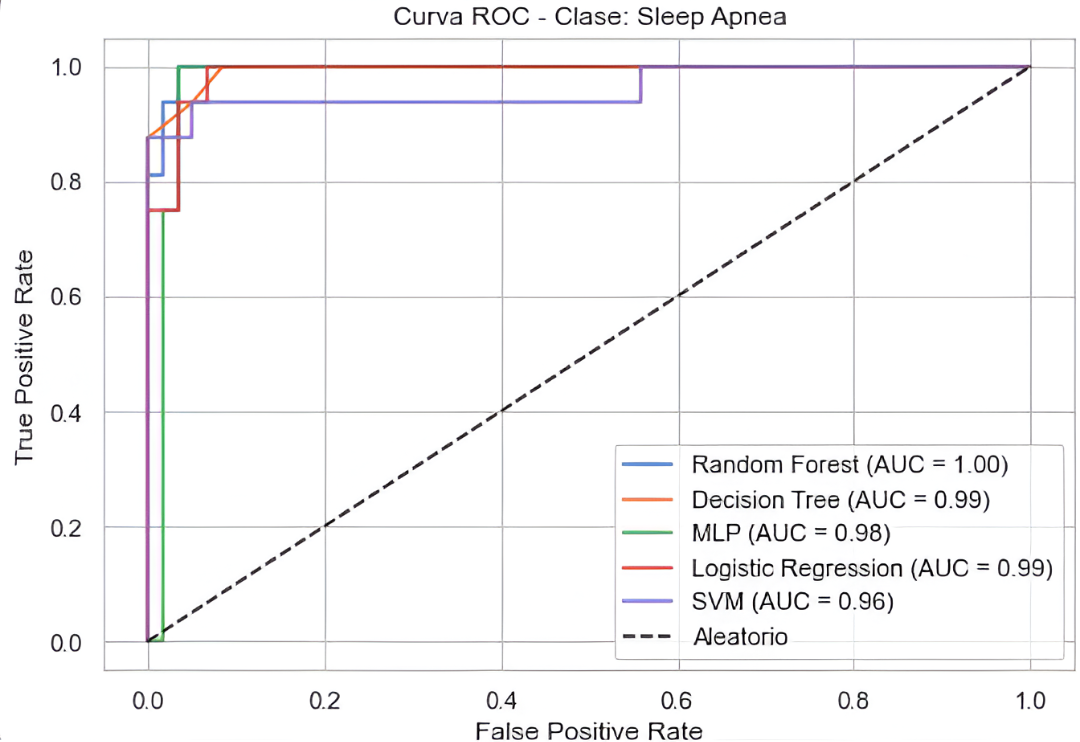
\includegraphics[width=0.8\textwidth]{img/roc_apnea.png}
    \caption{Curva ROC-AUC para la clase \texttt{Sleep Apnea}.}
    \label{fig:roc_apnea}
\end{figure}

Se observa que los modelos \textit{Random Forest} y \textit{MLP} mantienen una capacidad discriminativa sobresaliente en todas las clases, con áreas bajo la curva (AUC) superiores al 0.98. Este comportamiento se mantiene especialmente estable en la clase \texttt{Sleep Apnea}, lo que resulta crítico desde un punto de vista clínico, ya que permite minimizar los falsos negativos en una condición potencialmente grave.

El modelo \textit{Logistic Regression} también muestra un desempeño competitivo, alcanzando un AUC de 1.00 en la clase \texttt{None} y de 0.96 en \texttt{Insomnia} y \texttt{Sleep Apnea}, lo cual refleja su equilibrio entre precisión y sensibilidad.

Por su parte, el modelo \textit{SVM} presenta una ligera caída en el AUC en todas las clases (entre 0.95 y 0.96), aunque aún dentro de un margen aceptable. \textit{Decision Tree} tiene un rendimiento intermedio, con AUC de 0.98--0.99, pero con una curva más irregular.

Estas diferencias sugieren que, aunque todos los modelos son razonablemente fiables, \textit{Random Forest} y \textit{MLP} ofrecen mayor robustez en situaciones clínicas reales donde la correcta discriminación entre clases es fundamental.

\vspace{1em}

\subsubsection{Comparación de curvas Precision-Recall por clase}

A continuación se presentan las curvas Precision-Recall, especialmente relevantes en contextos con clases desbalanceadas. Estas permiten evaluar la capacidad del modelo para mantener una alta precisión a medida que se incrementa la sensibilidad.


\begin{figure}[H]
    \centering
    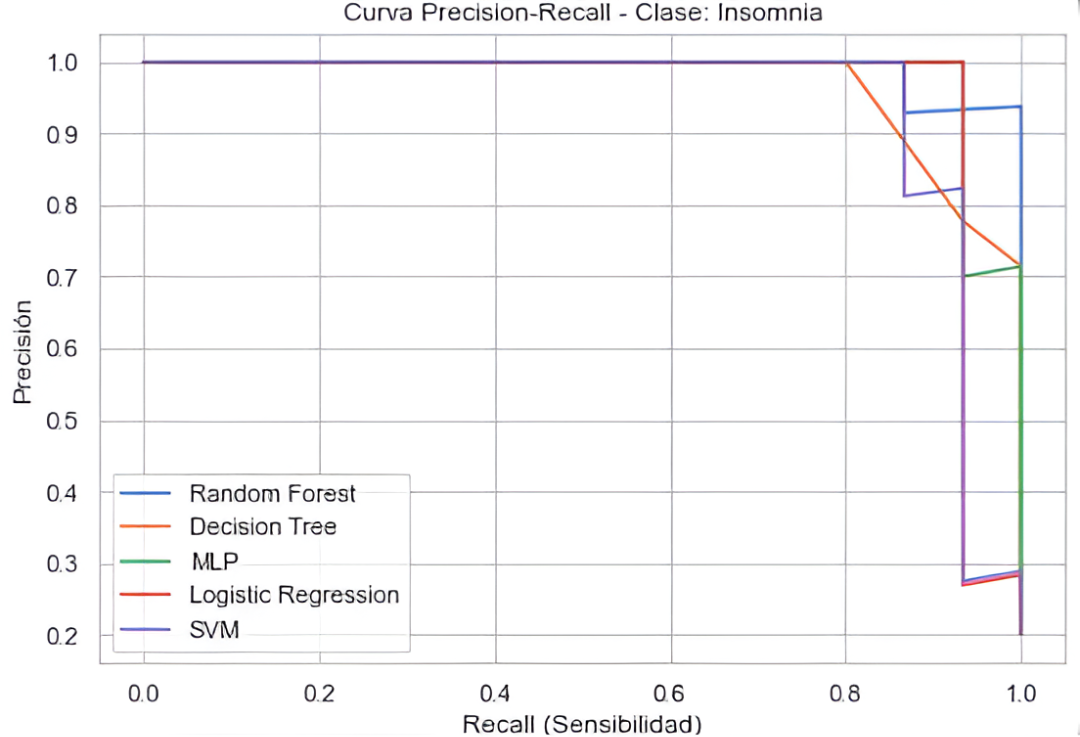
\includegraphics[width=0.8\textwidth]{img/pr_insomnia.png}
    \caption{Curva Precision-Recall para la clase \texttt{Insomnia}.}
    \label{fig:pr_insomnia}
\end{figure}

\begin{figure}[H]
    \centering
    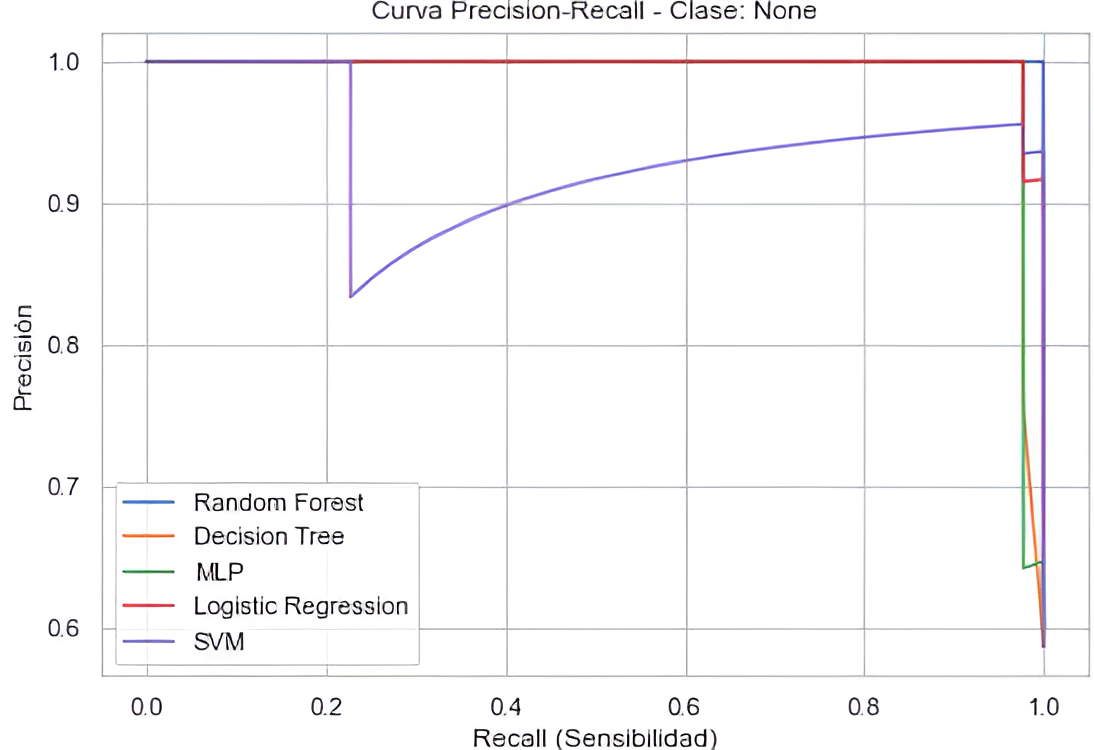
\includegraphics[width=0.8\textwidth]{img/pr_none.png}
    \caption{Curva Precision-Recall para la clase \texttt{None}.}
    \label{fig:pr_none}
\end{figure}

\begin{figure}[H]
    \centering
    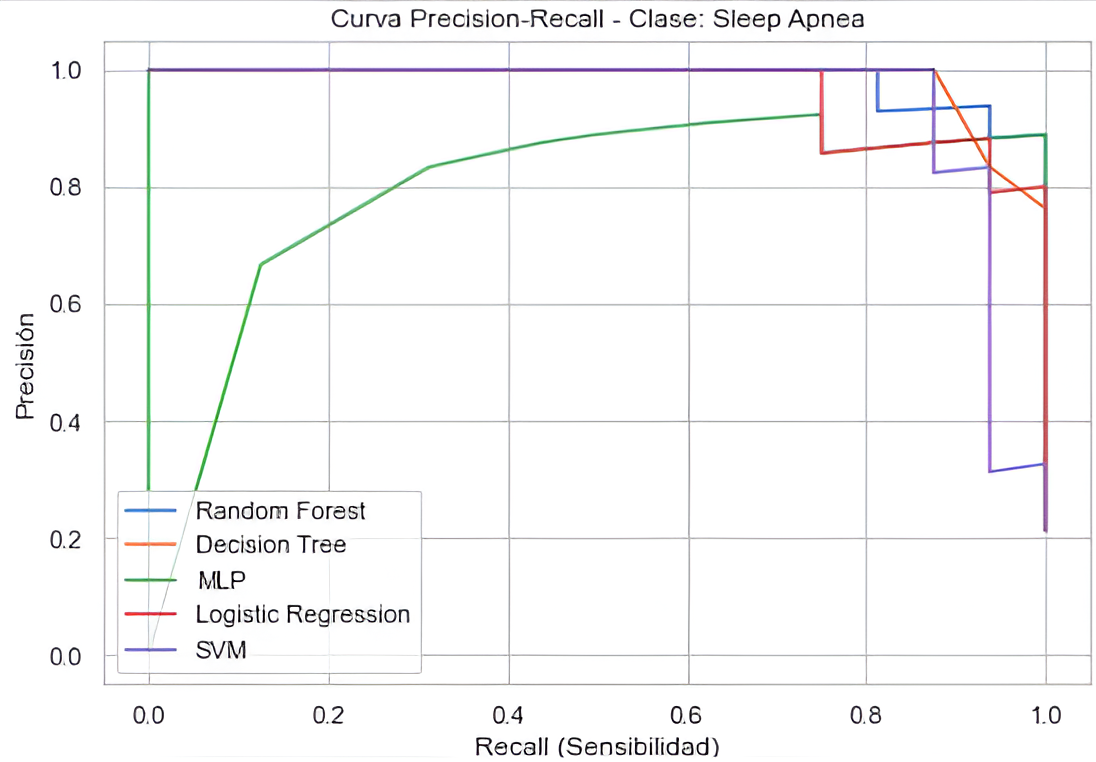
\includegraphics[width=0.8\textwidth]{img/pr_apnea.png}
    \caption{Curva Precision-Recall para la clase \texttt{Sleep Apnea}.}
    \label{fig:pr_apnea}
\end{figure}

En cuanto a las curvas Precision-Recall, se reafirma el buen comportamiento de \textit{Random Forest} y \textit{MLP}, especialmente en las clases minoritarias. En \texttt{Sleep Apnea}, \textit{Random Forest} mantiene una alta precisión incluso con niveles elevados de recall, lo que indica que logra identificar a la mayoría de los casos positivos sin generar un exceso de falsos positivos.

\textit{MLP}, por su parte, destaca en la clase \texttt{Insomnia}, mostrando una curva más estable y cercana al óptimo. Esto refuerza su idoneidad en entornos clínicos donde la sensibilidad debe ser prioritaria.

En contraste, modelos como \textit{SVM} y \textit{Decision Tree} presentan curvas más irregulares y una caída más abrupta de la precisión a medida que aumenta el recall, lo cual podría comprometer su fiabilidad en un sistema de cribado automatizado.

Estas curvas confirman que no solo es importante qué clase se predice, sino también con qué confianza lo hace el modelo, un aspecto clave cuando se trata de emitir alertas médicas.


\subsubsection{Resumen conjunto de desempeño por clase}

El análisis gráfico detallado permite identificar patrones diferenciales en el comportamiento de los modelos por clase. En la clase \texttt{Insomnia}, los modelos Random Forest y MLP ofrecen curvas ROC-AUC y Precision-Recall elevadas y estables, lo que sugiere una buena capacidad para detectar esta condición con alta sensibilidad sin comprometer la precisión. En cambio, modelos como SVM o Decision Tree muestran ligeros descensos en la precisión, indicando mayor tendencia a generar falsos positivos.

\begin{table}[H]
\centering
\small
\begin{tabular}{lccc|ccc}
\toprule
\multirow{2}{*}{\textbf{Modelo}} & \multicolumn{3}{c|}{\textbf{AUC-ROC}} & \multicolumn{3}{c}{\textbf{AUC-PR}} \\
& \textbf{Insomnia} & \textbf{None} & \textbf{Apnea} & \textbf{Insomnia} & \textbf{None} & \textbf{Apnea} \\
\midrule
Random Forest       & 1.00 & 1.00 & 1.00 & 0.94 & 0.99 & 0.96 \\
MLP                 & 0.99 & 0.98 & 0.98 & 0.87 & 0.98 & 0.93 \\
Logistic Regression & 0.96 & 1.00 & 0.99 & 0.93 & 1.00 & 0.91 \\
Decision Tree       & 0.99 & 0.98 & 0.99 & 0.89 & 0.99 & 0.88 \\
SVM                 & 0.96 & 0.95 & 0.96 & 0.91 & 0.94 & 0.87 \\
\bottomrule
\end{tabular}
\caption{Comparativa de AUC-ROC y AUC-PR por clase en los cinco modelos evaluados.}
\label{tab:auc-por-clase}
\end{table}

La Tabla~\ref{tab:auc-por-clase} refuerza este análisis al mostrar los valores medios de las métricas AUC-ROC y AUC-PR para cada clase. Se confirma que Random Forest y MLP alcanzan los mejores resultados en la clase \texttt{Insomnia}, destacando en ambas métricas sobre el resto.

Para la clase \texttt{None}, todos los modelos alcanzan valores muy altos de AUC y precisión, lo que es esperable dado que se trata de la clase mayoritaria y, por tanto, más representada durante el entrenamiento. Esto refuerza la necesidad de priorizar el análisis específico en las clases clínicas más relevantes.

En el caso de \texttt{Sleep Apnea}, la curva Precision-Recall de MLP destaca por mantener un recall próximo al 1.0, aunque con menor precisión en ciertos rangos de umbral. Random Forest, en cambio, presenta un mayor equilibrio entre ambas métricas, siendo capaz de identificar correctamente la mayoría de los casos sin aumentar el número de falsos positivos de forma excesiva. Esto lo convierte en un candidato sólido para su implementación en la herramienta final, donde el balance clínico entre sensibilidad y especificidad es crucial.

En conjunto, la descomposición por clase de estas curvas ofrece una perspectiva rica y más precisa que las métricas globales, reforzando la validez del análisis multiclase en un contexto sanitario.


\subsection{Comparación final y selección del modelo óptimo}

Tras analizar las métricas cuantitativas y los resultados gráficos, se seleccionaron dos modelos como los más prometedores durante la fase experimental: \textbf{Random Forest} y \textbf{MLP}. Ambos presentaron un rendimiento sobresaliente en las métricas evaluadas —\textit{accuracy}, \textit{F1-score macro}, \textit{recall} y \textit{precisión}—, así como una excelente capacidad discriminativa entre clases.

La elección se basó tanto en los valores obtenidos como en las curvas ROC-AUC y Precision-Recall, que confirmaron un comportamiento consistente y fiable. Ambos modelos compartían las siguientes características clave:


\begin{itemize}
    \item Área bajo la curva (AUC) superior a 0.95 en todas las clases.
    \item Buen equilibrio entre precisión y sensibilidad, especialmente en \texttt{Sleep Apnea}.
    \item Estabilidad en distintas particiones del conjunto de validación.
\end{itemize}

\textbf{Random Forest} destacó por su mayor interpretabilidad y precisión en la clase \texttt{Sleep Apnea}, lo que facilita su trazabilidad en entornos clínicos. Por su parte, \textbf{MLP} alcanzó un \textit{recall} perfecto en esa misma clase, lo que resulta ventajoso en contextos donde se prioriza la sensibilidad diagnóstica para minimizar falsos negativos.


Ambos modelos fueron evaluados como candidatos finales, pero finalmente se seleccionó Random Forest para su integración definitiva en la aplicación por su capacidad explicativa. Este modelo fue calibrado mediante \texttt{CalibratedClassifierCV} y guardado en el archivo:

\begin{itemize}
  \item \texttt{random\_forest\_model.joblib}
\end{itemize}

La validación práctica y externa de este modelo, incluyendo su evaluación con datos del dispositivo O2Ring, se detalla en la siguiente sección.


\subsection{Evaluación comparativa con y sin la variable \texttt{Occupation}}

Con el objetivo de evaluar el impacto real de la variable \texttt{Occupation} en la capacidad predictiva del modelo, se construyó una versión alternativa del sistema eliminando dicha característica del conjunto de entrenamiento. Esta modificación tenía como objetivo analizar si la ocupación laboral estaba introduciendo un sesgo en las predicciones, y si el modelo era capaz de mantener un rendimiento clínico aceptable sin dicha información. Cabe señalar que algunas ocupaciones estaban sobrerrepresentadas en ciertas clases del conjunto de entrenamiento, lo que podría inducir al modelo a establecer falsas asociaciones.

Para garantizar un análisis controlado, se mantuvieron constantes todas las demás variables, de forma que cualquier cambio en la predicción pudiera atribuirse exclusivamente a la presencia o ausencia de la variable \texttt{Occupation}. La validación se realizó sobre tres perfiles clínicos reales representativos: un paciente con apnea del sueño (A), un sujeto sano (B) y un paciente con insomnio leve (C). Las predicciones se compararon entre ambas versiones del modelo, manteniendo los parámetros fisiológicos constantes (edad, sexo, IMC) y ajustando únicamente variables como pasos diarios, duración del sueño o nivel de estrés para reforzar la coherencia clínica.

\begin{table}[H]
\centering
\begin{tabular}{|c|c|c|c|c|}
\hline
\textbf{Paciente} & \textbf{Diagnóst esperado} & \textbf{Con Occupation} & \textbf{Sin Occupation} \\
\hline
A (Apnea)   & Apnea del sueño     & Sleep Apnea (70.0\%) & Insomnia (59.0\%) \\
B (Sano)    & Ninguno             & Sleep Apnea (59.0\%) & None (98.0\%) \\
C (Insomnio) & Insomnio subjetivo & Sleep Apnea (58.0\%) & Insomnia (67.0\%) \\
\hline
\end{tabular}
\caption{Comparativa de predicciones entre ambas versiones del modelo usando los perfiles clínicos reales.}
\end{table}


Los resultados revelan un patrón claro: la versión \textbf{con la variable \texttt{Occupation}} tiende a \textbf{sobrediagnosticar apnea del sueño} en todos los casos, incluso cuando no hay evidencia clínica suficiente, como ocurre con los pacientes B y C. Esta tendencia sugiere un sobreajuste del modelo o un sesgo inducido por la ocupación laboral.

Por el contrario, la versión \textbf{sin \texttt{Occupation}} mostró un comportamiento más prudente y clínicamente coherente. Fue capaz de clasificar correctamente al paciente sano y de aproximarse mejor a la predicción esperada en el caso de insomnio, aunque aún presenta margen de mejora en sensibilidad. Este comportamiento indica que, si bien la variable \texttt{Occupation} aporta poder predictivo, también introduce un riesgo clínico si no se maneja cuidadosamente.

En consecuencia, se optó por mantener el modelo con \texttt{Occupation} calibrado como núcleo del sistema desplegado, dada su estabilidad, calibración previa y compatibilidad con las herramientas de interpretabilidad. No obstante, se incorporaron advertencias explícitas en la interfaz sobre el carácter orientativo del sistema y la posible influencia de variables contextuales. Esta evaluación pone de manifiesto la importancia de revisar críticamente el uso de variables categóricas con fuerte carga contextual y de diseñar mecanismos de mitigación de sesgos en futuros desarrollos clínicos.


\section{Validación externa con datos reales del dispositivo O2Ring}

Con el objetivo de evaluar la capacidad del modelo para generalizar fuera del conjunto de entrenamiento, se realizó una validación externa utilizando datos fisiológicos recogidos con el pulsioxímetro comercial O2Ring. Esta prueba permite estimar el rendimiento del sistema en condiciones clínicas reales.

Se seleccionaron tres pacientes reales con perfiles representativos de las tres clases objetivo del problema: apnea del sueño, individuo sano e insomnio leve. A continuación se resume su análisis individual.


\subsection{Paciente A – Apnea del sueño}

\begin{itemize}
    \item Edad: 57 años, IMC: 31.8 (obesidad)
    \item Duración del sueño: 5h 53min
    \item Saturación media: 89\%, mínima: 70\%
    \item Tiempo con SpO\textsubscript{2} < 90\%: 3h 17min
    \item ODI 3\%: 43.3/h
    \item FC media: 61 bpm
\end{itemize}

\textbf{Diagnóstico clínico esperado:} Apnea moderada-grave.
\textbf{Predicción del modelo:} Sleep Apnea (70.4\%).  
\textbf{¿Acertó?} Sí.

\subsection{Paciente B – Perfil sano}

\begin{itemize}
    \item Edad: 32 años, IMC: 20.6 (peso normal)
    \item Duración del sueño: 8h 28min
    \item Saturación media: 96\%, mínima: 92\%
    \item ODI 3\%: 0.1/h, SpO\textsubscript{2} < 90\%: 0s
    \item FC media: 51 bpm
\end{itemize}

\textbf{Diagnóstico clínico esperado:} Sin trastornos.  
\textbf{Predicción del modelo:} Sleep Apnea (56.0\%).  
\textbf{¿Acertó?} No (falso positivo).

\subsection{Paciente C – Perfil compatible con insomnio}

\begin{itemize}
    \item Edad: 55 años, IMC: 25.4 (límite sobrepeso)
    \item Duración del sueño: 7h, calidad: 4/10
    \item Estrés alto, 1 día de deporte semanal, 5000 pasos diarios
    \item Presión arterial: 120/75, FC: 48 bpm
\end{itemize}

\textbf{Diagnóstico clínico esperado:} Insomnio leve subjetivo.  
\textbf{Predicción del modelo:} Sleep Apnea (72.7\%).  
\textbf{¿Acertó?} No (falso positivo).


\subsection{Resumen de resultados}

\begin{table}[H]
\centering
\begin{tabular}{|c|c|c|c|c|}
\hline
\textbf{Paciente} & \textbf{Diagnóstico esperado} & \textbf{Predicción} & \textbf{¿Acertó?} \\
\hline
A & Apnea del sueño & Sleep Apnea (70.4\%) & Sí \\
B & Ninguno         & Sleep Apnea (60.0\%) & No \\
C & Insomnio        & Sleep Apnea (72.7\%) & No \\
\hline
\end{tabular}
\caption{Validación externa con datos reales recogidos mediante O2Ring.}
\end{table}


Los resultados de esta validación externa revelan limitaciones importantes del sistema desplegado. Aunque en el caso A se acertó el diagnóstico con alta probabilidad, los casos B y C fueron clasificados erróneamente como apnea del sueño, a pesar de que sus métricas fisiológicas no justificaban dicho diagnóstico.

Estos errores confirman que el modelo, entrenado exclusivamente con variables demográficas y de estilo de vida, carece de sensibilidad suficiente para distinguir correctamente entre insomnio, sujetos sanos y apnea real. La ausencia de variables biométricas clave como SpO$_2$ nocturna, ODI o eventos respiratorios limita la capacidad clínica del sistema para ofrecer diagnósticos fiables.

Este análisis pone de manifiesto la necesidad de incorporar señales fisiológicas reales en futuras versiones del modelo, así como de realizar entrenamientos con conjuntos de datos validados clínicamente. Solo así será posible desarrollar sistemas de ayuda al diagnóstico que sean realmente útiles y seguros en entornos reales.

\section{Discusión}

Este trabajo ha demostrado la viabilidad de desarrollar un sistema predictivo funcional para la detección automática de trastornos del sueño, empleando exclusivamente datos clínicos y de estilo de vida. La implementación completa del pipeline —desde la preparación de datos hasta la validación externa y la integración en una aplicación web— permite reflexionar sobre la utilidad real de este tipo de herramientas, sus limitaciones actuales y sus implicaciones futuras.


\subsection{Importancia de las métricas en el contexto clínico}

En un entorno sanitario, no todas las métricas de evaluación tienen el mismo peso. Aunque el \textit{accuracy} proporciona una visión general del rendimiento del modelo, puede resultar engañosa en problemas con clases desbalanceadas o consecuencias clínicas asimétricas.

En este estudio, se priorizó el \textbf{recall} en la clase \texttt{Sleep Apnea}, dado que no detectar un caso real puede tener consecuencias graves para el paciente. Por ello, este indicador se consideró crítico en todas las fases de evaluación y selección del modelo, especialmente al comparar candidatos como \textit{Random Forest} y \textit{MLP}.


\subsection{Errores comunes y clases más conflictivas}

Durante las validaciones, tanto internas como externas, se observó que la clase \texttt{Sleep Apnea} concentraba la mayoría de los errores, especialmente en forma de falsos positivos. El sistema tendía a sobrediagnosticar esta clase en perfiles donde no existía evidencia clínica suficiente, como ocurrió con los pacientes B y C durante la validación externa.

En contraste, la clase \texttt{Insomnia} fue identificada con mayor estabilidad en varios modelos, lo que sugiere que sus rasgos subjetivos (calidad del sueño, duración baja, estrés elevado) estaban mejor representados en los datos y eran más fáciles de distinguir estadísticamente.



\subsection{Limitaciones del sistema y del conjunto de datos}

Las principales limitaciones que condicionan el rendimiento clínico del sistema son:

\begin{itemize}
    \item \textbf{Tamaño reducido del dataset}: solo 374 registros, lo que limita la generalización del modelo a poblaciones reales más diversas.
    \item \textbf{Datos autodeclarados}: variables como la calidad del sueño, el nivel de estrés o la duración del sueño están basadas en percepciones subjetivas del paciente, introduciendo sesgos de respuesta.
    \item \textbf{Desequilibrio de clases}: la clase \texttt{None} representa más del 50\% del total, lo que afecta a la estabilidad del aprendizaje y puede favorecer predicciones triviales.
    \item \textbf{Ausencia de datos fisiológicos reales}: el modelo no conoce variables clave como SpO$_2$, ODI, eventos respiratorios o movimiento nocturno, lo que limita su valor clínico.
\end{itemize}

Aunque se evaluaron técnicas de balanceo como SMOTE, sus efectos no fueron consistentes, y en algunos casos derivaron en sobreajuste. Se optó por enfoques más conservadores como el ajuste de pesos de clase y la calibración probabilística.

\subsection{Impacto de la variable \texttt{Occupation}}

Uno de los hallazgos más relevantes del estudio fue el impacto de la variable \texttt{Occupation} en las predicciones. El modelo entrenado con esta variable mostró un sesgo claro hacia la clase \texttt{Sleep Apnea}, clasificando erróneamente perfiles sanos o compatibles con insomnio como casos de apnea, incluso tras modificar otras variables.

La comparación con una versión del modelo sin \texttt{Occupation} reveló un comportamiento más prudente y alineado con el diagnóstico esperado en varios casos. Sin embargo, este modelo alternativo no fue integrado en la aplicación final, ya que no estaba calibrado ni preparado para su despliegue. Aun así, la existencia de este sesgo justifica plenamente la incorporación de advertencias explícitas en la app y refuerza la necesidad de revisar críticamente el uso de variables socioeconómicas en contextos clínicos.


\subsection{Relación con la literatura}

Los resultados obtenidos son coherentes con estudios previos que emplean modelos de machine learning para el cribado de trastornos del sueño a partir de datos tabulados. El trabajo de \textit{Alnour et al. (2024)}\footnote{\cite{alnour2024kaggle}}, base del dataset utilizado, ya demostraba que modelos como \textit{Random Forest} o \textit{SVM} ofrecían buen rendimiento en tareas de clasificación, aunque sin explorar su integración práctica.

Este proyecto ha ido un paso más allá al incluir explicabilidad mediante SHAP, validación con pacientes reales monitorizados con O2Ring, y la implementación completa de una aplicación web interactiva y descargable.


\subsection{Implicaciones y proyección}

A pesar de sus limitaciones, el sistema propuesto presenta potencial como herramienta de cribado preliminar o de concienciación en contextos sin acceso a polisomnografía ni actigrafía. Su facilidad de uso, la interpretabilidad integrada y la generación automática de informes podrían facilitar su adopción en entornos comunitarios o de atención primaria.

Sin embargo, la validación con pacientes reales ha puesto de manifiesto que la fiabilidad clínica del modelo es limitada si no se integran variables fisiológicas reales. En este sentido, se propone como línea futura la recogida de datos multimodales —incluyendo señales del sueño, pulsioximetría y movimiento— que permitan entrenar modelos más precisos y clínicamente útiles.

Los siguientes capítulos recogen las conclusiones generales del trabajo y propuestas concretas para su mejora.
 \capitulo{6}{Conclusiones}

A lo largo del desarrollo de este Trabajo Fin de Grado se ha conseguido construir un sistema predictivo capaz de estimar la probabilidad de que un paciente presente insomnio, apnea del sueño o no presente trastornos, a partir de variables clínicas, demográficas y de estilo de vida. El proyecto ha integrado herramientas de ciencia de datos con ingeniería de software, ofreciendo una solución funcional, explicable e interactiva, orientada tanto a profesionales como a usuarios no expertos.

Desde el punto de vista técnico, se han cumplido los principales objetivos planteados. Se ha realizado un análisis exploratorio riguroso del conjunto de datos, un preprocesamiento exhaustivo de sus variables y el desarrollo comparativo de cinco modelos de clasificación multiclase. Finalmente, se seleccionó un modelo \textbf{Random Forest calibrado y balanceado}, que ofreció un rendimiento robusto y explicable mediante técnicas SHAP. Este modelo fue integrado con éxito en una aplicación web desarrollada con Streamlit, accesible desde dispositivos móviles y capaz de generar informes clínicos en PDF de forma automatizada.

El sistema desarrollado tiene potencial como herramienta de \textbf{cribado inicial o sensibilización}, facilitando una evaluación rápida del riesgo de trastornos del sueño en poblaciones no diagnosticadas. Además, sienta las bases para futuras versiones más avanzadas, con integración de sensores biométricos o seguimiento longitudinal.

\section{Aspectos relevantes}

Durante el desarrollo del proyecto se tomaron decisiones clave que influyeron directamente en la calidad final del sistema. Aunque inicialmente se valoró utilizar datos fisiológicos reales mediante el dispositivo O2Ring, se optó por trabajar con un conjunto de datos clínico estructurado y de libre acceso, lo que permitió focalizar los esfuerzos en el diseño, validación y despliegue del modelo.

Uno de los mayores retos fue lidiar con el desequilibrio entre clases, ya que la clase mayoritaria ("None") concentraba más del 50\% de los registros del dataset. Este desbalance podía inducir al modelo a predecir sistemáticamente la clase más frecuente, penalizando la detección de trastornos como el insomnio o la apnea. En una primera fase se exploró la técnica SMOTE (Synthetic Minority Oversampling Technique), generando ejemplos sintéticos para las clases minoritarias. Aunque esta técnica mejoró el \textit{recall} en algunos modelos, también introdujo ruido y sobreajuste en otros, especialmente en Random Forest, reduciendo su capacidad de generalización.

Ante esta situación, se decidió finalmente descartar SMOTE y optar por una combinación de estrategias más conservadoras y robustas. En primer lugar, se aplicó el parámetro \texttt{class\_weight='balanced'} en los clasificadores que lo permitían, ajustando automáticamente el peso de cada clase en función de su frecuencia. En segundo lugar, se incorporó una calibración de probabilidades mediante \texttt{CalibratedClassifierCV}, lo que permitió mejorar la fiabilidad de las predicciones sin alterar el modelo base. Esta aproximación mantuvo un buen equilibrio entre precisión y sensibilidad en todas las clases, evitando los efectos adversos observados con el sobremuestreo artificial.

El camino seguido pone de manifiesto la importancia de evaluar críticamente cada técnica y no asumir que soluciones comunes (como SMOTE) funcionarán en todos los casos. Esta toma de decisiones iterativa y fundamentada fue clave para obtener un sistema final equilibrado, explicable y robusto frente a datos clínicamente relevantes.


Aunque en la fase de entrenamiento algunos modelos mostraban métricas prometedoras, los resultados finales sobre los datos de test revelaron un rendimiento más modesto de lo esperado, especialmente en ciertas clases clínicas. Este hecho pone de manifiesto la importancia de contar con datos de mayor calidad y diversidad para asegurar una generalización adecuada del modelo. Variables como el estrés, el sueño o la calidad de vida son altamente subjetivas y difíciles de medir con precisión, lo que afecta directamente a la capacidad predictiva del sistema.


La introducción de técnicas de explicabilidad como SHAP ha sido especialmente valiosa, ya que permite interpretar las decisiones del modelo en términos clínicos comprensibles. Esta característica añade transparencia al sistema y facilita su aceptación tanto por parte de usuarios como de profesionales sanitarios.


Desde el punto de vista del desarrollo software, se han integrado múltiples funcionalidades en la app, incluyendo: formulario dinámico, predicción en tiempo real, explicación visual de los resultados, generación de informes en PDF, y acceso móvil mediante QR. Cada uno de estos componentes ha sido documentado e implementado con atención al detalle, facilitando su posible ampliación o mantenimiento futuro.

Durante la fase inicial del desarrollo de la interfaz se consideró también el uso de \textit{Shiny}, una plataforma popular para construir dashboards en el entorno R. Sin embargo, esta opción fue descartada por la falta de integración directa con el ecosistema Python, sobre el que se había implementado todo el pipeline de datos, el entrenamiento de modelos y la lógica de predicción. En su lugar, se optó por utilizar \textbf{Streamlit}, un framework ligero, interactivo y orientado a ciencia de datos que permitió desarrollar rápidamente una interfaz funcional sin necesidad de conocimientos en desarrollo web tradicional. Esta decisión no solo facilitó el despliegue en la nube y la generación de informes PDF personalizados, sino que también permitió mantener una coherencia tecnológica a lo largo de todo el proyecto.

En conjunto, este proyecto ha permitido aplicar de forma integrada conocimientos de machine learning, ingeniería biomédica y desarrollo web. A nivel formativo, ha consolidado competencias técnicas y metodológicas en un contexto realista y multidisciplinar, orientado a resolver un problema de salud pública con potencial impacto.

En definitiva, el sistema desarrollado no constituye un producto clínico validado, pero representa un \textbf{primer paso sólido} hacia herramientas accesibles, interpretables y escalables en salud digital. La metodología seguida y los resultados obtenidos abren nuevas oportunidades para mejorar el cribado precoz, la educación sanitaria y el diseño de sistemas inteligentes centrados en el usuario.

\capitulo{7}{Líneas de trabajo futuras}

El presente proyecto ha demostrado que es viable aplicar modelos de aprendizaje automático para detectar de forma preliminar posibles trastornos del sueño a partir de datos clínicos y de estilo de vida. A pesar de que los resultados obtenidos no han alcanzado en todos los casos el nivel esperado, se ha logrado sentar una base sólida sobre la que seguir construyendo. 

A continuación, se proponen varias líneas de trabajo que podrían abordarse en el futuro para mejorar y ampliar el proyecto desarrollado:

\section{Incorporación de datos fisiológicos en tiempo real}
Una de las mejoras con mayor potencial incluye la integración en la propia aplicación sensores biométricos, como es el caso del O2Ring o wearables comerciales (Fitbit, MiBand, Apple Watch). A partir de estos dispositivos se obtendría información como la saturación de oxígeno, frecuencia cardíaca o interrupciones en el sueño, permitiendo construir un modelo más complejo gracias a la integración de datos subjetivos y objetivos.

\section{Ampliación y validación del conjunto de datos}
Uno de los principales límites del modelo actual es el tamaño y la naturaleza del conjunto de datos utilizado. Aunque ha servido como punto de partida para desarrollar y validar el sistema, sería conveniente rediseñar la arquitectura utilizando tecnologías de backend más escalables y seguras, capaces de soportar una mayor carga de usuarios y garantizar la estabilidad del servicio.

Una posible línea de trabajo sería recopilar nuevos registros provenientes de diferentes contextos clínicos o poblaciones. Esto permitiría no solo aumentar la cantidad de datos disponibles, sino también evaluar la capacidad del modelo para generalizar sus predicciones a distintos perfiles de pacientes.

Además, se podría plantear la creación de una base de datos que integrase tanto información declarativa como variables fisiológicas obtenidas mediante sensores. Esta ampliación del dataset facilitaría entrenar modelos más precisos, así como realizar validaciones cruzadas más exigentes.

Por último, sería conveniente llevar a cabo un proceso de validación externa, en colaboración con profesionales del ámbito clínico, que permita comprobar el rendimiento del sistema fuera del entorno de desarrollo.

 
\section{Validación en entornos reales}

Una vez desarrollado y testado en un entorno controlado, el siguiente paso natural sería validar el sistema en contextos clínicos reales, como consultas de atención primaria, unidades del sueño o programas de cribado en salud pública. Este tipo de validación permitiría evaluar no solo la precisión del modelo en la práctica, sino también su utilidad y aceptación por parte de los profesionales sanitarios. 

Además, sería posible recoger feedback directo sobre aspectos como la facilidad de uso de la aplicación, el tiempo necesario para introducir los datos o el grado de confianza que genera el sistema en los usuarios. Esta información resultaría de gran valor para orientar futuras mejoras funcionales y de diseño.

En paralelo, sería interesante analizar el impacto del sistema en el flujo de trabajo habitual, observando si realmente contribuye a una detección más temprana o a una reducción de derivaciones innecesarias, dos de los objetivos principales del proyecto.

 

\section{Evolución del modelo predictivo}
El modelo actual se basa en un clasificador de tipo \textit{Random Forest}, por su equilibrio entre rendimiento, interpretabilidad y bajo coste computacional. No obstante, en fases futuras podría explorarse el uso de modelos más complejos y adaptativos que permitan capturar mejor las relaciones no lineales entre variables.

Entre las alternativas más prometedoras se encuentran las redes neuronales profundas, especialmente aquellas adaptadas a datos tabulares, o los modelos ensamblados con técnicas avanzadas de \textit{boosting}. Asimismo, podría incorporarse algún mecanismo de aprendizaje continuo que permita actualizar el modelo con nuevos datos sin necesidad de reentrenarlo por completo.

En todos los casos, sería esencial mantener la transparencia y la interpretabilidad del sistema, para garantizar su uso responsable en entornos clínicos. Por ello, sería recomendable combinar estas técnicas con herramientas de \textit{explainable AI} (XAI) como SHAP o LIME.

 


\section{Desarrollo de una versión escalable de la aplicación}

La versión actual de la aplicación, desarrollada con Streamlit, resulta adecuada para prototipado y validación en fases iniciales. Sin embargo, si se desea avanzar hacia un producto utilizable a mayor escala, sería necesario rediseñar la arquitectura con tecnologías más robustas y escalables. 

Finalmente, para garantizar su integración en entornos sanitarios reales, sería clave adaptar la solución a estándares como HL7 o FHIR y contemplar la posibilidad de exportar los resultados directamente a sistemas de historia clínica electrónica (EHR). 

\section{Aplicaciones en salud pública y educación}
Más allá de su uso individual, la herramienta desarrollada podría tener un impacto positivo en el ámbito de la salud pública. Por ejemplo, podría utilizarse en campañas de cribado poblacional para detectar factores de riesgo relacionados con el sueño en entornos escolares, laborales o comunitarios.

Del mismo modo, puede resultar útil como recurso educativo en programas de promoción de la salud, ayudando a sensibilizar a la población sobre la importancia de un sueño adecuado y los efectos de los hábitos de vida en su calidad. La generación automática de informes personalizados refuerza la comprensión de los resultados, aumentando su impacto educativo y clínico.

Por último, en un contexto de medicina preventiva, esta herramienta podría integrarse en estrategias más amplias de digitalización y autocuidado, contribuyendo a empoderar al usuario y a descongestionar los sistemas sanitarios.


Estas líneas de trabajo futuras no solo ofrecen posibles caminos de mejora técnica, sino que reflejan la evolución natural de un sistema que, con una base sólida, aspira a convertirse en una herramienta útil en la práctica clínica y en la educación sanitaria. La combinación de modelos predictivos, explicabilidad, sensores fisiológicos y despliegue accesible representa una tendencia creciente en salud digital, en la que este proyecto se sitúa como primer paso significativo.



\bibliographystyle{apalike}
\bibliography{bibliografia}

\end{document}
